% Options for packages loaded elsewhere
\PassOptionsToPackage{unicode}{hyperref}
\PassOptionsToPackage{hyphens}{url}
%
\documentclass[
]{book}
\title{EBM \& Statistiek III}
\author{\href{mailto:Robby.DePauw@Ugent.be}{\nolinkurl{Robby.DePauw@Ugent.be}}}
\date{2022-01-02}

\usepackage{amsmath,amssymb}
\usepackage{lmodern}
\usepackage{iftex}
\ifPDFTeX
  \usepackage[T1]{fontenc}
  \usepackage[utf8]{inputenc}
  \usepackage{textcomp} % provide euro and other symbols
\else % if luatex or xetex
  \usepackage{unicode-math}
  \defaultfontfeatures{Scale=MatchLowercase}
  \defaultfontfeatures[\rmfamily]{Ligatures=TeX,Scale=1}
\fi
% Use upquote if available, for straight quotes in verbatim environments
\IfFileExists{upquote.sty}{\usepackage{upquote}}{}
\IfFileExists{microtype.sty}{% use microtype if available
  \usepackage[]{microtype}
  \UseMicrotypeSet[protrusion]{basicmath} % disable protrusion for tt fonts
}{}
\makeatletter
\@ifundefined{KOMAClassName}{% if non-KOMA class
  \IfFileExists{parskip.sty}{%
    \usepackage{parskip}
  }{% else
    \setlength{\parindent}{0pt}
    \setlength{\parskip}{6pt plus 2pt minus 1pt}}
}{% if KOMA class
  \KOMAoptions{parskip=half}}
\makeatother
\usepackage{xcolor}
\IfFileExists{xurl.sty}{\usepackage{xurl}}{} % add URL line breaks if available
\IfFileExists{bookmark.sty}{\usepackage{bookmark}}{\usepackage{hyperref}}
\hypersetup{
  pdftitle={EBM \& Statistiek III},
  pdfauthor={Robby.DePauw@Ugent.be},
  hidelinks,
  pdfcreator={LaTeX via pandoc}}
\urlstyle{same} % disable monospaced font for URLs
\usepackage{color}
\usepackage{fancyvrb}
\newcommand{\VerbBar}{|}
\newcommand{\VERB}{\Verb[commandchars=\\\{\}]}
\DefineVerbatimEnvironment{Highlighting}{Verbatim}{commandchars=\\\{\}}
% Add ',fontsize=\small' for more characters per line
\usepackage{framed}
\definecolor{shadecolor}{RGB}{248,248,248}
\newenvironment{Shaded}{\begin{snugshade}}{\end{snugshade}}
\newcommand{\AlertTok}[1]{\textcolor[rgb]{0.94,0.16,0.16}{#1}}
\newcommand{\AnnotationTok}[1]{\textcolor[rgb]{0.56,0.35,0.01}{\textbf{\textit{#1}}}}
\newcommand{\AttributeTok}[1]{\textcolor[rgb]{0.77,0.63,0.00}{#1}}
\newcommand{\BaseNTok}[1]{\textcolor[rgb]{0.00,0.00,0.81}{#1}}
\newcommand{\BuiltInTok}[1]{#1}
\newcommand{\CharTok}[1]{\textcolor[rgb]{0.31,0.60,0.02}{#1}}
\newcommand{\CommentTok}[1]{\textcolor[rgb]{0.56,0.35,0.01}{\textit{#1}}}
\newcommand{\CommentVarTok}[1]{\textcolor[rgb]{0.56,0.35,0.01}{\textbf{\textit{#1}}}}
\newcommand{\ConstantTok}[1]{\textcolor[rgb]{0.00,0.00,0.00}{#1}}
\newcommand{\ControlFlowTok}[1]{\textcolor[rgb]{0.13,0.29,0.53}{\textbf{#1}}}
\newcommand{\DataTypeTok}[1]{\textcolor[rgb]{0.13,0.29,0.53}{#1}}
\newcommand{\DecValTok}[1]{\textcolor[rgb]{0.00,0.00,0.81}{#1}}
\newcommand{\DocumentationTok}[1]{\textcolor[rgb]{0.56,0.35,0.01}{\textbf{\textit{#1}}}}
\newcommand{\ErrorTok}[1]{\textcolor[rgb]{0.64,0.00,0.00}{\textbf{#1}}}
\newcommand{\ExtensionTok}[1]{#1}
\newcommand{\FloatTok}[1]{\textcolor[rgb]{0.00,0.00,0.81}{#1}}
\newcommand{\FunctionTok}[1]{\textcolor[rgb]{0.00,0.00,0.00}{#1}}
\newcommand{\ImportTok}[1]{#1}
\newcommand{\InformationTok}[1]{\textcolor[rgb]{0.56,0.35,0.01}{\textbf{\textit{#1}}}}
\newcommand{\KeywordTok}[1]{\textcolor[rgb]{0.13,0.29,0.53}{\textbf{#1}}}
\newcommand{\NormalTok}[1]{#1}
\newcommand{\OperatorTok}[1]{\textcolor[rgb]{0.81,0.36,0.00}{\textbf{#1}}}
\newcommand{\OtherTok}[1]{\textcolor[rgb]{0.56,0.35,0.01}{#1}}
\newcommand{\PreprocessorTok}[1]{\textcolor[rgb]{0.56,0.35,0.01}{\textit{#1}}}
\newcommand{\RegionMarkerTok}[1]{#1}
\newcommand{\SpecialCharTok}[1]{\textcolor[rgb]{0.00,0.00,0.00}{#1}}
\newcommand{\SpecialStringTok}[1]{\textcolor[rgb]{0.31,0.60,0.02}{#1}}
\newcommand{\StringTok}[1]{\textcolor[rgb]{0.31,0.60,0.02}{#1}}
\newcommand{\VariableTok}[1]{\textcolor[rgb]{0.00,0.00,0.00}{#1}}
\newcommand{\VerbatimStringTok}[1]{\textcolor[rgb]{0.31,0.60,0.02}{#1}}
\newcommand{\WarningTok}[1]{\textcolor[rgb]{0.56,0.35,0.01}{\textbf{\textit{#1}}}}
\usepackage{longtable,booktabs,array}
\usepackage{calc} % for calculating minipage widths
% Correct order of tables after \paragraph or \subparagraph
\usepackage{etoolbox}
\makeatletter
\patchcmd\longtable{\par}{\if@noskipsec\mbox{}\fi\par}{}{}
\makeatother
% Allow footnotes in longtable head/foot
\IfFileExists{footnotehyper.sty}{\usepackage{footnotehyper}}{\usepackage{footnote}}
\makesavenoteenv{longtable}
\usepackage{graphicx}
\makeatletter
\def\maxwidth{\ifdim\Gin@nat@width>\linewidth\linewidth\else\Gin@nat@width\fi}
\def\maxheight{\ifdim\Gin@nat@height>\textheight\textheight\else\Gin@nat@height\fi}
\makeatother
% Scale images if necessary, so that they will not overflow the page
% margins by default, and it is still possible to overwrite the defaults
% using explicit options in \includegraphics[width, height, ...]{}
\setkeys{Gin}{width=\maxwidth,height=\maxheight,keepaspectratio}
% Set default figure placement to htbp
\makeatletter
\def\fps@figure{htbp}
\makeatother
\setlength{\emergencystretch}{3em} % prevent overfull lines
\providecommand{\tightlist}{%
  \setlength{\itemsep}{0pt}\setlength{\parskip}{0pt}}
\setcounter{secnumdepth}{5}
\mainmatter
\ifLuaTeX
  \usepackage{selnolig}  % disable illegal ligatures
\fi

\usepackage{amsthm}
\newtheorem{theorem}{Theorem}[chapter]
\newtheorem{lemma}{Lemma}[chapter]
\newtheorem{corollary}{Corollary}[chapter]
\newtheorem{proposition}{Proposition}[chapter]
\newtheorem{conjecture}{Conjecture}[chapter]
\theoremstyle{definition}
\newtheorem{definition}{Definition}[chapter]
\theoremstyle{definition}
\newtheorem{example}{Example}[chapter]
\theoremstyle{definition}
\newtheorem{exercise}{Exercise}[chapter]
\theoremstyle{definition}
\newtheorem{hypothesis}{Hypothesis}[chapter]
\theoremstyle{remark}
\newtheorem*{remark}{Remark}
\newtheorem*{solution}{Solution}
\begin{document}
\maketitle

{
\setcounter{tocdepth}{2}
\tableofcontents
}
\hypertarget{over-deze-cursus}{%
\chapter*{Over deze cursus}\label{over-deze-cursus}}


De cursus {EBM \& Statistiek III} bouwt verder op de leerstof uit {EBM \& Statistiek I} en {EBM \& Statistiek II}. De situering, vereiste begincompetanties en eindcompetenties zijn terug te vinden op de vak-specifieke pagina op \href{https://ufora.ugent.be}{Ufora}. Binnen deze cursus bespreken we meer geavanceerde statistische modellen. De belangrijkste van deze modellen zijn:

\begin{itemize}
\tightlist
\item
  Bivariate correlaties
\item
  Lineaire regressie
\item
  Logistische regressie
\item
  Mixed models
\item
  Overlevingsanalyses
\end{itemize}

Binnen deze cursus maken we gebruik van enkele oefeningen in {SPSS}


\includegraphics[width=1.04167in,height=\textheight]{img/spss.png}

Probeer voor de oefeningen versie 26 van {SPSS} te gebruiken indien deze beschikbaar is op Athena. Er kan ook steeds een stand-alone versie van {SPSS} aangevraagd worden via volgende \href{https://helpdesk.ugent.be/athena/}{link}. \textbf{Opgelet}: de website met instructies om {SPSS} te installeren op jouw computer is alleen beschikbaar vanuit het UGent netwerk of via VPN.

\hypertarget{de-lesgevers}{%
\section*{De lesgevers}\label{de-lesgevers}}


De lessen binnen het vak worden georganiseerd door \emph{dr. Robby De Pauw} en \emph{prof. dr. Pascal Coorevits}. Vragen kunnen steeds gepost worden in de discussieruimtes op Ufora.

Voor vragen over het stuk statistiek kunnen jullie steeds mailen naar \href{mailto:Robby.DePauw@Ugent.be}{\nolinkurl{Robby.DePauw@Ugent.be}}, voor vragen over het stuk datamanegement kunnen jullie mailen naar \href{mailto:Pascal.Coorevits@Ugent.be}{\nolinkurl{Pascal.Coorevits@Ugent.be}}.

\hypertarget{uitprintversie-boek}{%
\section*{Uitprintversie boek}\label{uitprintversie-boek}}


Bovenaan de balk van deze website kunnen jullie een pdf-versie van dit boek downloaden.

\begin{Shaded}
\begin{Highlighting}[]
\NormalTok{knitr}\SpecialCharTok{::}\FunctionTok{asis\_output}\NormalTok{(}\StringTok{\textquotesingle{}}\SpecialCharTok{\textbackslash{}\textbackslash{}}\StringTok{mainmatter}\SpecialCharTok{\textbackslash{}n\textbackslash{}n}\StringTok{\textquotesingle{}}\NormalTok{)}
\end{Highlighting}
\end{Shaded}

\mainmatter

\hypertarget{intro}{%
\chapter{Introductie}\label{intro}}

In de huidige cursus {EBM \& Statistiek III} wordt er verder gebouwd op de kennis die opgedaan is tijdens de lessen van {EBM \& Statistiek I} en {EBM \& Statistiek II}. Binnen deze lessen werden concepten zoals \textbf{steekproef}, \textbf{beschrijvende statistiek} en \textbf{inferentiële statistiek}. Alle kennis en vaardigheden die jullie binnen de leerlijn \texttt{EBM\ en\ Statistiek} opbouwen, moet jullie in staat stellen om zelfstandig een onderzoeksproces van het begin tot het einde te begrijpen, te beoordelen op kwaliteit en te vertalen naar de klinische praktijk.

Een onderzoekproces bestaat uit verschillende belangrijke stappen die nodig zijn om tot een duidelijk en rechtlijnige conclusie te komen. Enkele basisbegrippen die noodzakelijk zijn om te begrijpen zijn \emph{hypothese}, \emph{fouten} bij hypothesetesten en statistische \emph{toetsen}. Hieronder bespreken we kort deze belangrijke concepten opnieuw. Voor meer informatie verwijzen we naar de cursussen uit {EBM \& Statistiek I} en {EBM \& Statistiek II}.

\hypertarget{hypothesetoetsen}{%
\section*{Hypothesetoetsen}\label{hypothesetoetsen}}


Een hypothesetoets bestaat uit twee delen, de nulhypothese \(H_0\) en de alternatieve hypothese \(H_1\) of \(H_a\). Het uitgangspunt van een hypothesetoets is vaak \(H_0\), waarbij we veronderstellen dat een effect (uitgedrukt als een verschil, associatie, \ldots) niet bestaat. Na het opstellen van een hypothese en de vertaalslag van deze hypothese naar \(H_a\) en \(H_0\), wordt er data verzameld binnen een steekproef. Op basis van deze verzamelde data proberen we \(H_0\) te verwerpen in het voordeel van \(H_a\). De beslissing om \(H_0\) te verwerpen zal uiteindelijk gebeuren op basis van de \(p\)-waarde. Als cut-off wordt hier vaak 5\% (of 0.05) genomen. We noemen deze cut-off ook wel het significantieniveau of \(\alpha\).

Aangenomen wordt dat geen effect geassocieerd wordt met \(H_0\), wat niet betekent dat er geen alternatieve mogelijkheden zijn. We kunnen bijvoorbeeld ook stellen dat we onder \(H_0\) veronderstellen dat een effect een specifiek getal moet zijn (bijvoorbeeld dat het verschil tussen twee groepen exact 2 moet bedragen).

\hypertarget{fouten-bij-hypothesetoetsen}{%
\section*{Fouten bij hypothesetoetsen}\label{fouten-bij-hypothesetoetsen}}


Op basis van een hypothesetoets die we uitvoeren op basis van verzamelde data uit een steekproef van een bepaalde populatie proberen we een besluit te vormen over de hypothese binnen de populatie. Aangezien een steekproef en metingen gepaard gaan met variabiliteit en onzekerheid, kunnen er fouten optreden. In onderstaande tabel vinden jullie een grafische weergave van deze mogelijke fouten:

\begin{figure}
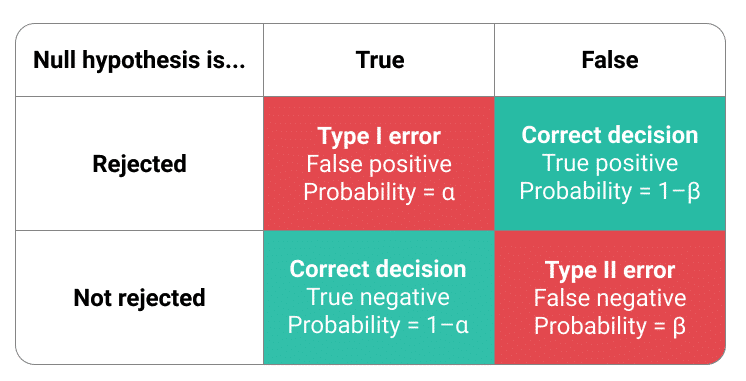
\includegraphics[width=0.9\linewidth]{img/error} \caption{Visuele samenvatting van fouten bij hypothesetoetsen.}\label{fig:error}
\end{figure}

\textbf{Voorbeeld:} Veronderstel dat er binnen de populatie van kinesitherapeuten geen verschil is in het aantal uren die gepresteerd worden tussen mannen en vrouwen. We organiseren binnen deze populatie (\(n = 30\)) en evaluaeren het aantal uren. Uiteindelijk voeren we een statistische toets uit, waaruit we finaal besluiten of er al dan geen verschil is in gepresteerde uren. Hiervoor veronderstellen we volgende hypothesen:

\begin{itemize}
\tightlist
\item
  \(H_0\): Er is geen verschil in gepresteerde uren tussen mannen en vrouwen.
\item
  \(H_1\): Er is een verschil in gepresteerde uren tussen mannen en vrouwen.
\end{itemize}

Indien we binnen de populatie weten dat er \textbf{geen} verschil is (\(H_0\) is dus juist), zijn er twee mogelijke uitkomsten:

\begin{itemize}
\tightlist
\item
  We verwerpen \(H_0\) en besluiten dus dat er wel een verschil is. In dit scenario maken we een fout en binnen de inductieve statistiek wordt deze fout aangeduid als \(\alpha\) (Type I error). Algemeen wordt aanvaard om deze \(\alpha\) op 5\% te zetten.
\item
  We aanvaarden \(H_0\) en besluiten dus dat er wel een verschil is. In dit scenario maken we een correcte beslissing.
\end{itemize}

Indien we binnen de populatie weten dat er \textbf{wel} verschil is (\(H_0\) is dus fout), zijn er twee mogelijke uitkomsten:

\begin{itemize}
\tightlist
\item
  We verwerpen \(H_0\) en besluiten dus dat er wel een verschil is. In dit scenario maken we een correcte beslissing.
\item
  We aanvaarden \(H_0\) en besluiten dus dat er geen verschil is. In dit scenario maken we een fout en binnen de inductieve statistiek wordt deze fout aangeduid als \(\beta\) (Type II error). Over de grootte van \(\beta\) is er minder consensus, maar 80\% wordt vaak algemeen aanvaard.
\end{itemize}

In bovenstaande figuur \ref{fig:error} kan je de \textbf{vier} verschillende scenario's zoals hierboven beschreven herkennen.

\hypertarget{keuze-statistische-toets}{%
\section*{Keuze statistische toets}\label{keuze-statistische-toets}}


In figuur \ref{fig:stattest} vinden jullie een schema met de specifieke keuze van statistische toets op basis van de gestelde voorwaarden.

\begin{figure}
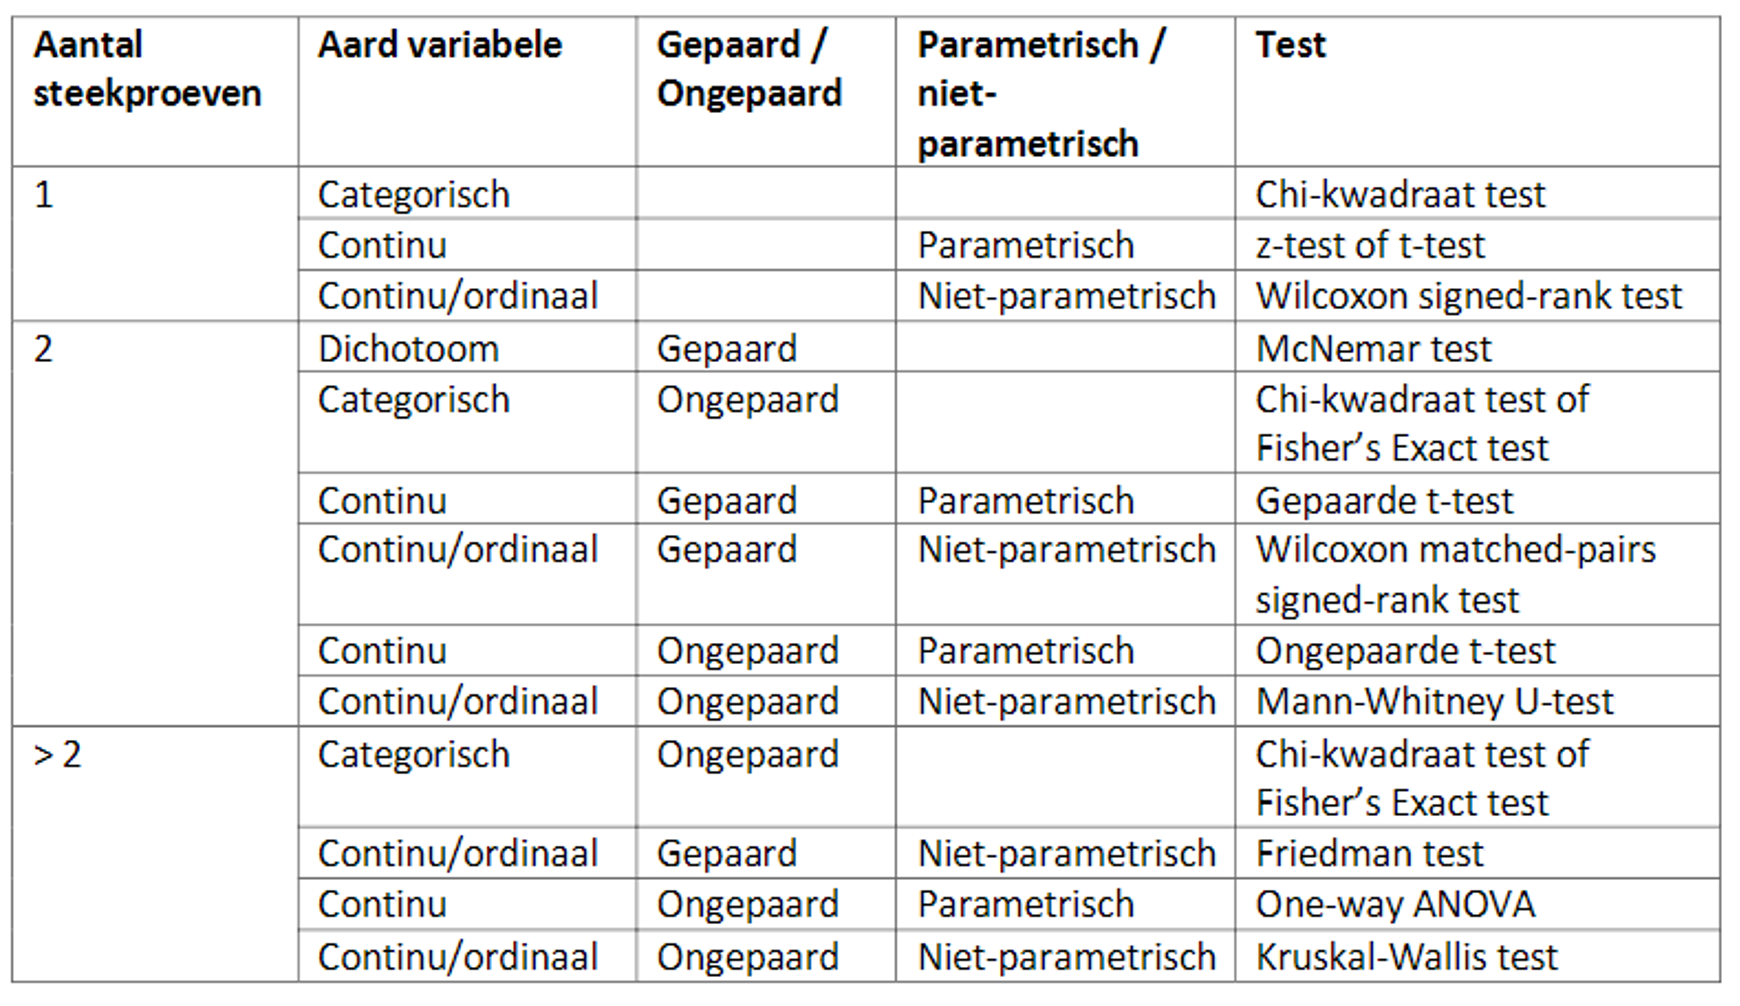
\includegraphics[width=1\linewidth]{img/stat_test} \caption{Keuze van statistische toetsen.}\label{fig:stattest}
\end{figure}

\hypertarget{studie-design}{%
\section*{Studie design}\label{studie-design}}


Er zijn verschillen manieren waarop een studie kan worden uitgevoerd. Bij wijze van voorbeeld nemen we een studie waarbij we 100 sporters includeren (\(n = 100\)) waarbij we willen nagaan of lenigheid een risicofactor kan zijn voor het oplopen van een blessure. Bij een cross-sectionele studie voeren we de volledige studie uit op één tijdspunt, m.a.w. is er geen opvolging voorzien van de sporters. Hierbij is het dus belangrijk om al een idee te hebben van welke sporters een blessure hebben opgelopen en welke niet. In een cross-sectionele strudie zal de onderzoeker dus beslissen om een aantal geblesseerde sporters (\(n = 50\)) en niet geblesseerde sporters (\(n = 50\)) te includeren, waarbij men vaak kiest voor een gelijke verdeling van het aantal sporters per groep. Binnen een cross-sectionele studie is het uiteindelijke doel om de lenigheid van de geblesseerde groep te vergelijken met de lenigheid van de niet-geblesseerde groep. Bij een longitudinale cohorte is er wel een opvolgperiode voorzien. Wanneer we een longitudinale studie uitvoeren, dan includeren we eerst 100 niet-geblesseerde sporters, die we opvolgen voor een specifieke follow-up periode (bijvoorbeeld 1 jaar). Tijdens een eerste testmoment (vaak baseline genoemd) evalueren we de lenigheid bij alle geïncludeerde sporters. Tijdens de opvolgperiode houden we bij welke sporters geblesseerd raken en welke niet. Op het einde van de studie kunnen we de baseline-lenigheid vergelijken tussen sporters die zich al dan niet blesseerden. Elk van deze specifieke studie-designs hebben zowel voordelen als nadelen. Zo staat een longitudinale proscpetieve cohorte hoger aangeschreven in de evidentiepyramide, aangezien er een kleinere kans op confounding is bij deze studies. Anderzijds zijn studies met een opvolgperiode aanzienlijk duurder en moeilijker op uit te voeren.

\hypertarget{epidemiologie}{%
\section*{Epidemiologie}\label{epidemiologie}}


Om een aandoening epidemiologisch te beschrijven bestaan er twee veelgebruikte indicatoren, namelijk de \texttt{incidentie} en \texttt{prevalentie}. De \texttt{prevalentie} is een inschatting van het aantal individuen die op een gedefinieerd tijdspunt lijden aan een bepaalde aandoening. Wanneer we de \texttt{prevalentie} willen bepalen van blessures bij 100 sporters bij de start van 2011, bekijken we het aantal sporters die leiden aan een blessure zoals visueel weergegeven in figuur \ref{fig:incprev}. Hierbij merken we op dat er 5 sporters een blessure hebben en de geschatte prevalentie dus \(\frac{5}{100}\) of \(5\%\) zijn. De \texttt{ìncidentie} is een inschatting van het aantal nieuwe individuen die leiden aan de aandoening over een welgedeifinieerde periode. Een belangrijk verschil met de \texttt{prevalentie} is dat we steeds starten met een groep van sporters die aan het begin van de periode waarbij we de \texttt{incidentie} gaan berekenen. Wanneer we de \texttt{incidentie} willen bepalen van blessures in het jaar 2011 starten we van de groep zonder de aandoening (\(100 - 5 = 95\)). In de groep van 95 sporters zonder blessure, zijn er \(6\) die een blessure hebben opgelopen. De incidentie in 2011 wordt dus geschat op \(\frac{6}{95}\) of 6\(\%\).

Om een inschatting te maken van de \texttt{prevalentie} van een aandoening volstaat informatie over het al dan niet aanwezig zijn van een aandoening op een bepaald tijdstip (cross-sectionele studie). Om een inschatting te maken van de \texttt{incidentie} van een aandoening is een follow-up periode noodzakelijk (prospectieve follow-up cohorte).

\begin{figure}
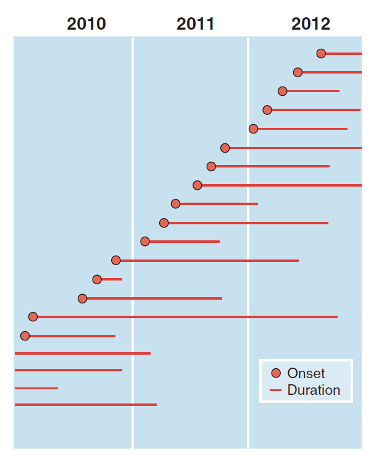
\includegraphics[width=1\linewidth]{img/inc_prev} \caption{Incidentie en prevalentie.}\label{fig:incprev}
\end{figure}

\mainmatter

\hypertarget{corr}{%
\chapter{Correlaties}\label{corr}}

In de paper van Al-Hadidi et al.~(2019) vermeld men volgende stelling:

\begin{quote}
``A significant positive correlation was also found between the duration of use for studying and the duration of pain (p\textless{} 0.001, r = 0.212).''

---Al-Hadidi et al.~(2019)
\end{quote}

\begin{itemize}
\tightlist
\item
  Kunnen we hieruit besluiten dat verhoogd smartphonegebruik de oorzaak is van langdurigere nekpijnervaringen?
\item
  Hoe interpreteren we de \(r\) en \(p\)-waarde? Kunnen we hieruit besluiten dat er een sterke link is?
\end{itemize}

\hypertarget{inleiding}{%
\section*{Inleiding}\label{inleiding}}


Er zijn verschillende manieren om een associatie tussen twee variabelen in te schatten. Eén van de meest gebruikte statistische maten om een verband tussen twee variabelen aan te tonen is een correlatie. Er is er een uitgebreid gamma aan correlaties beschikbaar die gebruikt worden om een verband tussen verschillende specifieke types variabelen aan te tonen. Binnen deze cursus focussen we op correlatiecoëfficiënten die het verband tussen twee \textbf{continue} variabelen trachten in te schatten.

Belangrijk om te onthouden is dat correlaties nooit een oorzaak-gevolg relatie kunnen inschatten binnen een cross-sectionele studie. Oorzaak-gevolg relaties (of causale relaties) kunnen enkel aangetoond worden bij gerandomiseerde studies (vb. RCT). Dit is één van de voornaamste redenen waarom een RCT bovenaan de evidentietabellen terug te vinden is (Figuur \ref{fig:evidenceladder}). Binnen een niet-gerandomiseerde studie kan een schatting van de correlatie vervuild/verstoord zijn door onderliggen de factoren die een belangrijke rol spelen, maar niet in rekening werden gebracht of niet geobserveerd werden.

\begin{figure}
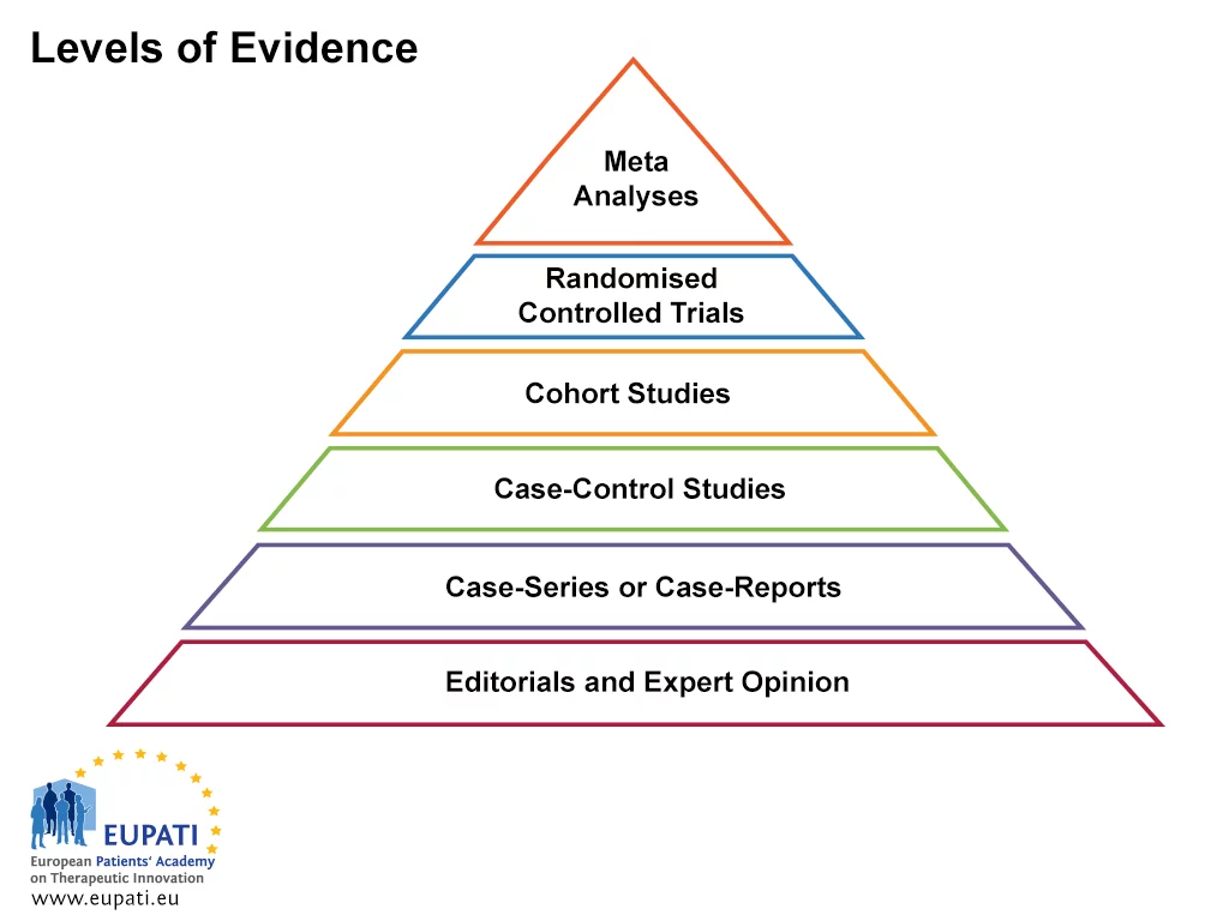
\includegraphics[width=1\linewidth]{img/evidenceladder} \caption{Evidentiepiramide.}\label{fig:evidenceladder}
\end{figure}

Volgend voorbeeld verduidelijkt het probleem van vervuilig van een associatie. In tabel \ref{tab:aggr}, worden de resultaten weergegeven van deze studie. Zoals aangegeven in deze tabel is het slaagpercentage 80\% binnen de groep van mannen en is het slaagpercentage 67\% binnen de groep van vrouwen. Hieruit zouden we kunnen besluiten dat er significant minder vrouwen slagen op een wiskundetoets in vergelijking met mannen.

\begin{table}

\caption{\label{tab:aggr}Scores op wiskundetoets bij studenten na behalen diploma per geslacht.}
\centering
\begin{tabular}[t]{lrr}
\toprule
Gender & Geslaagd & Niet Geslaagd\\
\midrule
Man & 40 & 10\\
Vrouw & 20 & 10\\
\bottomrule
\end{tabular}
\end{table}

Wanneer we echter kijken naar de slaagpercentages per studie-achtergrond (Tabel \ref{tab:aggr}), dan blijkt het slaagpercentage in elke groep hetzelfde te zijn. Binnen de groep van wiskundestudenten slaagt iedereen (100\%) en binnen de groep van studenten met een achtergrond binnen de psychologie slaagt 50\%. De vervuiling van de associatie, waardoor het lijkt dat de slaagpercentages hoger zijn bij mannen in vergelijking met vrouwen, treedt op wanneer we geen rekening houden met de studie-achtergrond van de studenten. Dit is een type-voorbeeld van het optreden van \textbf{confounding} binnen een studie.

\begin{table}

\caption{\label{tab:cond}Scores op wiskundetoets bij studenten na behalen diploma per geslacht en achtergrond.}
\centering
\begin{tabular}[t]{llrr}
\toprule
Faculty & Gender & Geslaagd & Niet Geslaagd\\
\midrule
Wiskunde & Man & 30 & 0\\
Wiskunde & Vrouw & 10 & 0\\
Psychologie & Man & 10 & 10\\
Psychologie & Vrouw & 10 & 10\\
\bottomrule
\end{tabular}
\end{table}

\textbf{Een correlatie} geeft binnen een cross-sectionele studie nooit een causaal verband weer. Er kunnen steeds andere factoren onrechtstreeks betrokken zijn die ertoe leiden dat er een correlatie tussen twee variabelen ontstaat, zonder dat dit verband effectief aanwezig is.

\hypertarget{soorten-correlaties}{%
\section*{Soorten correlaties}\label{soorten-correlaties}}


Een veelgebruikte maat voor het beschrijven van een associatie tussen twee variabelen is een correlatie. Een correlatie is een schatting die de sterkte van het verband weergeeft tussen twee variabelen en de kan variëreren tussen \(-1\) en \(1\) (\(\rho \in [-1, 1]\)). Wanneer een correlatie dicht bij \(0\) ligt, wijst dit om geen associatie tussen twee variabelen, terwijl een correlatie dicht bij \(\pm 1\), wijst op een sterk verband tussen twee variabelen. In dedze cursus worden twee correlaties besproken, de Pearson correlatie coëfficiënt (\(\rho\)) en de Spearman correlatie coëfficiënt (\(r_s\)), die elk een specifiek verband weergeven.

\begin{figure}
\centering
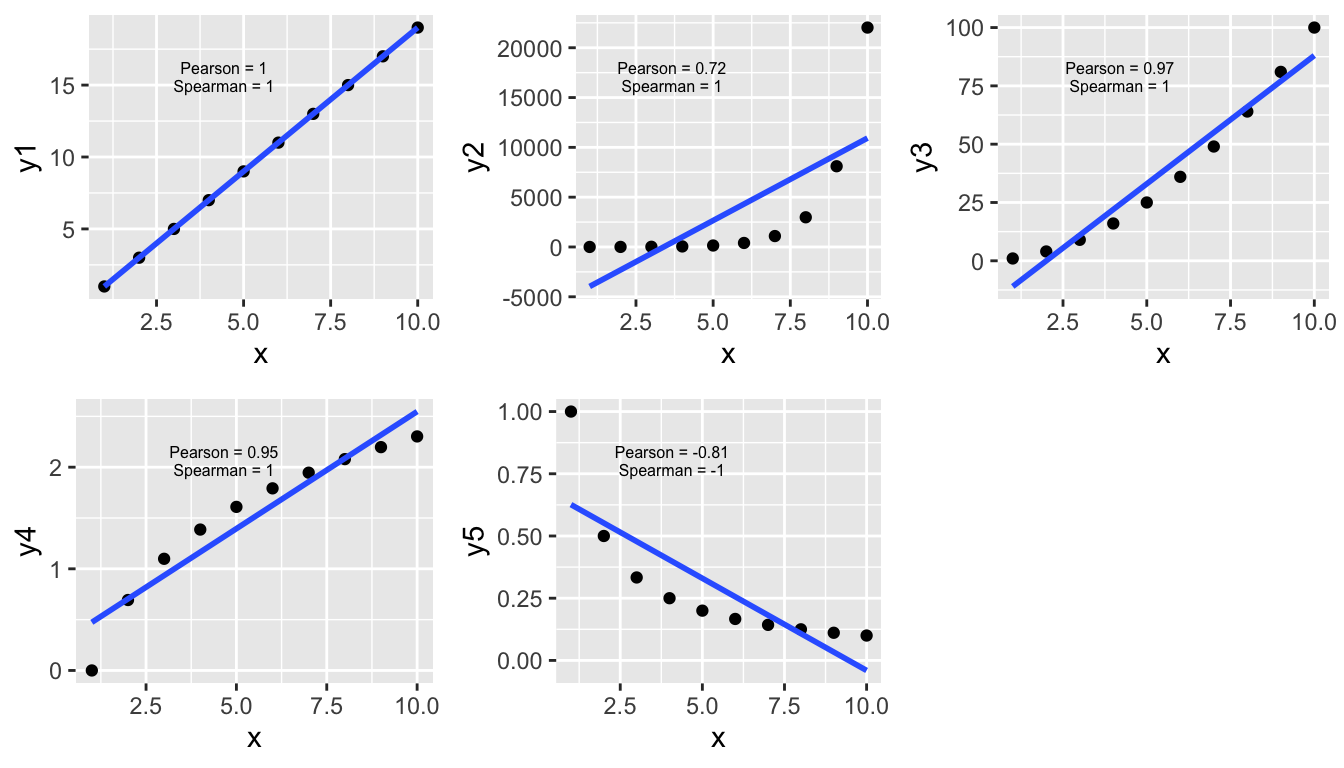
\includegraphics{ugent-ebmstatIII_files/figure-latex/corrs-1.pdf}
\caption{\label{fig:corrs}Different types of associations and their respective correlations}
\end{figure}

In figuur \ref{fig:corrs}, staan een aantal correlaties weergegeven. In deze figuur worden een aantal spreidingsdiagrammen weergegeven waarbij de relatie tussen \(X\) en \(Y\) steeds verschillend is. De punten op de grafiek geven de effectieve waarden weer voor elke observatie, die men kan weergeven als punt (\(x_i\), \(y_i\)). De blauwe lijn op de grafiek geeft steeds de best passende rechte weer door de puntenwolk. Het valt op dat elke Spearman correlatie (\(r_s\)) gelijk is aan 1 of -1 en de Pearson correlatie varieert. Dit fenomeen kan je als volgt interpreteren: een Pearson correlatie het lineaire of rechtlijnige verband nagaat tussen twee variabelen, terwijl de Spearman correlatie nagaat of het om een monotone relatie gaat. Een monotone relatie is een relatie waarbij bij een toename van \(X\), ofwel \(Y\) altijd toeneemt ofwel \(Y\) altijd afneemt. De eerste 4 figuren geven een positief verband weer en ook een positieve correlatie, waarbij een toename in \(X\) samengaat met een toename in \(Y\). De laatste figuur geeft een negatieve relatie weer, waarbij een toename in \(X\) samengaat met een afname in \(Y\).

\begin{table}

\caption{\label{tab:corrtab}Overzicht van karakteristieken en eigenschappen van correlaties.}
\centering
\begin{tabular}[t]{lll}
\toprule
Karakteristieken & Pearson correlatie & Spearman correlatie\\
\midrule
Voorwaarde & Normaal verdeling beide variabelen & Geen\\
Soort relatie & Lineaire relatie & Monotone relatie\\
Mogelijke waarden & {}[-1, 1] & {}[-1, 1]\\
Formule & Gebaseerd op de (co)variantie & Gebaseerd op de rank\\
\bottomrule
\end{tabular}
\end{table}

In tabel @ref(tab: corrtab) staan alle eigenschappen van beide correlatiecoëfficiënten vermeld. De formules voor beide correlaties worden hieronder weergegeven.

\textbf{Interpretatie}: Een correlatie die dichter bij \(1\) of \(-1\) ligt, geeft aan dat er een sterker lineair of monotoon verband is. De observaties liggen in dit geval meer op één lijn. Bij een correlatie \(< 0\) zal bij een toename van \(X\) de waarde van \(Y\) dalen, terwijl bij een correlatie \(> 0\) een toename van \(X\) gelijklopen met een toename \(Y\).

\hypertarget{peason-correlatie-rho}{%
\subsection{\texorpdfstring{Peason correlatie (\(\rho\))}{Peason correlatie (\textbackslash rho)}}\label{peason-correlatie-rho}}

Bij de formule voor \(\rho\), vinden we in de teller kenmerken terug van de formule voor covariantie en in de noemen kenmerken voor de variantie.

\(\rho = \frac{\sum^n_{i=1} (x_i-\bar{x})(y_i-\bar{y})}{\sqrt{\sum^n_{i=1}(x_i-\bar{x})^2} \sqrt{\sum^n_{i=1}(y_i-\bar{y})^2}}\)

\hypertarget{spearman-correlatie-r_s}{%
\subsection{\texorpdfstring{Spearman correlatie (\(r_s\))}{Spearman correlatie (r\_s)}}\label{spearman-correlatie-r_s}}

Bij de formule voor \(r_s\), vinden we in de teller de rang terug van de verschillende correlaties en in de noemen kenmerken voor de steekproefgrootte.

\(r_s = \frac{6 \sum d^2_i}{n(n^2-1)}\)

\hypertarget{studie-naar-tevredenheid}{%
\section*{Studie naar tevredenheid}\label{studie-naar-tevredenheid}}


Gegeven is de volgende dataset \texttt{tevreden} met informatie over een bevraging bij kinesitherapeuten over hun tevredenheid van honoraria.

\begin{itemize}
\tightlist
\item
  \(Y\): tevredenheid (schaal 0-10)
\item
  \(X\): leeftijd (jaren)
\end{itemize}

We beschikken in deze specifieke steekproef over een totaal van 9 observaties (\(n = 9\)).

de dataset ziet er als volgt uit:

\begin{table}

\caption{\label{tab:tevereden}Steekproef naar tevredenheid bij kinesitherapeuten.}
\centering
\begin{tabular}[t]{rr}
\toprule
X & Y\\
\midrule
25 & 8\\
34 & 6\\
34 & 7\\
36 & 5\\
42 & 3\\
\addlinespace
44 & 4\\
45 & 4\\
50 & 2\\
62 & 0\\
\bottomrule
\end{tabular}
\end{table}

Als we de relatie visueel willen weergeven tussen de leeftijd en tevredenheid over de honoraria, kunnen we gebruik maken van een spreidingsdiagram, welk er als volgt uitziet:

\includegraphics{ugent-ebmstatIII_files/figure-latex/unnamed-chunk-4-1.pdf}

De hypothese kunnen we als volgt opstellen:

\begin{itemize}
\tightlist
\item
  \(H_0\): Er is geen correlatie (\(\rho\) of \(r_s\) = 0) tussen de leeftijd van de therapeut en de gegeven tevredenheidsscore.
\item
  \(H_1\): Er is een correlatie (\(\rho\) of \(r_s\)) \(\neq\) 0) tussen de leeftijd van de therapeut en de gegeven tevredenheidsscore.
\end{itemize}

Een significante correlatie, wil dus zeggen significant verschillend van 0. Dit geeft \textbf{geen} indicatie over hoe sterk de relatie is! In figuur \ref{fig:corrmagn} kan je een voorbeeld van een indeling voor de sterkte van correlaties.

\begin{figure}
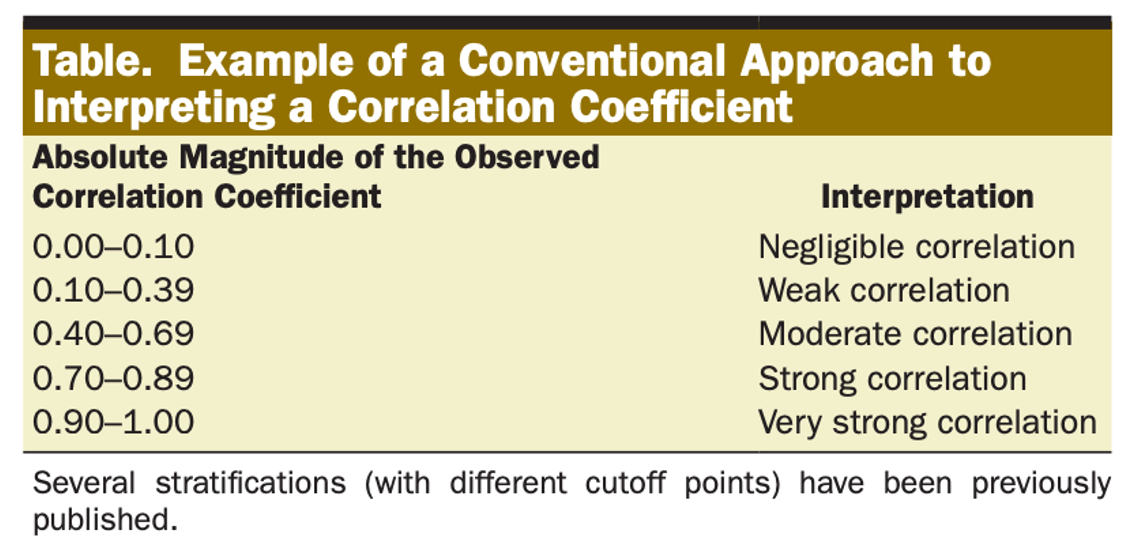
\includegraphics[width=1\linewidth]{img/corr_magn} \caption{Correlatiesterkte}\label{fig:corrmagn}
\end{figure}

\hypertarget{spss}{%
\section*{SPSS}\label{spss}}


In dit hoofdstuk maken we gebruik van de dataset \texttt{tevredenheid}, waarbin \(n=9\) kinesitherapeueten werden bevraagd.

\textbf{Stap 1}: Voer de data in in de \texttt{dataview} van {SPSS}.

\textbf{Stap 2}: Hierna kunnen we de correlaties binnen {SPSS} laten berekenen via \texttt{Analyze\ \textgreater{}\ Correlate\ \textgreater{}\ Bivariate}.

\begin{figure}
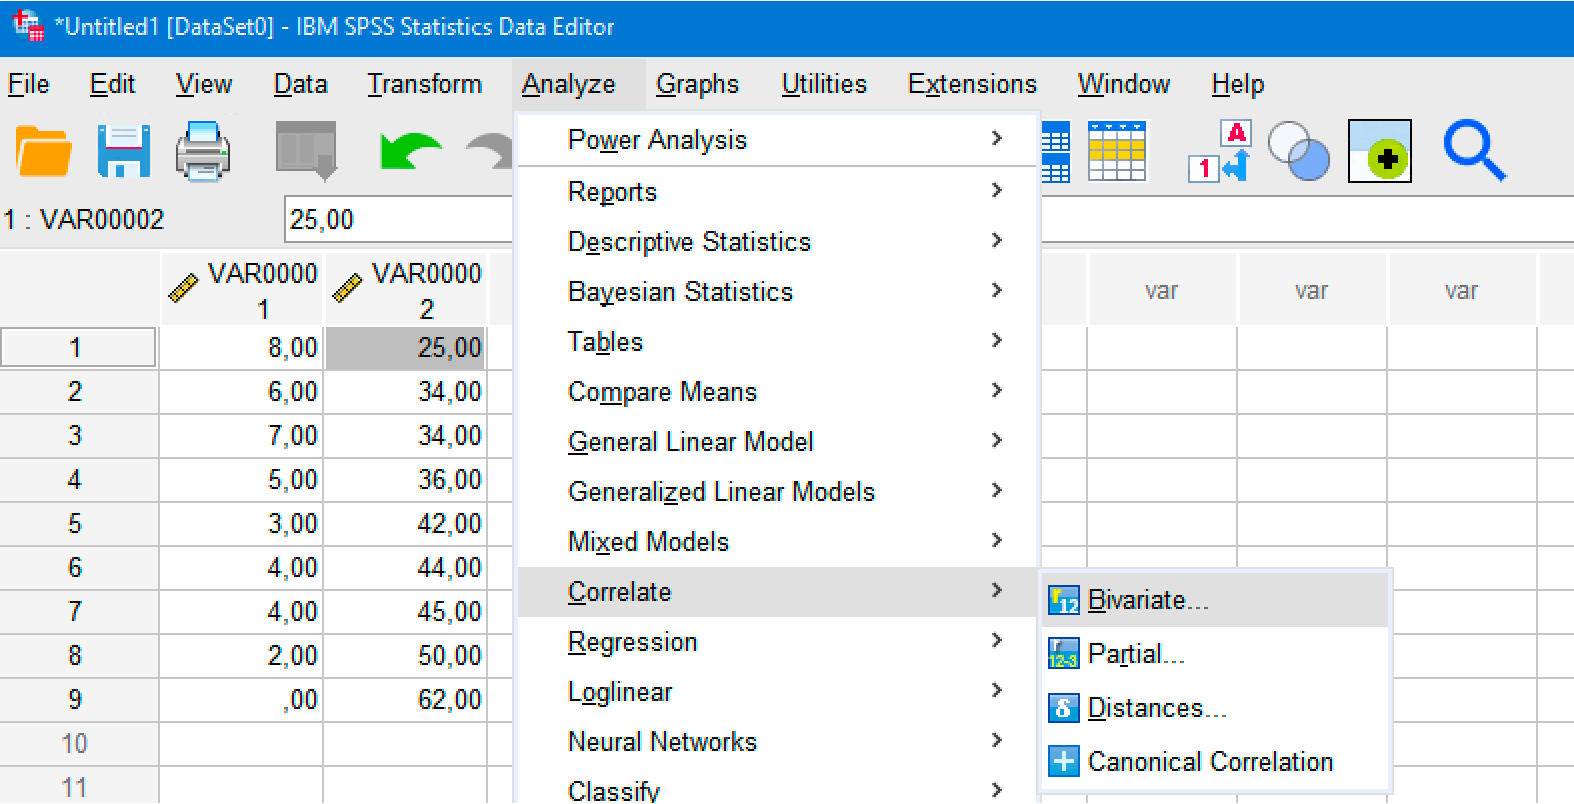
\includegraphics[width=0.75\linewidth]{img/spss_corr_1} \caption{SPSS}\label{fig:corrspss1}
\end{figure}

\textbf{Stap 3}: Hierna krijgen we de pop-up zoals weergegeven in figuur \ref{fig:corrspss2}, waarin we zowel \texttt{Pearson} als \texttt{Spearman} kunnen aanduiden en de verschillend evariabelen waartussen we een correlatie wensen te berekenen. We dienen hierbij minstens 2 variabelen aan de duiden, maar kunnen meerdere variabelen toevoegen. {SPSS} zal automatisch alle 2x2 correlaties berekenen en weergeven in een matrix met op de diagonaal \(\rho = 1\) or \(r_s = 1\).

\begin{figure}
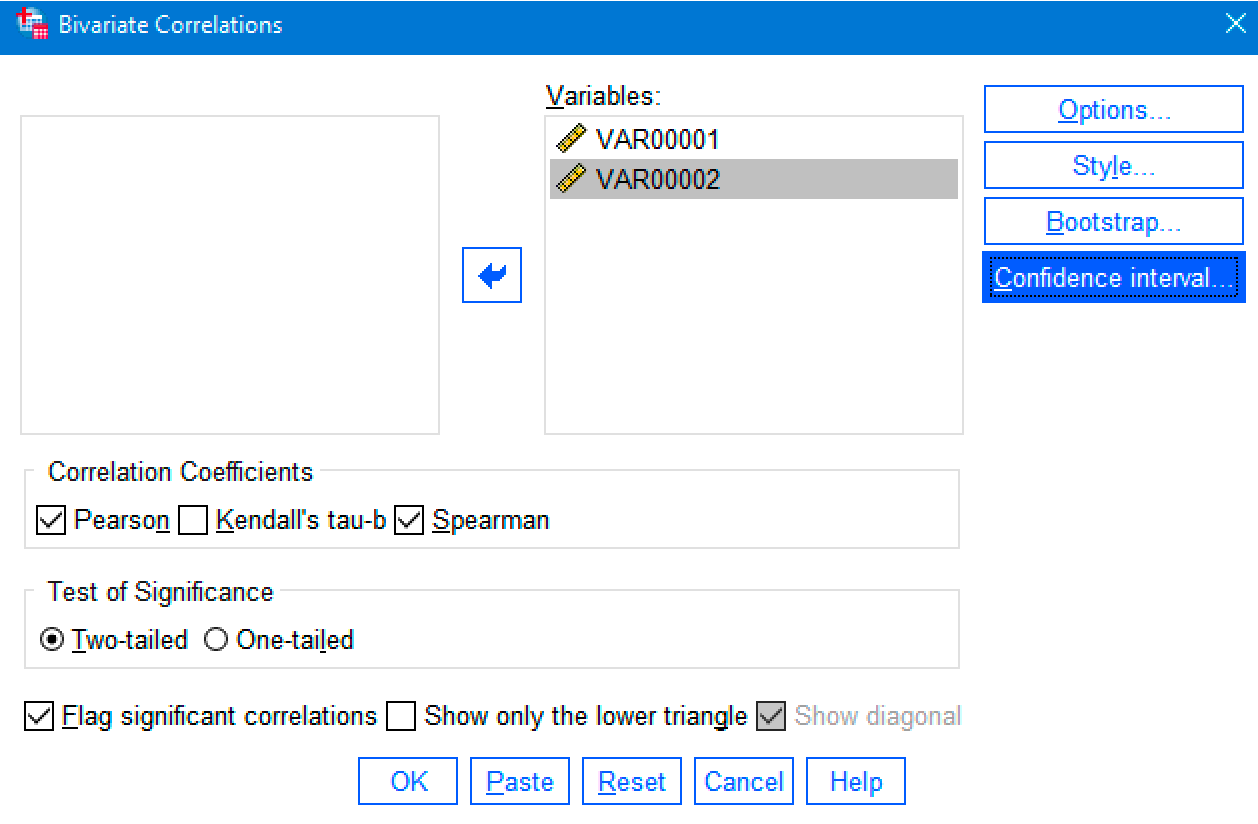
\includegraphics[width=0.75\linewidth]{img/spss_corr_2} \caption{SPSS}\label{fig:corrspss2}
\end{figure}

\textbf{Stap 4}: Vergeet niet om de Syntax te gebruiken binnen {SPSS}.

\begin{figure}
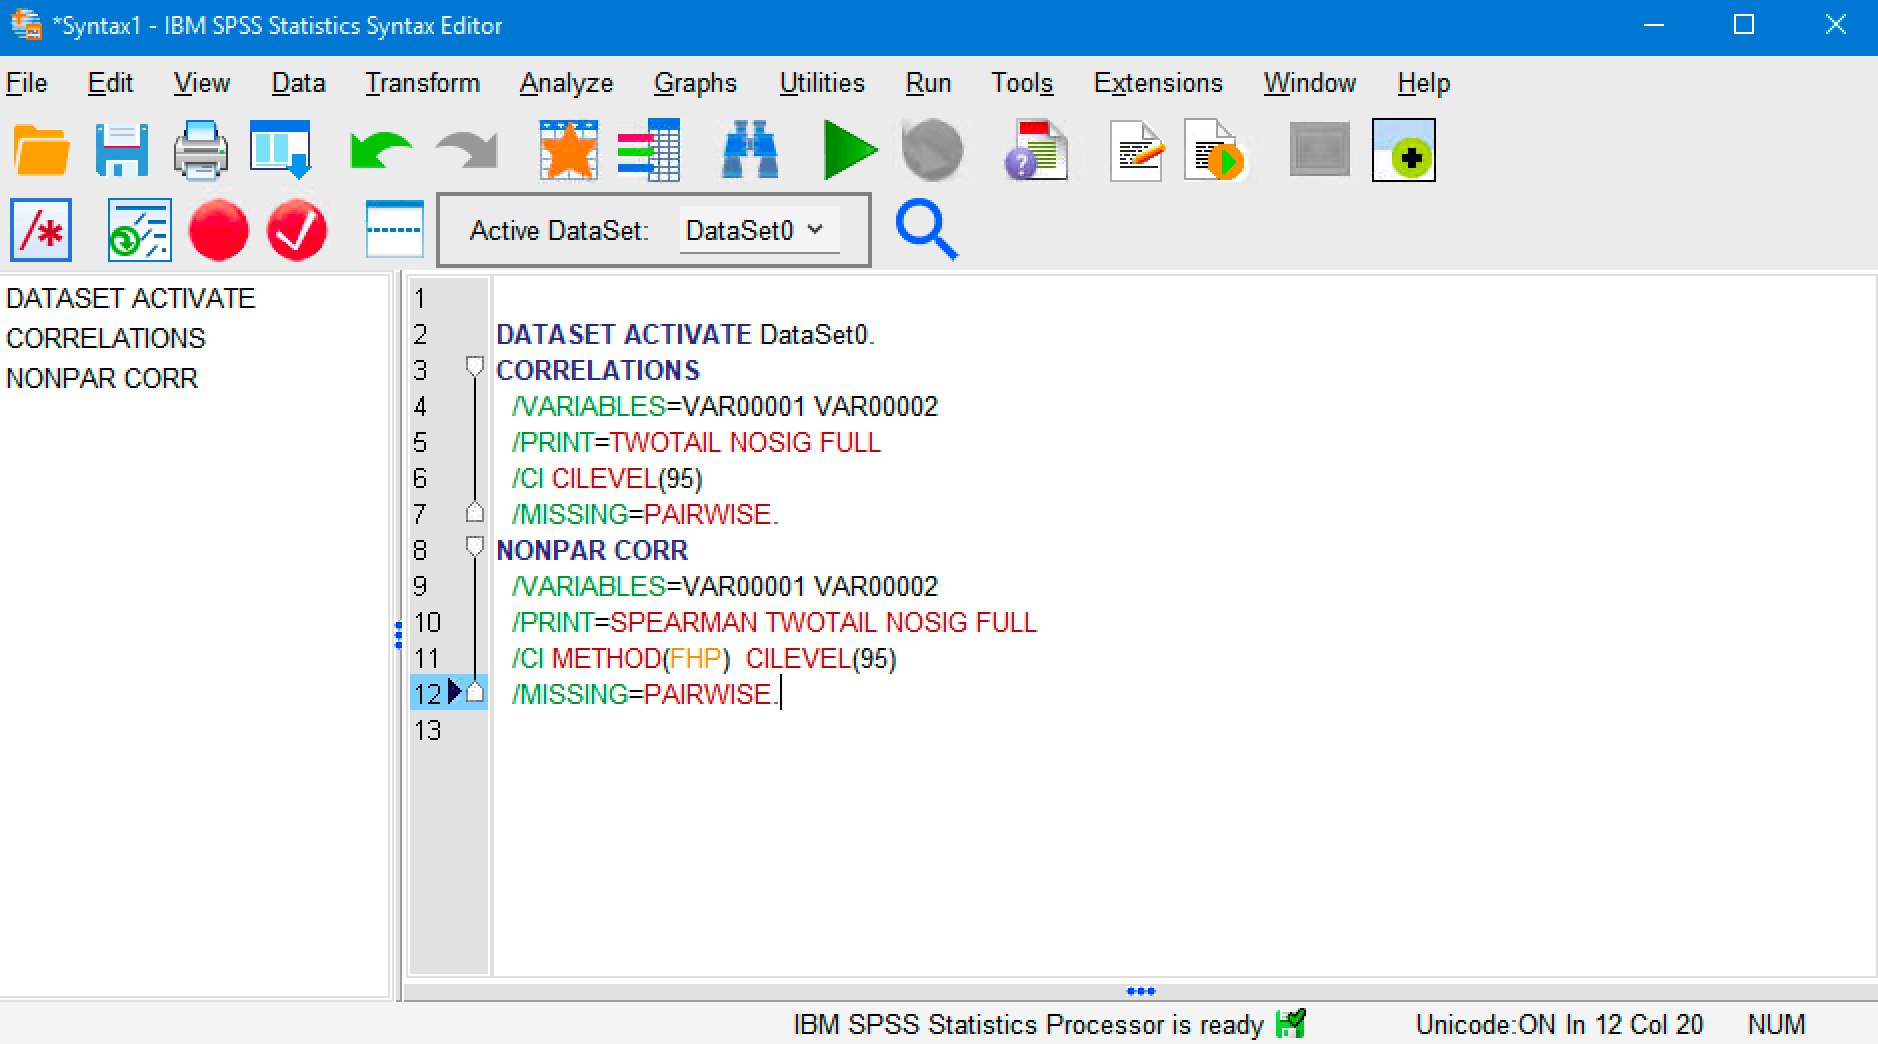
\includegraphics[width=0.75\linewidth]{img/spss_corr_3} \caption{SPSS}\label{fig:corrspss3}
\end{figure}

\textbf{Stap 5}: Tot slot kunnen we de correlaties bekijken en interpreteren. In figuur \ref{fig:corrspss4} vinden we de resultaten voor \(\rho\), terwijl we in figuur \ref{fig:corrspss5} de resultaten voor \(r_s\). We vinden in deze figuren ook de \(p\)-waarde terug en een 95\% betrouwbaarheidsinterval (\(95\% CI\)).

In figuur \ref{fig:corrspss3} zijn de resultaten weergegeven wanneer we de Pearson correlatie berekenen. In figuur \ref{fig:corrspss4} zijn de resultaten weergegeven wanneer we de Spearman correlatie berekenen.

\begin{figure}
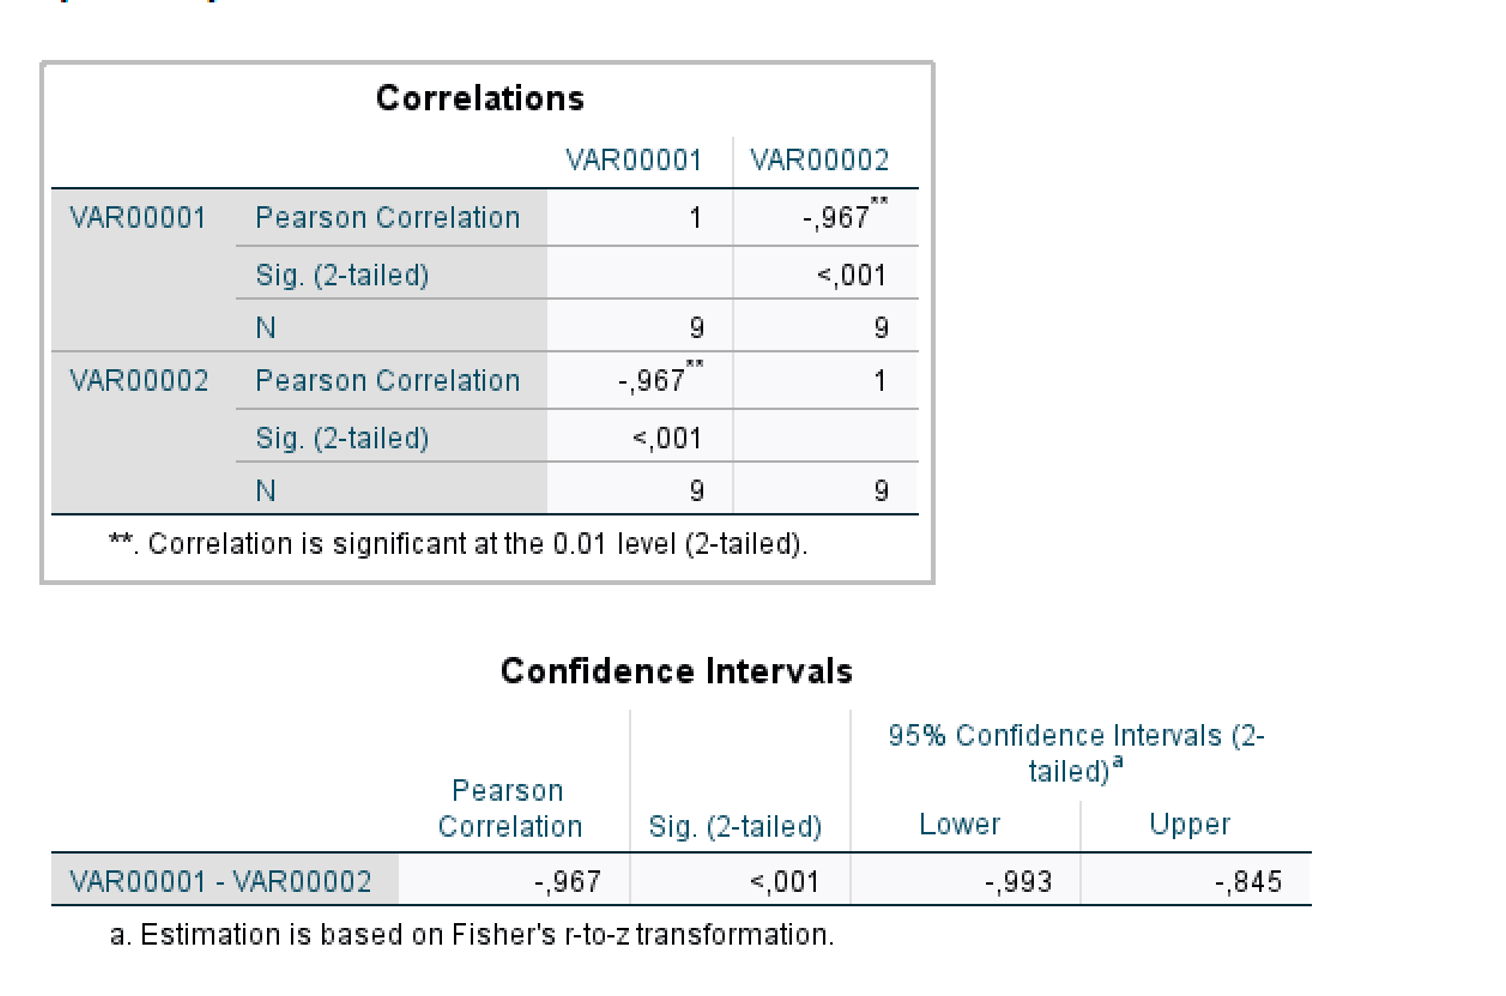
\includegraphics[width=0.75\linewidth]{img/spss_corr_4} \caption{SPSS}\label{fig:corrspss4}
\end{figure}

\begin{figure}
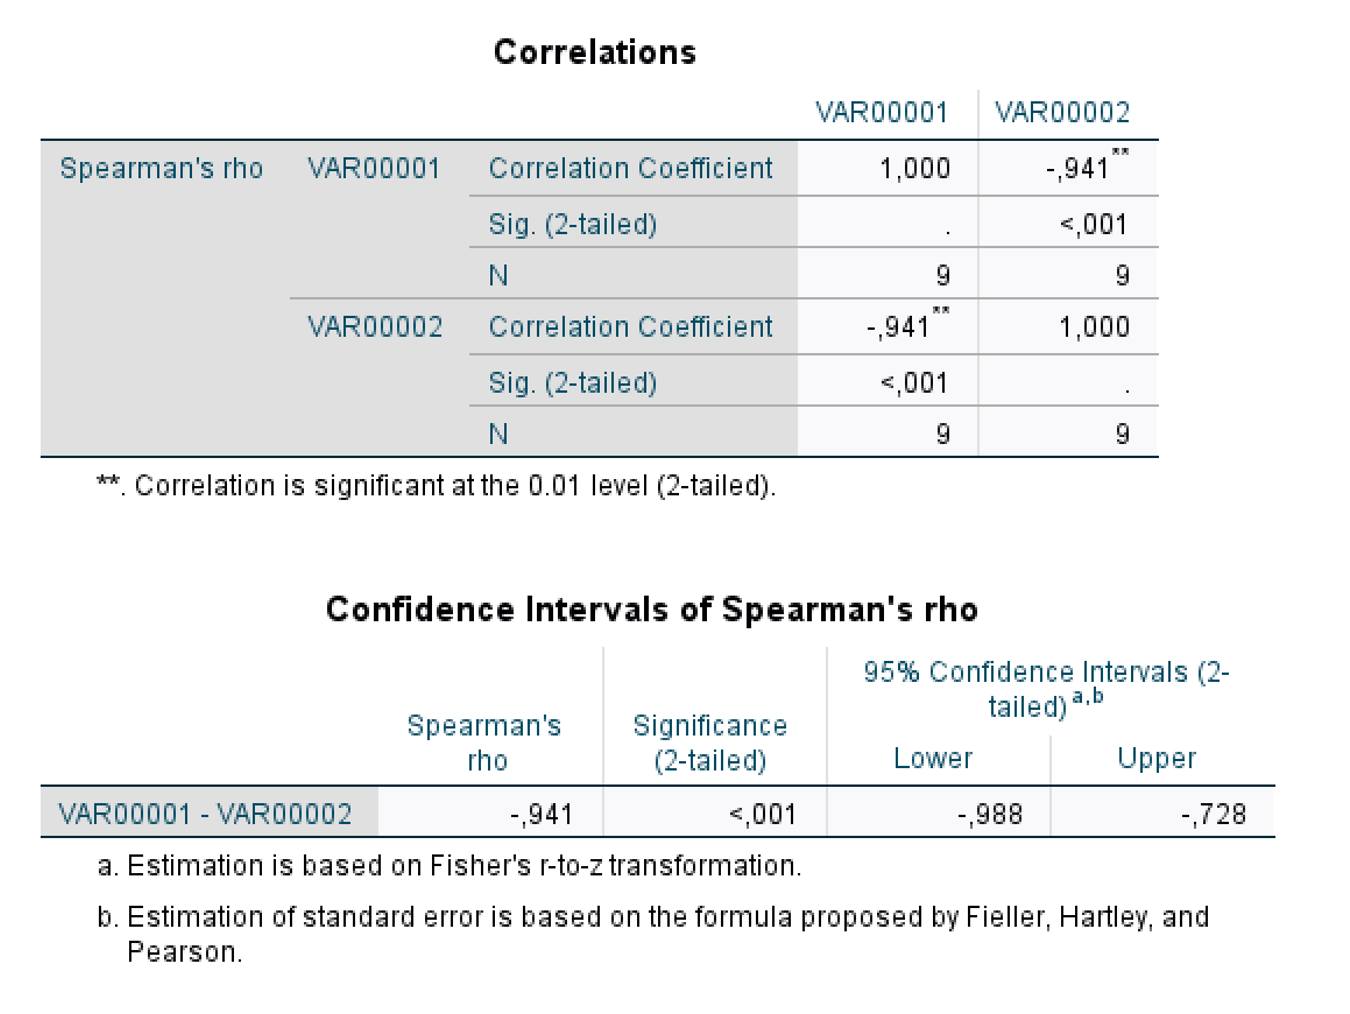
\includegraphics[width=0.75\linewidth]{img/spss_corr_5} \caption{SPSS}\label{fig:corrspss5}
\end{figure}

\newpage

\hypertarget{oefeningen}{%
\section*{Oefeningen}\label{oefeningen}}


In dit onderdeel vinden jullie alle oefeningen over correlaties en associatiaties. De oplossingen worden later gepost op \textbf{Ufora}.

\begin{exercise}

Binnen een onderzoek naar het oplopen van letsel bij sporters, zijn onderzoekers op zoek gegaan naar mogelijke risicofactoren. Ze includeerde 10 sporters, allemaal met een leeftijd van 15 jaar en noteerden de volgende aantal letsels: 5, 0, 0, 2, 2, 3, 1, 2, 1, 0. De onderzoekers waren geïnteresseerd in het verband tussen leeftijd en het aantal letsels. Welke van onderstaande stellingen is WAAR:

\begin{itemize}
\tightlist
\item
  Met een correlatie kunnen we niet aantonen wat een risicofactor is en wat niet.
\item
  We kunnen binnen deze studie geen correlatie berekenen.
\item
  Binnen deze studie kunnen we het verband nagaan tussen aantal letsels en leeftijd door een Pearson correlatie te berekenen.
\item
  Binnen deze studie kunnen we het verband nagaan tussen aantal letsels en leeftijd door een Spearman correlatie te berekenen.
\end{itemize}

\end{exercise}

\begin{exercise}

Een correlatie kunnen we steeds weergeven aan de hand van een lijn.

\begin{itemize}
\tightlist
\item
  Waar
\item
  Onwaar
\end{itemize}

\end{exercise}

De volgende oefeningen zijn gebaseerd op de volgende klinische studie:

\begin{quote}
In een cross-sectionele studie wordt er onderzoek gedaan naar het verband tussen valrisico bij ouderen en de Timed Up and Go (TUG) test. In het totaal zijn er 15 deelnemers binnen de studie waarbij de TUG test wordt afgenomen en de tijd (in s) wordt opgenomen. Verder wordt er bij elke deelnemer ook bevraagd hoevaak ze gevallen zijn het afgelopen jaar.
\end{quote}

In onderstaande tabel \ref{tab:TUG} vinden jullie de resultaten van deze studie. Voer deze gegevens ook in binnen de DATA omgeving van {SPSS} en gebruik het programma waar nodig.

\begin{table}

\caption{\label{tab:TUG}Steekproef naar TUG bij opuderen.}
\centering
\begin{tabular}[t]{rr}
\toprule
Aantal keer gevallen & TUG (s)\\
\midrule
0 & 9.69\\
4 & 17.38\\
2 & 13.87\\
3 & 15.40\\
6 & 21.25\\
\addlinespace
1 & 6.69\\
8 & 22.65\\
1 & 13.79\\
1 & 11.53\\
0 & 14.32\\
\addlinespace
0 & 7.29\\
1 & 10.82\\
1 & 11.95\\
0 & 13.77\\
4 & 20.01\\
\bottomrule
\end{tabular}
\end{table}

\begin{exercise}

Binnen deze studie zullen we kunnen aantonen dat de tijd voor het uitvoeren van de TUG al dan niet een oorzaak is voor meer/minder vallen binnen de oudere populatie.

\begin{itemize}
\tightlist
\item
  Waar
\item
  Onwaar
\end{itemize}

\end{exercise}

\begin{exercise}
Welke grafiek past het best voor een visualisatie van deze gegevens?
\end{exercise}

\begin{exercise}
Welke correlatie zouden jullie selecteren voor het berekenen van een correlatie en waarom?
\end{exercise}

\begin{exercise}
Geef de schatting weer van de door jou geselecteerde correlatiecoëfficiënt tot 2 cijfers na de komma en geef een correcte interpretatie aan deze correlatie.
\end{exercise}

\hypertarget{conclusies}{%
\section*{Conclusies}\label{conclusies}}


\begin{itemize}
\tightlist
\item
  Correlatie \(\neq\) een causaal verband.
\item
  Een correlatie kan gebruikt worden om de sterkte van een lineair \(\rho\) of monotoon \(r_s\) verband uit te drukken.
\item
  De \(p\)-waarde van een correlatie zegt niets over de sterkte van de correlatie.
\end{itemize}

\mainmatter

\hypertarget{regr}{%
\chapter{Lineare regressie}\label{regr}}

In de paper van Chester et al.~(2016) vermeld men volgende stelling:

\begin{quote}
``At 6 weeks only, a better outcome for both measures was associated with no previous compared to a previous major operation (shoulder surgery excluded) (SPADI, \(\beta\) = -3.66 to -12.56).''

---Chester et al.~(2016)
\end{quote}

\begin{itemize}
\tightlist
\item
  Kunnen we hieruit besluiten dat er een statistisch significant verschil is in uitkomst na kinesitherapie tussen patiënten met een vroegere operatie vs geen operatie?
\end{itemize}

In dezelfde studie lezen we:

\begin{quote}
``There was no significant difference in mean age or sex between consenters (57 years, SD = 15, 44\% male) and non-consenters (56 years, SD = 16, 47\% male).''

---Chester et al.~(2016)
\end{quote}

\begin{itemize}
\tightlist
\item
  Kunnen we hieruit besluiten dat er geen baseline verschil is tussen mensen die deelnamen aan de volledige studie vs mensen die vroegtijdig de studie hebben verlaten?
\end{itemize}

\hypertarget{inleiding-1}{%
\section*{Inleiding}\label{inleiding-1}}


Lineaire regressie kan zowel toegepast worden in een cross-sectioneel design als prospectieve cohorte en wordt vaak gebruikt voor volgende doelstellingen:

\begin{itemize}
\tightlist
\item
  Het voorspellen van een uitkomstmaat op basis van één of meerdere factoren.
\item
  Het beschrijven van een verband tussen de uitkomstmaat en andere factoren, waarbij rekening wordt gehouden met verstorende variabelen.
\end{itemize}

In essentie is een lineair regressie model opgebouwd uit twee componenten:

\begin{itemize}
\tightlist
\item
  De afhankelijke uitkomstvariabele (\(Y\)), welke een continue variabele dient te zijn.
\item
  De onafhankelijke variabele(n) (\(X\)), welke zowel continu als categorisch van aard kunnen zijn.
\end{itemize}

\(Y = \beta_0 + \beta_1 X_1 + \epsilon\)

Wanneer er slechts één onafhankelijke variabele \(X_1\) spreken we van een enkelvoudig lineair regressiemodel. Indien er meerdere onafhankelijke variabelen \(X_1, X_2, X_3,..., X_i\) spreken we van een meervoudig lineair regressiemodel.

\textbf{Een regressiemodel} bestaat uit twee delen, een afhankelijk deel (de uitkomst of wat er geschat moet worden) en een onafhankelijk deel (de verklarende variabelen).

\hypertarget{studie-naar-tevredenheid-1}{%
\section*{Studie naar tevredenheid}\label{studie-naar-tevredenheid-1}}


Gegeven is de volgende dataset \texttt{tevreden} met informatie over een bevraging bij kinesitherapeuten over hun tevredenheid van honoraria.

\begin{itemize}
\tightlist
\item
  \(Y\): tevredenheid (schaal 0-10)
\item
  \(X\): leeftijd (jaren)
\item
  \(Z\): geslacht (M/V)
\end{itemize}

We beschikken in deze specifieke steekproef over een totaal van 9 observaties (\(n = 9\)).

de dataset ziet er als volgt uit:

\begin{table}

\caption{\label{tab:tevereden2}Steekproef naar tevredenheid bij kinesitherapeuten.}
\centering
\begin{tabular}[t]{rrl}
\toprule
X & Y & Z\\
\midrule
25 & 8 & M\\
34 & 6 & M\\
34 & 7 & V\\
36 & 5 & V\\
42 & 3 & V\\
\addlinespace
44 & 4 & M\\
45 & 4 & V\\
50 & 2 & V\\
62 & 0 & M\\
\bottomrule
\end{tabular}
\end{table}

Als we de relatie visueel willen weergeven tussen de leeftijd en tevredenheid over de honoraria, kunnen we gebruik maken van een spreidingsdiagram, welk er als volgt uitziet:

\includegraphics{ugent-ebmstatIII_files/figure-latex/unnamed-chunk-7-1.pdf}

Lineaire regressie geeft net als \(\rho\) het lineaire verband weer (in tegenstelling tot \(r_s\), waarbij het monotone verband geschat wordt). Op basis van \(X\) en \(Y\) uit de \texttt{tevreden}dataset werd volgend regressiemodel geschat:

\(Y = 13.6 + (-0.2)X\)

\textbf{Interpretatie}: Wanneer de leeftijd \(X\) toeneemt met één jaar, dan daalt (\(-\)) de tevredenheidscore die gegeven werd door de kinesitherapeuten gemiddeld met 0.2 (\(\beta_1\)). De interpretatie van het getal 13.6 \(\beta_0\) heeft vaak geen reële betekenis. In deze studie geeft de waarde 13.6 weer wat de gemiddelde score zou zijn voor kinesitherapeuten met een leeftijd van 0 jaar.

\includegraphics{ugent-ebmstatIII_files/figure-latex/unnamed-chunk-8-1.pdf}

Op basis van \(Z\) en \(Y\) uit de \texttt{tevreden} dataset werd volgend regressiemodel geschat:

\(Y = 4.2 + 0.3 \times Z\)

\textbf{Interpretatie}: Wanneer we de gemiddelde tevredenheid uitrekenen voor mannen en vrouwen bekomen we volgend resultaat zoals weergegeven in tabel \ref{tab:tevredenmean}. Om tot een numerieke oplossing te komen werden de \texttt{labels} gehercodeerd naar \(0\) voor \(V\) en \(1\) voor \(M\). De waarde van \(\beta_1\) bedraagt nu -0.3, wat het gemiddelde verschil weergeeft tussen mannen en vrouwen voor tevredenheidscore. \(\beta_0\) geeft in dit geval de score weer voor \(Z=0\) (score gegeven door vrouwen).

\begin{table}

\caption{\label{tab:tevredenmean}Gemiddelde tevredenheid bij kinesitherapeuten per geslacht.}
\centering
\begin{tabular}[t]{lr}
\toprule
z & y\\
\midrule
M & 4.5\\
V & 4.2\\
\bottomrule
\end{tabular}
\end{table}

\hypertarget{eigenschappen-van-een-lineair-regressiemodel}{%
\section*{Eigenschappen van een lineair regressiemodel}\label{eigenschappen-van-een-lineair-regressiemodel}}


\hypertarget{schatten-van-lineaire-regressie}{%
\subsection*{Schatten van lineaire regressie}\label{schatten-van-lineaire-regressie}}


Eén van de belangrijste evaluatiecriteria bij een lineair regressiemodel is de meerwaarde van \(X\) in het verklaren van \(Y\). Indien we geen informatie zouden hebben over leeftijd en geslacht, kunnen we \(Y\) het best beschrijven aan de hand van het gemiddelde \(\bar{Y}\).

\includegraphics{ugent-ebmstatIII_files/figure-latex/unnamed-chunk-9-1.pdf}

Om de waarde van de \(X\) variabele in te schatten in het verklaren van \(Y\), kijken we naar de afstand tussen de geschatte regressielijn en de observaties (punten op de grafiek). Wanneer de punten dichter tegen de lijn liggen in vergelijking met een schatting op basis van het algemene gemiddelde \(\bar{Y}\), dan lijkt het dat \(X\) een deel van \(Y\) lijkt te verklaren. Wanneer we \(Y\) willen schatten op basis van de regressielijn, dan duiden we deze schatting aan met \(\hat{Y}\). Zo zal voor \(X = 30\) jaar, \(\hat{Y} = 13.6 + (-0.2)30 = 7.6\).

Het verklaarde deel wordt uitgedrukt als verklaarde variantie. Het becijferen van deze verklaarde variantie gebeurt aan de hand van ANOVA tabellen. Zoals weergegeven in figuur \ref{fig:lmsst} varieert \(Y\) over verschillende waarden. De blauwe bollen geven de observaties weer, terwijl de blauwe horizontale lijn het gemiddelde van \(Y\) weergeeft. De afstand van een observatie (blauwe bol) tot de horizontale lijn, maakt onderdeel uit van de totale variantie. Deze totale variantie wordt ook wel de kwadratensom (Sum of Squares) genoemd. Wiskundig wordt de totale spreiding gedefinieerd als de Total Sum of Squares (SST) ofwel \(\sum ({Y}_i - \bar{Y})^2\). Deze formule geeft aan dat het de som van alle afstanden betreft tussen de blauwe bollen en de blauwe horizontale lijn. Daarnaast hebben we ook de regressielijn of best passende rechte. De afstand van de blauwe bollen tot deze lijn, noemen we de resterende fout van het model of residu (SSE) wat wiskundig \(\sum ({Y}_i - \hat{Y})^2\) word ofwel het verschiul tussen de blauwe bollen en de regressielijn. Tot slot hebben we de verklaarde variantie van het model, welke uitdruk in welke mate het model meer verklaard van de variantie van \(Y\) t.o.v. \(\bar{Y}\). Dit wordt weergegeven door \(\sum (\hat{Y}_i - \bar{Y})^2\).

\begin{figure}
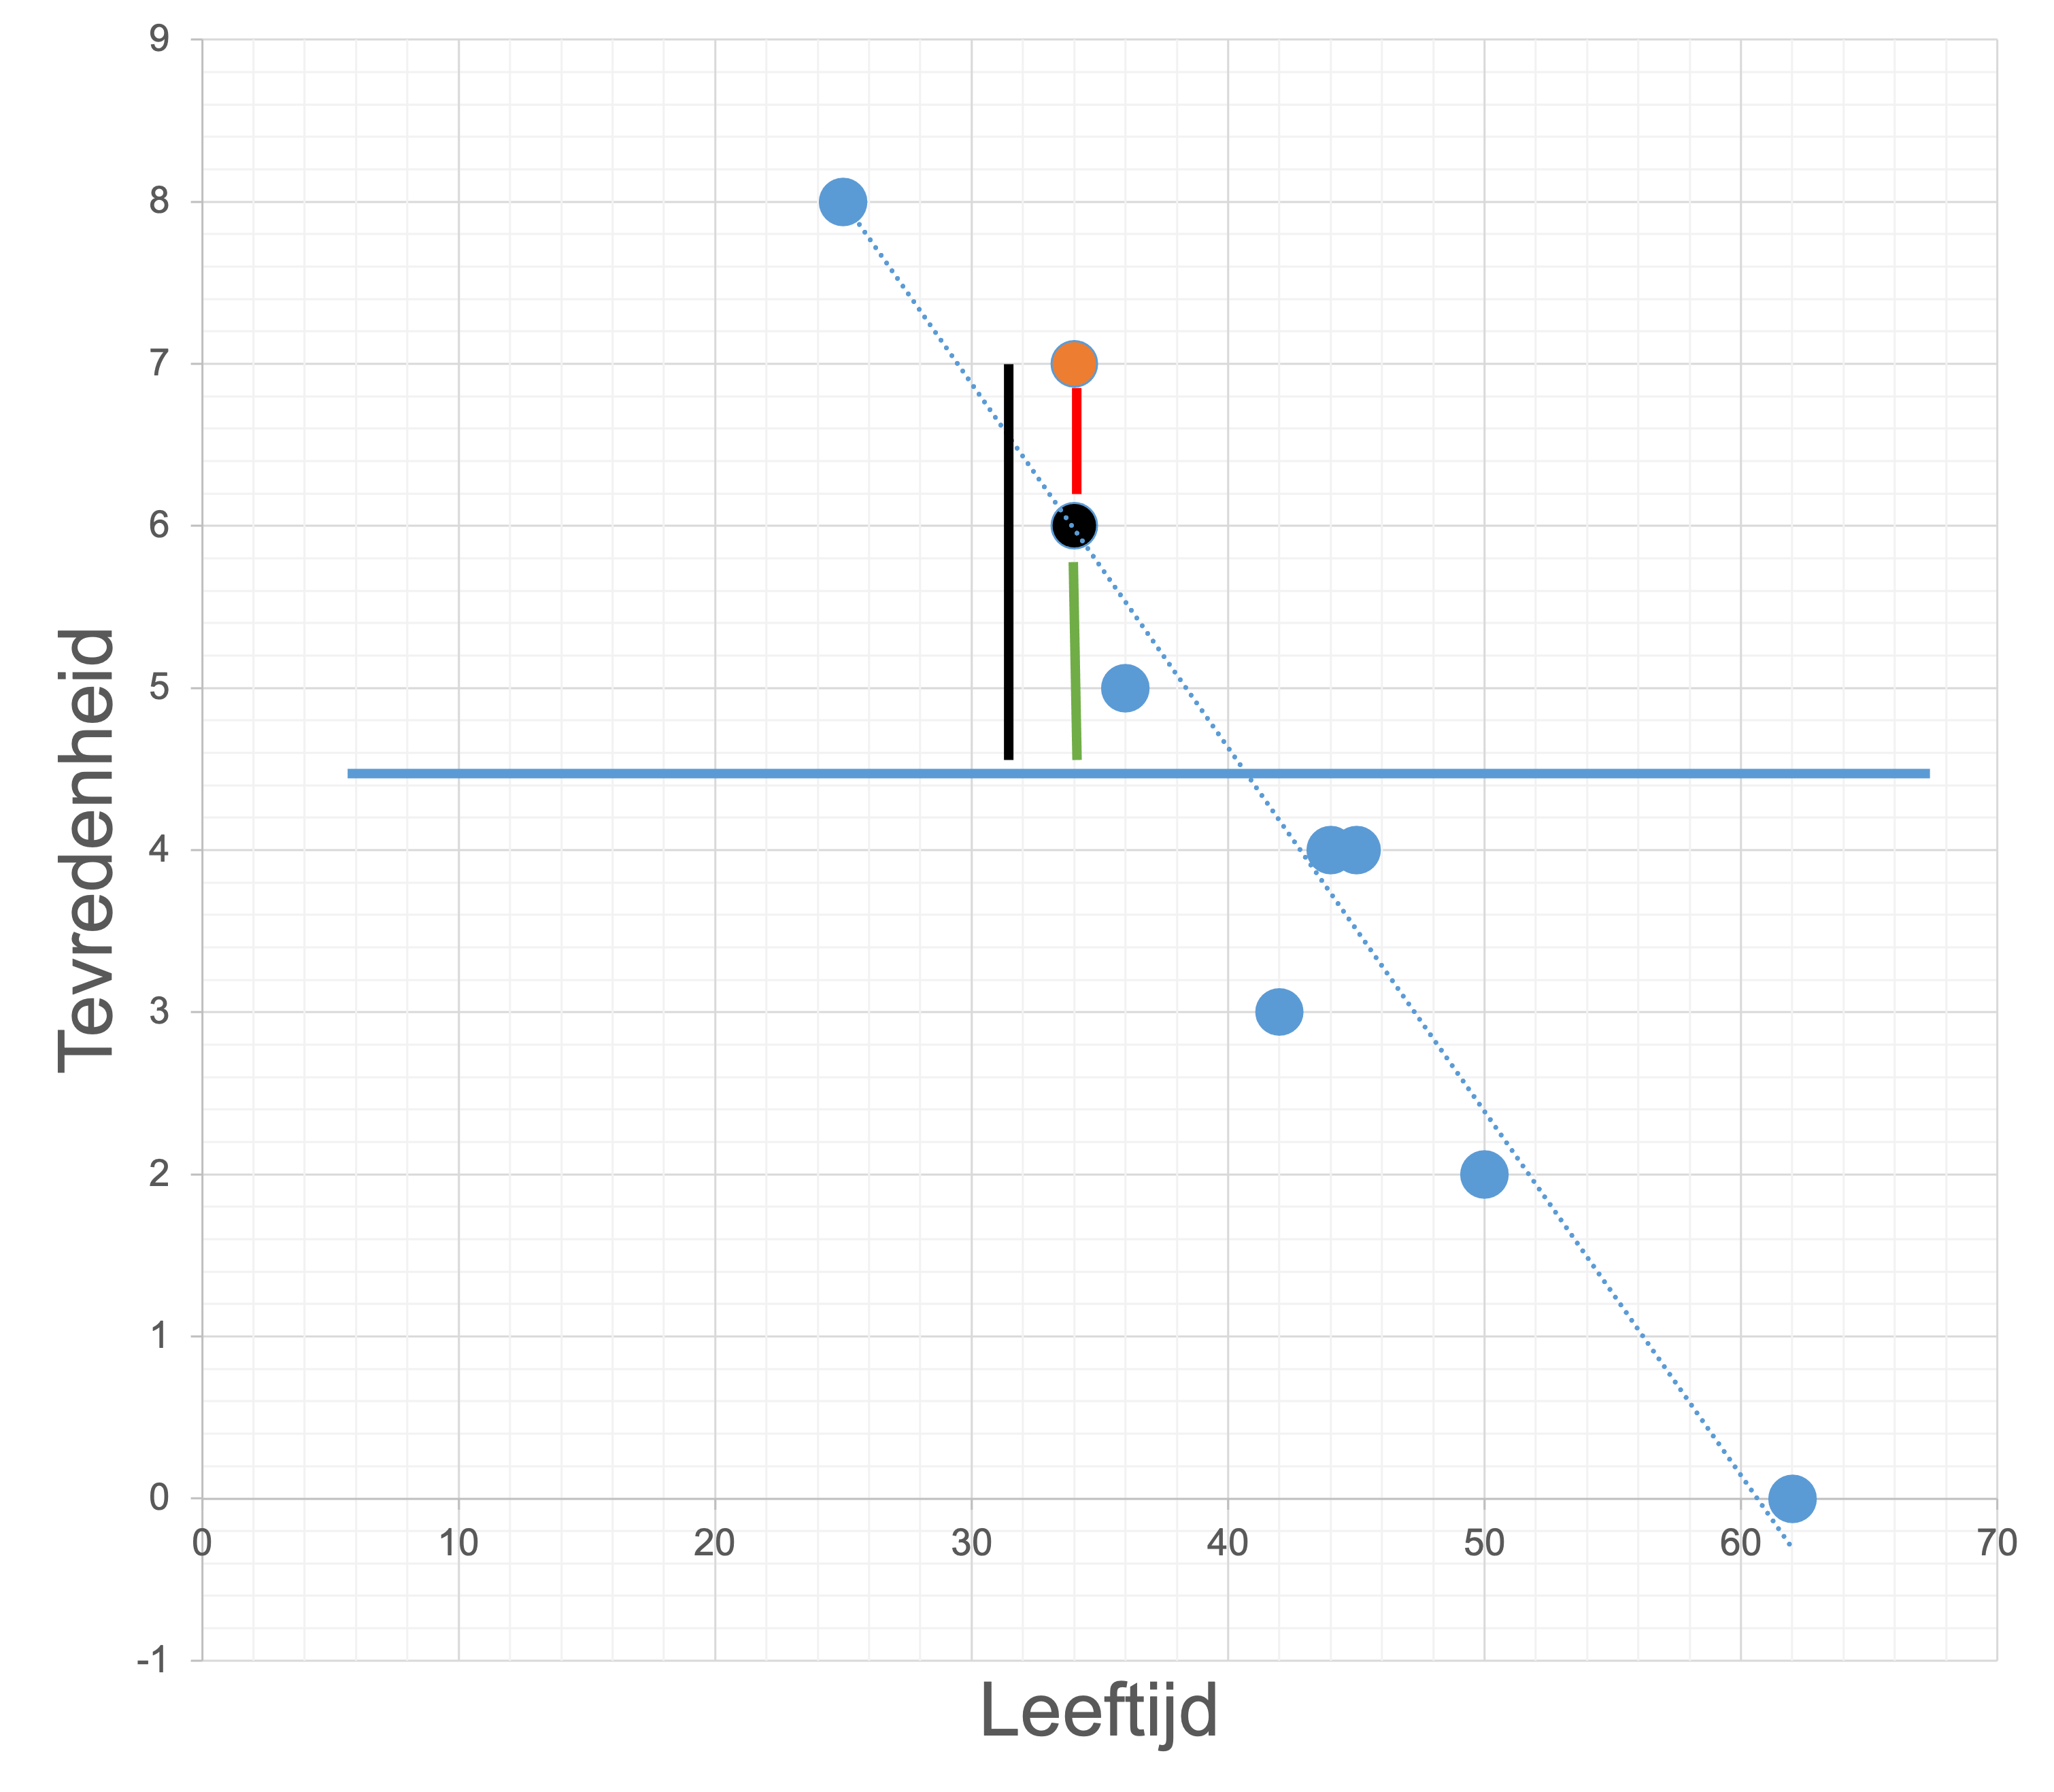
\includegraphics[width=1\linewidth]{img/lm_sst} \caption{Grafische weergave van variantiebronnen}\label{fig:lmsst}
\end{figure}

Uitgewerkt voor de oranje bol (\(X = 34, Y = 7\)) in figuur \ref{fig:lmsst}:

\begin{itemize}
\tightlist
\item
  SST: de afstand tussen de oranje bol \(Y_i\) en de blauwe horizontale lijn \(\bar{Y}\) ofwel \({Y}_i - \bar{Y} = 7 - 4,3 = 2,7\).
\item
  SSE: de afstand tussen de oranje bol \(Y_i\) en de regressielijn \(\hat{Y}\) voor \(X = 34\) ofwel \({Y}_i - \hat{Y} = 7 - (13.6 + (-0.2) \times 34) = 7 - 6 = 1\). (\textbf{opmerking}: hier werden alle cijfers na de komma meegenomen, het volledige model is: \(\beta_0 = 13.6177\) en \(\beta_1 = -0.02246\)).
\item
  SSR: de afstand tussen \(\hat{Y}\) en \(\bar{Y}\).
\end{itemize}

Wanneer we deze oefening voor alles observaties zouden herhalen en kwadrateren en optellen, komen we tot de uiteindelijke kwadratensom.

\begin{table}

\caption{\label{tab:unnamed-chunk-10}Opbouw kwadratensom (1)}
\centering
\begin{tabular}[t]{rrr}
\toprule
SST & SSE & SSR\\
\midrule
3.6666667 & -0.0021598 & 3.6688265\\
1.6666667 & 0.0194384 & 1.6472282\\
2.6666667 & 1.0194384 & 1.6472282\\
0.6666667 & -0.5313175 & 1.1979842\\
-1.3333333 & -1.1835853 & -0.1497480\\
\addlinespace
-0.3333333 & 0.2656587 & -0.5989921\\
-0.3333333 & 0.4902808 & -0.8236141\\
-2.3333333 & -0.3866091 & -1.9467243\\
-4.3333333 & 0.3088553 & -4.6421886\\
\bottomrule
\end{tabular}
\end{table}

Wanneer we al deze waarden kwadrateren komen we tot volgende tabel:

\begin{table}

\caption{\label{tab:unnamed-chunk-11}Opbouw kwadratensom}
\centering
\begin{tabular}[t]{rrr}
\toprule
SST & SSE & SSR\\
\midrule
13.4444444 & 0.0000047 & 13.4602878\\
2.7777778 & 0.0003779 & 2.7133608\\
7.1111111 & 1.0392547 & 2.7133608\\
0.4444444 & 0.2822983 & 1.4351661\\
1.7777778 & 1.4008742 & 0.0224245\\
\addlinespace
0.1111111 & 0.0705746 & 0.3587915\\
0.1111111 & 0.2403752 & 0.6783402\\
5.4444444 & 0.1494666 & 3.7897354\\
18.7777778 & 0.0953916 & 21.5499152\\
\bottomrule
\end{tabular}
\end{table}

Tot slot tellen we alles op:

\begin{table}

\caption{\label{tab:unnamed-chunk-12}Opbouw kwadratensom (3)}
\centering
\begin{tabular}[t]{lr}
\toprule
  & x\\
\midrule
SST & 50.000000\\
SSE & 3.278618\\
SSR & 46.721382\\
\bottomrule
\end{tabular}
\end{table}

Zoals jullie kunnen opmerken uit de laatste tabel, geldt voor de variantiebronnen dat \(SST = SSE + SSR\).

\newpage

\hypertarget{performantie-van-het-regressiemodel}{%
\subsection*{Performantie van het regressiemodel}\label{performantie-van-het-regressiemodel}}


De performantie of verklarende kracht van het regressiemodel wordt uitgedrukt aan de hand van de \emph{determinatiecoëfficiënt} (\(R^2\)). Deze geeft weer hoeveel van de variantie in \(Y\) verklaard kan worden aan de hand van één of meerdere onafhankelijke \(X\) variabelen. Meer bepaald is \(R^2 = \frac{SSR}{SST} = 1 - \frac{SSE}{SST}\). In het voorbeeld hierboven gegeven is \(R^2 = 0.93\) ofwel \(93%
\). De determinatiecoëfficiënt varieerd tussen 0 en 1 (\(R^2 \in [0,1]\)) en hoe dichter bij \(1\), hoe meer van de variantie verklaard kan worden.

Deze berekening wijkt af van de slides door afronding. In de slides werd er geen afronding meegenomen, maar in dit boek werd dit wel meegenomen.

Een volledig overzicht van alle variantiebronnen is weergegeven in onderstaande tabel:

\begin{table}

\caption{\label{tab:unnamed-chunk-13}Overzicht van alle variantiebronnen}
\centering
\begin{tabular}[t]{llll}
\toprule
Bron & Kwadratensom (SS) & Vrijheidsgraden (df) & Kwadratengemiddelde (MS)\\
\midrule
Regressie & \$\textbackslash{}sum ( \textbackslash{}hat\{Y\}\_i - \textbackslash{}bar\{Y\})\textasciicircum{}2\$ & \$m\$ & \$\textbackslash{}frac\{\textbackslash{}sum ( \textbackslash{}hat\{Y\}\_i - \textbackslash{}bar\{Y\})\textasciicircum{}2\}\{m\}\$\\
Residu/Fout & \$\textbackslash{}sum ( Y\_i - \textbackslash{}hat\{Y\})\textasciicircum{}2\$ & \$n-m-1\$ & \$\textbackslash{}frac\{\textbackslash{}sum ( Y\_i - \textbackslash{}hat\{Y\})\textasciicircum{}2\}\{n-m-1\}\$\\
Totaal & \$\textbackslash{}sum ( Y\_i - \textbackslash{}bar\{Y\})\textasciicircum{}2\$ & \$n-1\$ & \$\textbackslash{}frac\{\textbackslash{}sum ( Y\_i - \textbackslash{}bar\{Y\})\textasciicircum{}2\}\{n-1\}\$\\
\bottomrule
\end{tabular}
\end{table}

De uiteindelijke statistische grootheid op basis waarvan de uiteindelijke \(p\)-waarde berekend wordt, is gebaseerd op een afgeleide van de kwadratensom, namelijk het kwadratengemiddelde. Hiervoor wordt elke kwadratensom gedeeld door de bijhorende vrijheidsgraden. Deze vrijheidsgraden zijn \(n-1\) voor de SST (zoals in de formule van variantie uit eerste/tweede Bachelor), \(m\) voor de SSR (waarbij \(m\) het aantal onafhelijke variabelen weergeeft) en \(n-m-1\) voor de SSE. De F-statistiek wordt uiteindelijk berekend als \(F = MS_{regressie}/MS_{residu}\). Hoe groter de waarde van \(F\), hoe meer de regressie in staat is om variantie te verklaren en hoe sneller een statisch signifcant resultaat gevonden kan worden. Voor het \texttt{tevreden} voorbeeld is \(n-1 = 8\), \(m = 1\) en \(n-m-1 = 8-1-1 = 6\). Hieruit kunnen we \(F\) berekenen als \(F = \frac{46.7}{1}/\frac{3.3}{6} = 84.9\)

\begin{figure}
\includegraphics[width=1\linewidth]{ugent-ebmstatIII_files/figure-latex/Ffig-1} \caption{Grafische weergave van variantiebronnen}\label{fig:Ffig}
\end{figure}

Op basis van de berekende \(F\)-waarde en de nul-distributie zoals weergegeven in figuur \ref{fig:Ffig}, zal de \(p\)-waarde \(< 0.001\). Het regressiemodel is met andere waaorden in staat om een significant deel van de variantie van \(Y\) te verklaren op basis van waarden van \(X\).

Bij uitbreiding naar meervoudige lineaire regressie wordt een model als volgt weergegeven: \(Y = \beta_0 + \beta_1X_1 + \beta_2X_2 + … + \epsilon\), waarbij \(Y\) de afhankelijke continue variabele is, \(X_i\) de onafhenkelijke variabele is, \(\beta_i\) een inschatting is van het verband tussen \(X_i\) en \(Y\) en \(\epsilon\) de fout is die gemaakt wordt door het model (\(Y_i - \hat{Y}_i\)).

\hypertarget{hypothesen}{%
\subsection*{Hypothesen}\label{hypothesen}}


Binnen regressie kunnen er twee hypothesen worden opgesteld: (1) een hypothese over de regressie-analyse zelf en (2) een hypothese over de \(\beta\) coëfficiënten. De hypothese kunnen we algemeen als volgt opstellen:

\begin{itemize}
\tightlist
\item
  \(H_0\): Er is geen verband (\(\beta_i = 0\)) tussen de leeftijd (\(X_i\)) van de therapeut en de gegeven tevredenheidsscore (\(Y_i\)).
\item
  \(H_1\): Er is een verband (\(\beta_i \neq 0\)) tussen de leeftijd (\(X_i\)) van de therapeut en de gegeven tevredenheidsscore (\(Y_i\)).
\end{itemize}

Een significante \(\beta_i\) wil dus zeggen significant verschillend van 0 en dus een meerwaarde om iets te zeggen over \(Y\). \textbf{Let op}: binnen deze hypothesen kan het ook over meervoudige regressie gaan met verschillende \(\beta\) coefficiënten.

\(H_0\) kan in dit geval \(\beta_1 = \beta_2 = \beta_3 = 0\) zijn.

Er wordt nooit een hypothese gevormd over \(\beta_0\). Kan je zelf bedenken waarom dit het geval is?

\hypertarget{voorwaarden-van-een-lineair-regressiemodel}{%
\section*{Voorwaarden van een lineair regressiemodel}\label{voorwaarden-van-een-lineair-regressiemodel}}


Er zijn drie belangrijke voorwaarden vooraleer we regressie-analyse kunnen toepassen:

\begin{itemize}
\tightlist
\item
  Lineariteit
\item
  Onafhakelijke waarnemingen
\item
  Residuen normaal verdeeld met gemiddelde 0 en constante variantie
\end{itemize}

De eerste voorwaarde, \textbf{lineariteit}, houdt in dat een regressieanalyse enkel in staat is om een correcte inschatting te maken van een verband tussen één continue afhankelijke variabele en één of meerdere afhankelijke variabelen als dit verband lineair is. Wanneer het verband niet lineair is, zal de inschatting op basis van lineaire regressie een foutief beeld geven, m.a.w. de schattingen zullen niet valide zijn en er zal \emph{bias} optreden.

De tweede voorwaarde, \textbf{onafhakelijke waarnemingen}, geeft aan dat de klassieke lineaire regressie een inschatting kan maken wanneer er slechts één observatie is per variabele per persoon. Indien eenzelfde variabele meerdere malen gemeten of bevraagd werd bij eenzelfde persoon zal de inschatting van de regressie niet correct zijn. De schatting zal nu niet per se onderhevig zijn aan bias, maar de berekeningen van het \(95\% CI\) zal niet correct kunnen gebeuren.

De derde voorwaarde, \textbf{normaal verdeelde residuen}, geeft aan dat de fouten die door het model gemaakt zijn normaal verdeeld moeten zijn met een gemiddelde van 0. Dit is belangrijk aangezien de regressielijn een gemiddelde weergeeft van \(Y\) (\(\bar{Y}\)) voor elke \(X_i\). Indien de residuen niet normaal verdeeld zijn en het gemiddelde van de residuen niet gelijk zou zijn aan 0, gaat de veronderstelling van een gemiddelde inschatting niet meer op.

\hypertarget{selectie-van-een-regressiemodel}{%
\section*{Selectie van een regressiemodel}\label{selectie-van-een-regressiemodel}}


Er bestaan verschillende automatische selectiemethoden om een regressiemodel te definiëren:

\begin{itemize}
\tightlist
\item
  Forward
\item
  Backward
\item
  Enter
\item
  Stepwise
\end{itemize}

In deze cursus gaan we hier niet verder op in.

\hypertarget{dummy-coding}{%
\section*{Dummy coding}\label{dummy-coding}}


Wanneer we gebruik maken van een onafhankelijke categorische \(X\) variabele die bestaat uit \(>2\) cetagoriën, moeten we dummy coding uitvoeren, aangezien we een variabele met bijvoorbeeld 5 categoriën niet kunnen weergeven aan de hand van één \(\beta\) coëfficiënt. Neem bijvoorbeeld tabel \ref{tab:dummy1}, waarbij we de variabele \texttt{Rookstatus} met drie categoriën gaan opdelen in \(m-1\) variabelen, waarbij \(m\) het aantal categoriëen weergeeft. Op basis van rookstatus wensen we in dit voorbeeld een inschatting te maken van het gewicht (in kg).

\textbf{Hier}: \(3-1 = 2\) dummy categoriën.

\begin{table}

\caption{\label{tab:dummy1}Dummy coding}
\centering
\begin{tabular}[t]{lrr}
\toprule
Rookstatus & Actieve roker & Vroegere roker\\
\midrule
Niet roker & 0 & 0\\
Vroegere roker & 0 & 1\\
Actieve roker & 1 & 0\\
\bottomrule
\end{tabular}
\end{table}

Uit tabel \ref{tab:dummy1} kunnen we op basis van slechts twee nieuwe variabelen de drie oorspronkelijke categoriën steeds opnieuw terughalen. Voor elk van deze nieuwe variabelen wordt er in het regressiemodel een \(\beta\) ingeschat. We krijgen hierdoor volgende regressievergelijking:

\(Y = \beta_0 + \beta_1 X_1 + \beta_2 X_2\), waarbij \(X_1\) de associatie is met \texttt{Actieve\ roker} en \(X_2\) de associatie met \texttt{Vroegere\ roker}.

\begin{itemize}
\tightlist
\item
  \(Y = \beta_0 + \beta_1 (actieve \space roker) + \beta_2 (vroegere \space roker)\)
\item
  \(Y = 64 - 2 \times (actieve \space roker) + 0.5 \times (vroegere \space roker)\)
\end{itemize}

Voor een actieve roker komen we dan volgende schatting uit: \(\hat{Y} = 64 - 2 \times (actieve \space roker = 1) + 0.5 \times (vroegere \space roker = 0)\) ofwel \(\hat{Y} = 64 - 2 \times 1 = 62 \space kg\). Voor elk label binnen de variabele \texttt{Rookstatus}, kunnen we dus de inschatting van het gewicht gaan berekenen.

\begin{exercise}
Kan je zelf voor de andere categoriën deze inschatting maken? Hoe bepaal je het gewicht voor de categorie die is weggevallen?
\end{exercise}

Ook in wetenschappelijke artikels zal je binnen categorische variabelen merken dat er aan dummy coding werd gedaan. Hierbij wordt de referentiecategorie vaak gedefinieerd als \(0\).

\begin{figure}
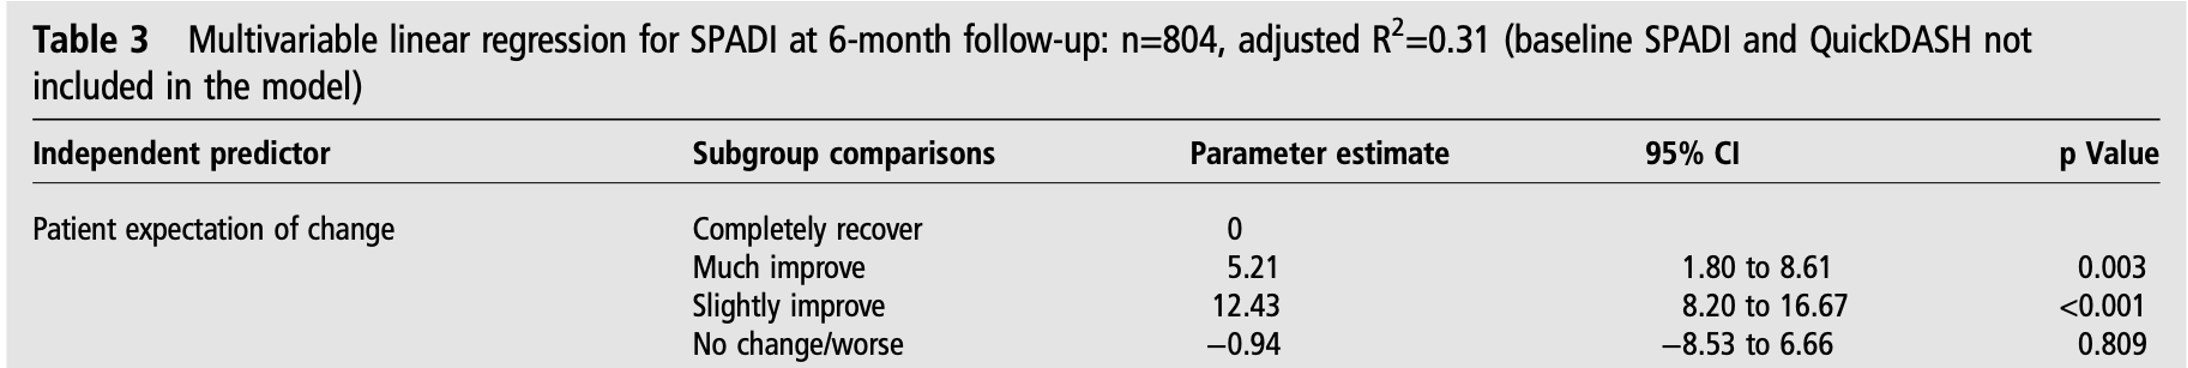
\includegraphics[width=1\linewidth]{img/chester_dummy} \caption{Dummy coding in wetenschappelijk artikel}\label{fig:chesterdummy}
\end{figure}

\hypertarget{multicollineariteit}{%
\section*{Multicollineariteit}\label{multicollineariteit}}


Wanneer we gebruiken maken van meervoudige lineaire regressie, kan er multicollienariteit optreden. Hierbij zijn de verschillende onafhankelijke variabelen onderling gecorreleerd. Multicollienariteit heeft invloed op schatten van de regressiecoëffi¨cnten, betrouwbaarheidsintervallen, etc\ldots{}

Binnen {SPSS} kunnen we hiervoor \texttt{Collinearity\ diagnostics} aanduiden. De twee meest gebruikte schattingen voor collineariteit zijn:

\begin{itemize}
\tightlist
\item
  Tolerance (waarde dicht bij 0 wijst op multicoll.) = \% variantie in de onafh. dat niet kan worden verklaard door de andere onafh. variabelen
\item
  Variance Inflation Factor (VIF) = reciproke waarde van de `Tolerance' (hoge waarde wijst op multicoll.)
\end{itemize}

\hypertarget{spss-en-oefeningen}{%
\section*{SPSS en oefeningen}\label{spss-en-oefeningen}}


In dit deel kunnen jullie voor het eerst kennis maken met lineaire regressie binnen het statistisch softwareprogramma SPSS. Probeer op een gestructureerde manier alle stappen in dit document te volgen en hierna ook de vragen te beantwoorden.

Als kinesitherapeut binnen een obesitaskliniek wil je het verband tussen het BMI (kg/m²) van de patiënten en de uitkomst van de 6-minuten wandeltest (6MWT) in kaart brengen. Gegeven is de volgende dataset:

\begin{table}

\caption{\label{tab:unnamed-chunk-14}Overzicht van data binnen obesitaskliniek}
\centering
\begin{tabular}[t]{rr}
\toprule
BMI (kg/m2) & 6MWT (meter)\\
\midrule
23 & 120\\
28 & 108\\
26 & 105\\
22 & 115\\
31 & 95\\
\addlinespace
26 & 95\\
32 & 82\\
36 & 87\\
42 & 40\\
\bottomrule
\end{tabular}
\end{table}

\begin{exercise}
Bereken de SST voor uitkomst van de 6MWT. Vergeet niet dat de SST berekend wordt door enkel rekening te houden met het gemiddelde.
\end{exercise}

\begin{exercise}
Het verband tussen de 6MWT en het BMI wordt weergegeven aan de hand van volgende formule: \(Y = 195.5 – 3.4X\) OF: \(6MWT = 195.5 – 3.4 \times BMI\) Kan je voorspellen wat de uitkomst op de 6MWT zou zijn voor een person met een BMI van 30?
\end{exercise}

\begin{exercise}
Bereken nu de SSE voor de uitkomst van de 6MWT op basis van bovenstaand regressie-model. Kan je ook de determinatiecoëfficiënt (\(R^2\)) berekenen?
\end{exercise}

Open SPSS en voeg de data in die in de les gebruikt werd voor het beschrijven van het verband tussen de tevredenheid van kinesitherapeuten over hun honoraria en hun leeftijd. Uiteindelijk zou je volgende dataset moeten hebben ingegeven:

\begin{figure}
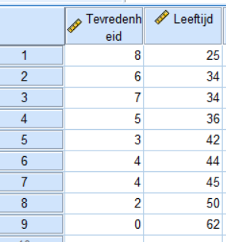
\includegraphics[width=1\linewidth]{img/ex_spss_lm_1} \caption{Data voor tevredenheid}\label{fig:exspsslm1}
\end{figure}

Ga naar \texttt{analyze\ \textgreater{}\ regression\ \ \textgreater{}\ linear} en vul daar volgende gegevens aan:

\begin{figure}
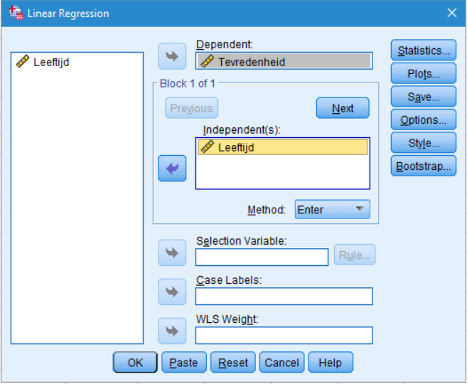
\includegraphics[width=1\linewidth]{img/ex_spss_lm_2} \caption{Model invullen}\label{fig:exspsslm2}
\end{figure}

Let er op dat we tevredenheid onder dependent (afhankelijk) plaatsen en leeftijd onder independent (onafhankelijke). Klik hierna op \texttt{Statistics...} en selecteer onder de statistieken ``confidence intervals''. Klik hierna op \texttt{Paste} en voer de Syntax uit.

\begin{exercise}
Kan je in de output het regressiemodel terugvinden?
\end{exercise}

\begin{exercise}
Is er een significant verband tussen de leeftijd en de score voor tevredenheid? Waaruit leid je dit af?
\end{exercise}

\begin{exercise}
Waarvoor staat het 95\% CI? Kan je dit interpreteren?
\end{exercise}

Open SPSS en voeg de data in die in de les gebruikt werd in oefening 1. Uiteindelijk zou je volgende dataset moeten hebben ingegeven:

\begin{figure}
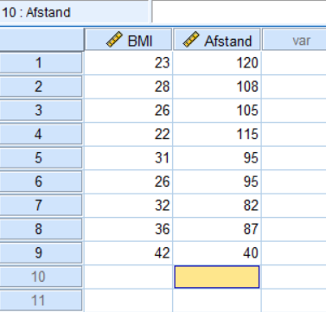
\includegraphics[width=1\linewidth]{img/ex_spss_lm_3} \caption{Data voor obesitas}\label{fig:exspsslm3}
\end{figure}

Ga naar \texttt{analyze\ \textgreater{}\ regression\ \ \textgreater{}\ linear} en vul daar volgende gegevens aan:

\begin{figure}
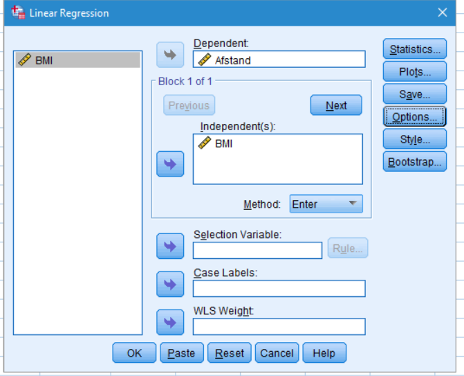
\includegraphics[width=1\linewidth]{img/ex_spss_lm_4} \caption{Model invullen obesaitas}\label{fig:exspsslm4}
\end{figure}

Klik hierna op \texttt{Statistics...} en selecteer onder de statistieken ``confidence intervals''. Klik hierna op \texttt{Paste} en voer de Syntax uit.

\begin{exercise}
Kan je in de output de fouten terugvinden die het model maakt (SSE en SST)? Wat is de waarde van de SSE?
\end{exercise}

\begin{exercise}
Is er een significant verband tussen de BMI en de 6MWT? Wat is de p-waarde voor deze associatie?
\end{exercise}

\begin{exercise}
Waarvoor staat het 95\% CI? Kan je dit interpreteren?
\end{exercise}

Probeer ook nog even volgende meerkeuzevragen te beantwoorden:

\begin{exercise}

Ik heb een categorische variabele over het opleidingsniveau welke bestaat uit 5 mogelijke antwoorden. Selecteer het correcte antwoord.

\begin{itemize}
\tightlist
\item
  Ik kan deze variabele zo toevoegen in het lineaire model in SPSS.
\item
  Ik zal deze moeten hercoderen naar 5 nieuwe variabelen.
\item
  Ik zal deze moeten hercoderen naar 4 nieuwe variabelen.
\item
  Ik zal deze moete hercoderen naar een continue variabele met schaal 1 t.e.m. 5.
\end{itemize}

\end{exercise}

\begin{exercise}

Als ik een lineair model maak in SPSS, dan\ldots{}

\begin{itemize}
\tightlist
\item
  Is het belangrijk dat ik steeds de lineariteit, multicollineariteit en normaalverdeling van de residuen bekijk.
\item
  Dien ik eerst te kijken naar de VIF om multicollineariteit na te gaan.
\item
  Dien ik gebruik te maken van een spearman correlatiecoeffiënt om lineariteit na te gaan.
\end{itemize}

\end{exercise}

\begin{exercise}

Wanneer je verschillende onafhankelijke variabelen hebt, is het vaak moeilijk om een finel model te selecteren. Op basis van jouw opgedane kennis, hoe denk je dat het finaal model het best geselecteerd wordt? Op basis van\ldots{}

\begin{itemize}
\tightlist
\item
  De klinische relevantie.
\item
  Een automatische methode voor variabelen selectie.
\item
  Het veranderen van \(R^2\), hoe hoger deze wordt hoe beter mijn model.
\item
  De significantie van de variabelen in mijn model.
\end{itemize}

\end{exercise}

Je maakt een lineair regressiemodel met extensiekracht ter hoogte van de knie als afhankelijke variabele en leeftijd, lage rugpijn, geslacht en fysieke fitheid als onafhankelijke variabelen. Gegeven is volgende onvolledige ANOVA-tabel. Probeer deze zo goed mogelijk aan te vullen (de zwarte vakken dienen niet te worden aangevuld).

\begin{figure}
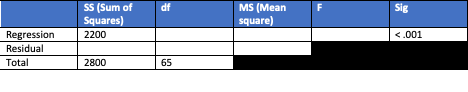
\includegraphics[width=1\linewidth]{img/ex_tab_lm} \caption{Invullen ANOVA tabel}\label{fig:extablm}
\end{figure}

\hypertarget{conclusies-1}{%
\section*{Conclusies}\label{conclusies-1}}


Enkele belangrijke stappen die je steeds moet doornemen:

\begin{itemize}
\tightlist
\item
  ANOVA-tabel en p-waarde
\item
  Determinatiecoëfficiënt (\(R^2\))
\item
  Voorwaarden vervuld (Lineariteit, onafhankelijk en residuen)
\item
  Residuenanalyse
\item
  Klinische relevantie!
\end{itemize}

\begin{itemize}
\tightlist
\item
  Regressie \(\neq\) een causaal verband.
\item
  Regressie is mogelijk met één of meerdere onafhankelijke variabelen.
\item
  De \(R^2\) zegt iets over hoe goed de regressielijn in staat is om \(Y\) te verklaren.
\item
  Regressie geeft steeds een lineair verband weer en is dus gerelateerd aan \(\rho\).
\item
  De afhankelijke variabele \(Y\) bij lieanire regressie is steeds continu.
\end{itemize}

\mainmatter

\hypertarget{logregr}{%
\chapter{Logistische regressie}\label{logregr}}

In de paper van Smith et al.~(2021) vermeld men volgende stelling:

\begin{quote}
``Player age greater than 25 years (OR = 2.9, p \textless{} 0.05), was a factor significantly associated with subsequent hamstring injury.''

---Smith et al.~(2021)
\end{quote}

\begin{itemize}
\tightlist
\item
  Wat kunnen we hieruit besluiten?
\end{itemize}

\hypertarget{risico-relatie}{%
\section*{Risico relatie}\label{risico-relatie}}


Een risico op een aandoening kan vaak ingeschat worden als een kans, waarbij we beroep kunnen doen op de \texttt{prevalentie} en \texttt{incidentie}. Wanneer we weten dat de \texttt{prevalentie} van lage rugpijn 50\% is, dan is binnen de populatie de kans dat iemand lage rugpijn heeft 50\%. De \texttt{prevalentie} (en de \texttt{incidentie}) kan dus gezien worden als een risico op lage rugpijn. Om een risico op een binaire gebeurtenis (waarbij het optreden van bijvoorbeeld lage rugpijn vaak gecodeerd wordt als 1 en het niet optreden van lage rugpijn als 0) statistisch te beschrijven wordt er vaak gebruik gemaakt van twee statistische grootheden, een \texttt{risico} en een \texttt{odds}.

\hypertarget{risico-en-risico-ratio-rr}{%
\subsection*{Risico en risico ratio (RR)}\label{risico-en-risico-ratio-rr}}


Gegeven is de volgende dataset \texttt{tevreden} met informatie over een bevraging bij kinesitherapeuten over hun tevredenheid van honoraria.

\begin{itemize}
\tightlist
\item
  \(Y\): tevredenheid (0-niet tevreden; 1-tevreden)
\item
  \(X\): leeftijd (in categorieën)
\end{itemize}

We beschikken in deze specifieke steekproef over een totaal van 9 observaties (\(n = 10\)).

de dataset ziet er als volgt uit:

\begin{table}

\caption{\label{tab:tevereden3}Steekproef naar tevredenheid bij kinesitherapeuten.}
\centering
\begin{tabular}[t]{lr}
\toprule
X & Y\\
\midrule
< 40 & 1\\
< 40 & 1\\
< 40 & 1\\
< 40 & 1\\
< 40 & 0\\
\addlinespace
< 40 & 0\\
40+ & 0\\
40+ & 0\\
40+ & 0\\
40+ & 1\\
\bottomrule
\end{tabular}
\end{table}

Om het risico op tevredenheid na te gaan (\textbf{risico} kan ook een positieve quotatie hebben), dienen we te identificeren hoeveel indivduen aangegeven hebben tevreden te zijn over hun honorarium. In deze studie gaven 5 van de 10 therapeuten aan tevreden te zijn. Het risico (of kans) op tevredenheid is in dit geval dus 50 \(\%\).

\begin{table}

\caption{\label{tab:teveredenX}Kruistabel van tevredenheid.}
\centering
\begin{tabular}[t]{lrr}
\toprule
  & 0 & 1\\
\midrule
< 40 & 2 & 4\\
40+ & 3 & 1\\
\bottomrule
\end{tabular}
\end{table}

Wanneer we het risico in één groep willen uitzetten ten opzichte van een andere groep, kunnen we gebruik maken van het relatieve risico (of risicoratio).

De risicoratio wordt vaak verkozen boven bijvoorbeeld het risicoverschil, aangezien een klein risico verschil een grote impact kan hebben wanneer het bijvoorbeeld een zeldzame aandoening gaat. Stel dat we het effect van een therapie willen nagaan bij een zeldzame aandoening (waarbij de prevalentie \(2 \%\) is). Wanneer onze therapie in staat is de prevalentie te verlagen naar \(1 \%\), waren we in staat om met onze therapie een verschil te bewerkstelligen van \(1 \%\) (risicoverschil). Als we echter kijken naar de risicoratio (relatief risico), dan waren we in staat om de prevalantie te halveren \(\frac{1\%}{2\%} = 0.5\). Wanneer we dezelfde oefening maken voor een ziekte met een hogere prevalentie (\(50\%\)), dan is een effect van \(1\%\) door therapie nog steeds een effect van \(1\%\), maar het relatieve risico is wel gewijzigd naar \(\frac{49\%}{50\%} = 0.98\). Omwille van deze verschillen wordt er vaak verkozen om risico's te vergelijken op basis van ratio's in plaats van verschillen.

Om het verschil in risico op tevredenheid tussen jongere en oudere therapeuten in te schatten, dienen we eerst het risico op tevredenheid in elke groep te berekenen. Voor de jongste groep \texttt{\textless{}\ 40} is het risico \(\frac{4}{6} = 66.7 \%\), terwijl voor de oudere groep \texttt{40+} het risico \(\frac{1}{4} = 25.0 \%\) is. De risico ratio of relatieve risico (RR) voor tevredenheid in de jongere t.o.v. de oudere groep kan dan geschat worden door \(\frac{0.667}{0.250} = 2.67\). De RR is direct en letterlijk interpreteerbaar als een toegenomen risico op tevredenheid waarbij het risico bij kinesitherapeuten jonger dan 40 jaar 2.6 keer hoger is dan in de groep 40 jaar of ouder.

\hypertarget{odds-en-odds-ratio-or}{%
\subsection*{Odds en odds ratio (OR)}\label{odds-en-odds-ratio-or}}


Om de odds en odds ratio (OR) te berekenen gebruiken we dezelfde dataset:

\begin{table}

\caption{\label{tab:unnamed-chunk-17}Steekproef naar tevredenheid bij kinesitherapeuten.}
\centering
\begin{tabular}[t]{lr}
\toprule
X & Y\\
\midrule
< 40 & 1\\
< 40 & 1\\
< 40 & 1\\
< 40 & 1\\
< 40 & 0\\
\addlinespace
< 40 & 0\\
40+ & 0\\
40+ & 0\\
40+ & 0\\
40+ & 1\\
\bottomrule
\end{tabular}
\end{table}

Om de odds op tevredenheid na te gaan (\textbf{odds} kan ook een positieve quotatie hebben), dienen we te identificeren hoeveel indivduen aangegeven hebben tevreden te zijn over hun honorarium. In deze studie gaven 5 van de 10 therapeuten aan tevreden te zijn. Het risico (of kans) op tevredenheid is in dit geval dus 50 \(\%\). De odds is de verhouding van de kans op het plaatsvinden van een gebeurtenis over de kans dat de gebeurtenis niet plaats vind. De odds wordt berekend door \(\frac{p}{1-p}\) of \(\frac{0.5}{1-0.5} = 1\). De odds op tevredenheid is in dit voorbeeld is dus \(1\), aangezien de kans op een tevreden kinesitherapeut even groot is als de kans op een ontevreden kinesitherapeut.

\begin{table}

\caption{\label{tab:unnamed-chunk-18}Kruistabel van tevredenheid.}
\centering
\begin{tabular}[t]{lrr}
\toprule
  & 0 & 1\\
\midrule
< 40 & 2 & 4\\
40+ & 3 & 1\\
\bottomrule
\end{tabular}
\end{table}

Wanneer we de odds in één groep willen uitzetten ten opzichte van een andere groep, kunnen we gebruik maken van de relatieve odds (of odds ratio). Om de OR op tevredenheid van jongere t.o.v. oudere therapeuten in te schatten, dienen we eerst de odds op tevredenheid in elke groep te berekenen. Voor de jongste groep \texttt{\textless{}\ 40} is de odds \(\frac{4/6}{2/6} = \frac{4}{2} = 2.00\), terwijl voor de oudere groep \texttt{40+} de odds \(\frac{1/4}{3/4} = \frac{1}{3} = 0.33\) is. De odds ratio (OR) voor tevredenheid in de jongere t.o.v. de oudere groep kan dan geschat worden door \(\frac{2.00}{0.33} = 6.1\). De OR is moeilijk en niet letterlijk interpreteerbaar aangezien het weergeeft dat de odds bij kinesitherapeuten jonger dan 40 jaar 6.1 keer hoger zijn dan in de groep 40 jaar of ouder.

\hypertarget{odds-vs-risico}{%
\subsection*{Odds vs Risico}\label{odds-vs-risico}}


De OR geeft is stabiel en verondersteld geen oorzaak-gevolg relatie, terwijl de RR verandert wanneer rijen en kollomen (oorzaak-gevolg) verwisseld worden.

\hypertarget{hypothese-en-sterkte-risico-relatie}{%
\subsection*{Hypothese en sterkte risico-relatie}\label{hypothese-en-sterkte-risico-relatie}}


De hypothese van een OR of RR wordt als volgt geformuleerd:

\(H_0\): Leeftijd is geen risicofactor (RR of OR \(=\) 1) gerelateerd aan de tevredenheid van de therapeut. \(H_1\): Leeftijd is geen risicofactor (RR of OR \(\neq\) 1) gerelateerd aan de tevredenheid van de therapeut.

Een significante risicofactor, wil dus zeggen significant verschillend van 1. Belangrijk om te vermelden is dat een OR (of een RR) \(>\) 1 een hoger risico inhoudt ten opzichte van de referentiecategorie. Een OR (of een RR) \(<\) 1 houdt een lager risico in ten opzichte van de referentiecategorie. Alle ORs (of RRs) groter dan (kleiner dan) één kunnen onderling vergeleken worden qua grootte, maar RRs (of ORs) groter dan één kunnen niet vergeleken met RRs (of ORs) kleiner dan één. Wanneer we de odds ratio's berekenen van risicofactoren voor blessures bij sporters, vinden we een \(OR_{geslacht:man} = 2\) en een \(OR_{geen \space opwarming} = 8\), dan kunnen we besluiten dat het risico gerelateerd aan een opwarming groter is dan het risico gerelateerd aan geslacht, aangezien \(8 > 2\).

We kunnen de referentiecategorie omdraaien voor een OR of RR door de inverse te berekenen (vb. \(\frac{1}{OR}\) of \(\frac{1}{RR}\)). Zo kan de OR voor geen opwarming versus een opwarming gelijk zijn aan 8 (\(OR_{geen \space opwarming} = 8\)), dan is de OR voor een opwarming tegenover geen opwarming: \(OR_{opwarming} = \frac{1}{8} = 0.125\). Deze nieuwe OR is zoals in voorgaand voorbeeld moeilijk te vergelijken met de \(OR_{geslacht:man} = 2\), aangezien \(0.125 < 2\), maar het risico gerelateerd aan opwarming aanzienlijk groter is.

De odds, OR en RR wordt vaak weergegeven na een log-bewerking (met het natuurlijke logaritme: ln). Deze worden dan de log(odds), log(OR) or log(RR), aangezien we door deze transformatie een normaal verdeling van de uitkomst kunnen krijgen.

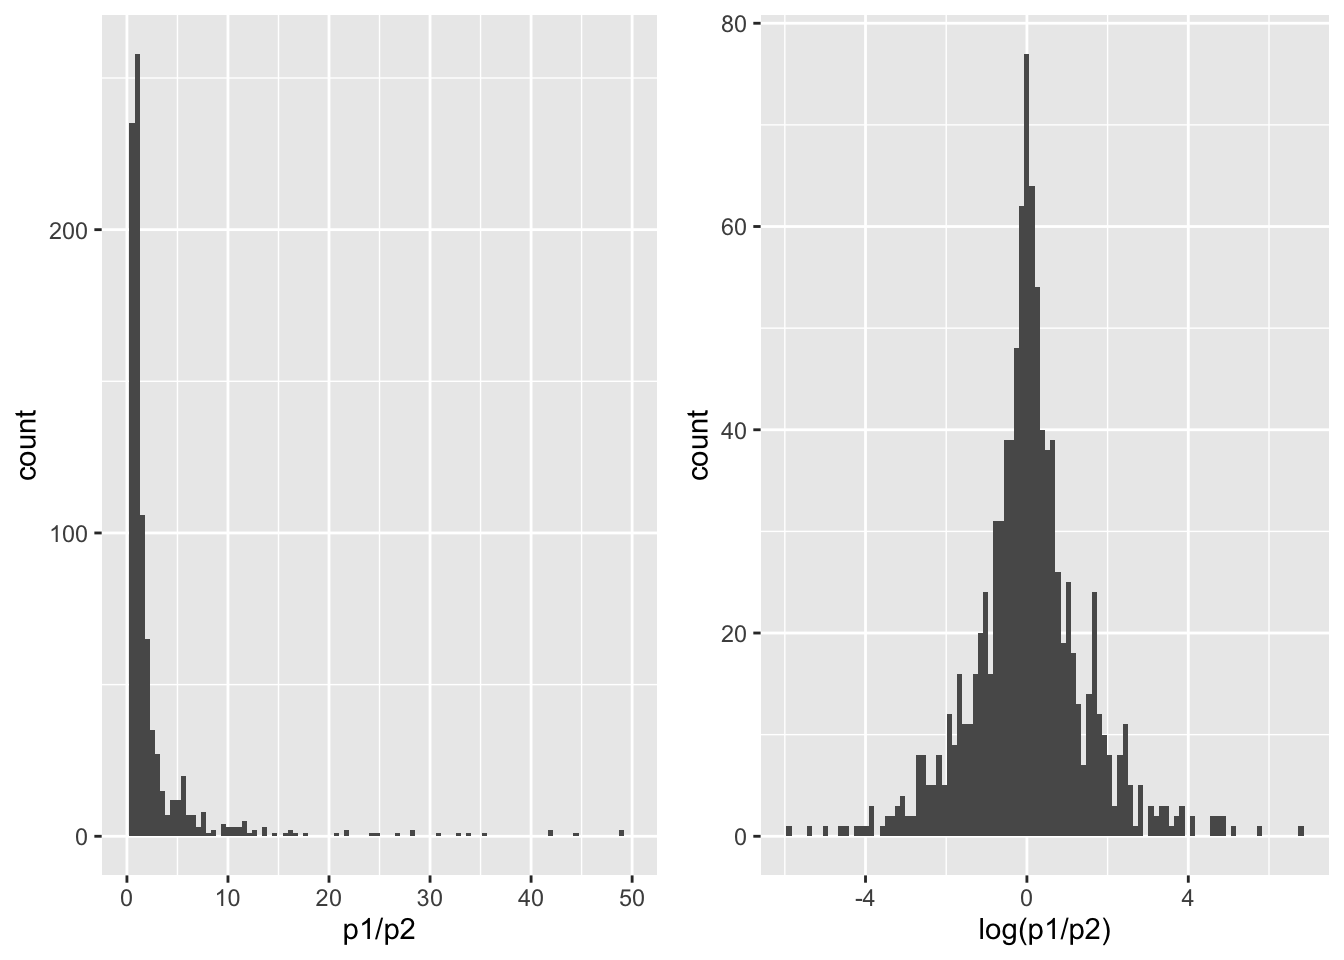
\includegraphics{ugent-ebmstatIII_files/figure-latex/unnamed-chunk-19-1.pdf}

\hypertarget{inleiding-logistische-regressie}{%
\section*{Inleiding logistische regressie}\label{inleiding-logistische-regressie}}


Binaire logistische regressie kan zowel toegepast worden in een cross-sectioneel design als prospectieve cohorte en wordt vaak gebruikt voor volgende doelstellingen:

\begin{itemize}
\tightlist
\item
  Het voorspellen van een uitkomstmaat op basis van één of meerdere factoren.
\item
  Het beschrijven van een verband tussen de uitkomstmaat en andere factoren, waarbij rekening wordt gehouden met verstorende variabelen.
\end{itemize}

In essentie is een logistisch regressie model opgebouwd uit twee componenten:

\begin{itemize}
\tightlist
\item
  De afhankelijke uitkomstvariabele (\(Y\)), welke een categorische variabele dient te zijn.
\item
  De onafhankelijke variabele(n) (\(X\)), welke zowel continu als categorisch van aard kunnen zijn.
\end{itemize}

In de regressievergelijking wordt \(Y\) niet rechtstreeks gemodelleerd, maar de kans op het optreden van \(Y = 1\), welke uitgedrukt wordt als \(p = P(Y=1)\).

\(logit(p) = \beta_0 + \beta_1 X_1\)

Wanneer er slechts één onafhankelijke variabele \(X_1\) spreken we van een enkelvoudig binair logistisch regressiemodel. Indien er meerdere onafhankelijke variabelen \(X_1, X_2, X_3,..., X_i\) spreken we van een meervoudig binair logistisch regressiemodel.

\textbf{Een regressiemodel} bestaat uit twee delen, een afhankelijk deel (de uitkomst of wat er geschat moet worden) en een onafhankelijk deel (de verklarende variabelen).

De logit-functie komt overeen met de log-odds: \(logit(p) = log(odds) = log(\frac{p}{1-p})\).

\hypertarget{studie-naar-slaagkansen}{%
\section*{Studie naar slaagkansen}\label{studie-naar-slaagkansen}}


Gegeven is de volgende dataset \texttt{geslaagd} met informatie over een bevraging bij studenten over hun gestuurde uren en slaagkansen op een examen.

\begin{itemize}
\tightlist
\item
  \(Y\): geslaagd (1 = ja, 0 = nee)
\item
  \(X\): gestudeerd (uren)
\end{itemize}

We beschikken in deze specifieke steekproef over een totaal van 20 observaties (\(n = 20\)).

de dataset ziet er als volgt uit:

\begin{table}

\caption{\label{tab:geslaagd}Steekproef naar studeergedrag.}
\centering
\begin{tabular}[t]{rr}
\toprule
X & Y\\
\midrule
0.50 & 0\\
0.75 & 0\\
1.00 & 0\\
1.25 & 0\\
1.50 & 0\\
\addlinespace
1.75 & 0\\
1.75 & 1\\
2.00 & 0\\
2.25 & 1\\
2.50 & 0\\
\addlinespace
2.75 & 1\\
3.00 & 0\\
3.25 & 1\\
3.50 & 0\\
4.00 & 1\\
\addlinespace
4.25 & 1\\
4.50 & 1\\
4.75 & 1\\
5.00 & 1\\
5.50 & 1\\
\bottomrule
\end{tabular}
\end{table}

Als we de relatie visueel willen weergeven tussen het aantal gestudeerde uren en het al dan niet slagen op een examen, krijgen we volgende plot:

\includegraphics{ugent-ebmstatIII_files/figure-latex/unnamed-chunk-21-1.pdf}

Op basis van de \texttt{geslaagd} dataset krijgen we volgende schatting

\(logit(p) = -4.0777 + 1.5046X\) \(log(odds(p)) = -4.0777 + 1.5046X\)

of \(odds(p) = exp(-4.0777 + 1.5046X)\).

Wanneer we de regressievergelijking invullen krijgen we dus een inschatting van \(odds(p)\).

\textbf{Interpretatie}: Er is geen rechtstreekse interpretatie van de \(\beta\)-coëfficiënten. Wanneer we de exponentiële functie toepassen op de \(\beta\)-coëfficiënten krijgen we wel een bekende interpretatie, namelijk de OR. De \(OR_{gestudeerd} = exp(1.5046) = 4.5\) kunnen we interpreteren als een toename van de odds met \(4.5\) keer wanneer studenten één uur extra studeerden.

\textbf{Interpretatie}: Wanneer we een inschatting willen maken van de odds op slagen voor iemand die 2 uur gestudeerd heeft, vullen we de volledige regressievergelijking in. Deze wordt \(odds(p) = exp(-4.0777 + 1.5046 \times 2) = 0.344\), waarbij de odds op slagen dus 0.344 bedraagt. De odds kunnen opnieuw omgezet worden naar een kans \(p\) door gebruik te maken van volgende formule: \(p = \frac{odds(p)}{odds(p)+1} = \frac{0.344}{0.344+1} = 25.6\%\). De kans op een geslaagd resultaat bedraagt dus 25.6\%.

Deze inschatting kunnen we ook als volgt visueel voorstellen:

\includegraphics{ugent-ebmstatIII_files/figure-latex/unnamed-chunk-22-1.pdf}

\hypertarget{eigenschappen-van-een-logistisch-regressiemodel}{%
\section*{Eigenschappen van een logistisch regressiemodel}\label{eigenschappen-van-een-logistisch-regressiemodel}}


Het schatten van een binair logistische regressievergelijking gebeurt niet op basis van de SSE, SSR of SST zoals bij lineaire regressie. Er wordt gebruik gemaakt van likelihood criteria, die ook aanwezig zullen zijn in de SPSS output bij het opstellen van een regressiemodel. Om een betekenis te geven aan de \(\beta\)-coëfficiënten van een binair logistisch regressiemodel dienden we \(exp(1.5046) = 4.5\), welke we interpreteerden als een toename van de odds op slagen met 4.5 wanneer een student één uur langer gestuurd heeft. Wanneer we echter geïnteresseerd zijn in een toename per 2 uur studeren, kunnen we de \(OR\) niet zomaar vermenigvuldigen met \(2\). We moeten hiervoor de \(\beta\)-coëfficiënt vermenigvuldigen met 2 en deze omzetten naar een OR. In het voorbeeld van onze studie naar het slagen dienen we dus volgende berekening uit te voeren: \(exp(1,5046 x 2) = 20.3\). Deze kunnen we interpreteren als volgt: wanneer een student twee uur langer gestudeerd heeft, dan zal diens odds op slagen toenemen met 20.3.

We hoeven niet per se steeds de \(OR\) om te zetten naar een \(\beta\)-coëfficiënt en vice versa. We kunnen ook steeds de \(OR\) verheffen tot een bepaalde macht. In het voorbeeld van het aantal uren studeren komt dit op het volgende neer: om de interpretatie van één uur studeren te veranderen in een interpretatie voor twee uur studeren voeren we volgende bewerking uit: \(4.5^{2} = 20.3\). Inderdaad, exact wat we daarnet hebben uitgerekend.

\hypertarget{performantie-van-het-regressiemodel-1}{%
\subsection{Performantie van het regressiemodel}\label{performantie-van-het-regressiemodel-1}}

Voor elke observatie kunnen we een schatting maken van de odds en dus ook de kans. Op basis van deze kans kunnen we beslissen of we denken dat de gebeurtenis al dan niet zich voor zal doen. We beslissen dus op basis van \(P\) of \(Y = 1\) of \(Y = 0\). (vb. Wanneer \(P < 0.5\), dan is \(Y = 0\) en anders \(Y = 1\)). In onderstaande tabel kunnen jullie de kans op slagen voor elke \texttt{x} terugvinden gedefinieerd als \texttt{y\_p}. Op basis van deze \texttt{y\_p} (\(P(Y = 1)\)) beslissen we of \(Y = 1\) of \(Y = 0\), wat gedefinieerd is als \texttt{y\_fit}.

\begin{table}

\caption{\label{tab:eval}Steekproef naar studeergedrag en uitkomsten op basis van model.}
\centering
\begin{tabular}[t]{rrrr}
\toprule
x & y & y\_p & y\_fit\\
\midrule
0.50 & 0 & 0.0347103 & 0\\
0.75 & 0 & 0.0497729 & 0\\
1.00 & 0 & 0.0708920 & 0\\
1.25 & 0 & 0.1000286 & 0\\
1.50 & 0 & 0.1393445 & 0\\
\addlinespace
1.75 & 0 & 0.1908365 & 0\\
1.75 & 1 & 0.1908365 & 0\\
2.00 & 0 & 0.2557032 & 0\\
2.25 & 1 & 0.3335302 & 0\\
2.50 & 0 & 0.4216265 & 0\\
\addlinespace
2.75 & 1 & 0.5150109 & 1\\
3.00 & 0 & 0.6073586 & 1\\
3.25 & 1 & 0.6926173 & 1\\
3.50 & 0 & 0.7664808 & 1\\
4.00 & 1 & 0.8744475 & 1\\
\addlinespace
4.25 & 1 & 0.9102776 & 1\\
4.50 & 1 & 0.9366237 & 1\\
4.75 & 1 & 0.9556107 & 1\\
5.00 & 1 & 0.9690971 & 1\\
5.50 & 1 & 0.9851944 & 1\\
\bottomrule
\end{tabular}
\end{table}

Op basis van deze uitkomst kunnen we een 2x2 kruistabel maken, waarbij we kijken in welke mate de observaties overeenstemmen met de predicties.

\begin{table}

\caption{\label{tab:kruiseval}Geobserveerde vs voorspelde y.}
\centering
\begin{tabular}[t]{lrr}
\toprule
  & 0 & 1\\
\midrule
0 & 8 & 2\\
1 & 2 & 8\\
\bottomrule
\end{tabular}
\end{table}

Op basis van deze tabel kunnen we een inschatting maken van de accuraatheid, sensitiviteit en specificiteit. In de kolommen vind je de predicties terug en in de rijen de observaties. De accuraatheid geeft weer hoeveel van alle observaties we correct kunnen voorspellen. In deze studies komt dit neer op \(\frac{16}{20} = 80%
\). De sensititiveit geeft aan hoeveel van de positieve observaties (\(Y = 1\)) we juist hebben kunnen inschatten. In dit geval is dit \(\frac{8}{10} = 80%
\). De sensititiveit geeft aan hoeveel van de negatieve observaties (\(Y = 0\)) we juist hebben kunnen inschatten. In dit geval is dit \(\frac{8}{10} = 80%
\).

De observaties zijn steeds de referentie. In bovenstaande tabel worden deze weergeven in de rijen (zoals in SPSS).

\hypertarget{spss-en-oefeningen-1}{%
\section*{SPSS en oefeningen}\label{spss-en-oefeningen-1}}


In dit deel kunnen jullie voor het eerst kennis maken met binair logistische regressie binnen het statistisch softwareprogramma SPSS. Probeer op een gestructureerde manier alle stappen in dit document te volgen en hierna ook de vragen te beantwoorden.

Als kinesitherapeut binnen een sportclub wil je een preventieprogramma opstarten. Je gaat van slag met het aanmaken van een testbatterij waarin kracht, lenigheid en psychologisch welzijn gemeten wordt. Wanneer de testbatterij positief scoort, dan is er een verhoogd risico op een blessure. In je studie neem je bij het begin van het seizoen bij iedereen deze testbatterij af en je volgt alle spelers op gedurende het volledige seizoen.

\begin{table}

\caption{\label{tab:unnamed-chunk-23}Overzicht van data binnen de sportclub}
\centering
\begin{tabular}[t]{lr}
\toprule
Testbatterij & Blessure\\
\midrule
pos & 0\\
pos & 1\\
neg & 0\\
neg & 0\\
neg & 0\\
\addlinespace
pos & 1\\
neg & 1\\
neg & 0\\
neg & 0\\
pos & 0\\
\bottomrule
\end{tabular}
\end{table}

\begin{exercise}
Bereken voor de volledige groep sporters wat het risico en odds op het krijgen van een blessure is. Bereken hierna ook de RR en OR voor een blessure bij een positieve testbatterij ten opzicht van een negatieve testbatterij.
\end{exercise}

\begin{exercise}
Het verband tussen het oplopen van een blessure en de testbatterij wordt weergegeven aan de hand van volgende formule: \(odds(p) = exp(-1.609 + 1.609 \times X)\) OF: \(odds_{blessure} = exp(-1.609 + 1.609 \times Test_+)\) Kan je voorspellen wat de kans op een blessure is voor iemand met een negatieve test op basis van het model?
\end{exercise}

\begin{exercise}
Hoe kan je \(\beta_{test_+}\) omzetten naar een OR?
\end{exercise}

Open SPSS en voeg de data in die in de les gebruikt werd voor het beschrijven van het verband tussen de tevredenheid van kinesitherapeuten over hun honoraria en hun leeftijd. Uiteindelijk zou je volgende dataset moeten hebben ingegeven:

\begin{figure}
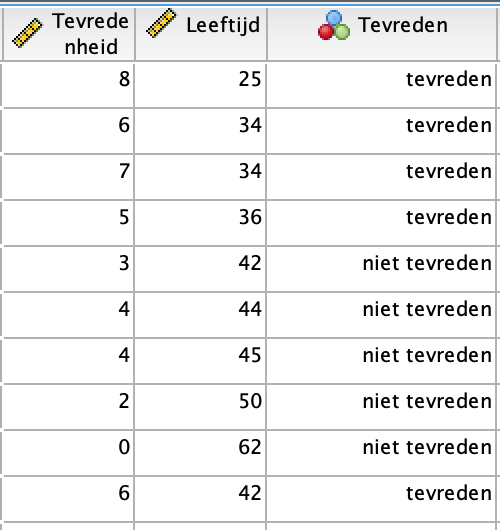
\includegraphics[width=0.5\linewidth]{img/ex_spss_log_1} \caption{Data voor tevredenheid}\label{fig:exspsslog1}
\end{figure}

Ga naar \texttt{analyze\ \textgreater{}\ regression\ \ \textgreater{}\ binary\ logistic} en vul daar volgende gegevens aan:

\begin{figure}
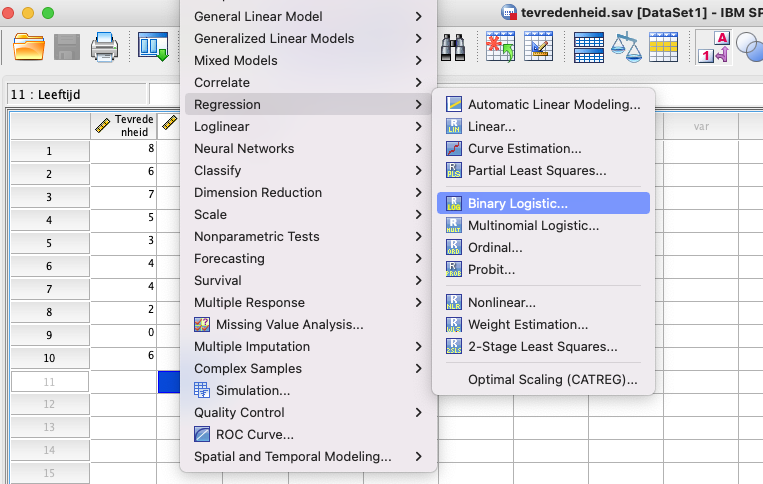
\includegraphics[width=1\linewidth]{img/ex_spss_log_2} \caption{Model invullen}\label{fig:exspsslog2}
\end{figure}

Let er op dat we tevredenheid onder dependent (afhankelijk) plaatsen en leeftijd onder het ``block''. Klik hierna op \texttt{Options...} en selecteer onder de statistieken ``CI for exp(B)'' and ``Hosmer-Lemeshowgoodness-of-fit''. Klik hierna op \texttt{Paste} en voer de Syntax uit.

\begin{figure}
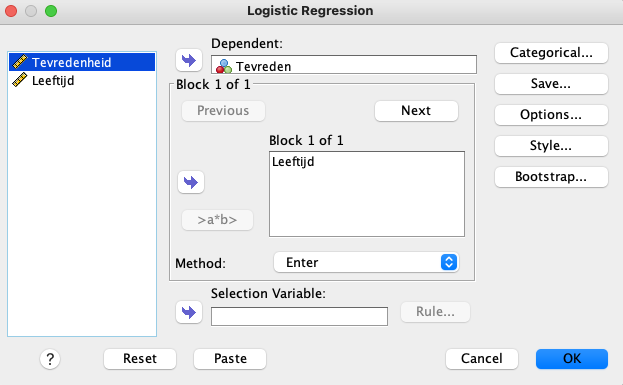
\includegraphics[width=1\linewidth]{img/ex_spss_log_3} \caption{Model invullen}\label{fig:exspsslog3}
\end{figure}

Wanneer je de input \texttt{paste} in de syntax en uit voert, zal je merken dat {SPSS} een intyerne codering uitvoert zoals aangegeven in figuur \ref{fig:exspsslog4}. De uitkomst \texttt{niet\ tevreden} van de variabele van de binaire variabele\texttt{tevreden} werd gehercodeerd naar 0, terwijl de uitkomst \texttt{tevreden} werd gehercodeerd naar 1.

\begin{figure}
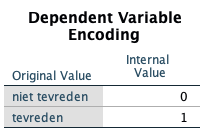
\includegraphics[width=0.4\linewidth]{img/ex_spss_log_4} \caption{Hercodering binnen SPSS}\label{fig:exspsslog4}
\end{figure}

\begin{exercise}
Kan je in de output het regressiemodel terugvinden?
\end{exercise}

\begin{exercise}
Is er een significant verband tussen de leeftijd en de score voor tevredenheid? Waaruit leid je dit af?
\end{exercise}

\begin{exercise}
Wat valt er op aan het model? Denk je dat het hier om een valide model gaat? Of zijn er eventuele problemen die we moeten aanpakken? Indien er problemen zijn, kan je dan opmerken waaraan deze problemen kunnen liggen?
\end{exercise}

\mainmatter

\hypertarget{multiregr}{%
\chapter{Meervoudige regressie}\label{multiregr}}

\hypertarget{inleiding-2}{%
\section*{Inleiding}\label{inleiding-2}}


Voorgaande hoofdstukken waren vooral gefocust op een regressievergelijking, waarbij de afhankelijke uitkomst (\(Y\)) wordt verklaard aan de hand van één onafhankelijke factor (\(X\)). Uiteraard weten we dat er in werkelijkheid vaak meer dan één factor gerelateerd zal zijn aan de uitkomst.

\textbf{Voorbeeld:} Wanneer we een idee willen hebben over het functioneren van een patiënt 3 jaar na het plaatsen van een totale heupprothese. Hiervoor kunnen we gebruik maken van een WOMAC score. Bij enkelvoudige regressie kunnen we focussen op het verband tussen deze WOMAC-score en bijvoorbeeld de leeftijd. Bij meervoudige regressie willen we echter ook rekening houden met andere factoren, zoals het geslacht, maar ook misschien het BMI of het al dan niet ervaren van comorbiditeiten. We bouwen hierbij nog steeds één model, dat al deze factoren omvat.

Meervoudige regressie (zowel lineair als binair) wordt dus vooral gebruikt in de volgende context: * Meenemen van covariaten * Nagaan van interacties * \ldots{}

Een \textbf{nadeel} van meervoudige regressie is dat het meenemen van meer variabelen vaak gepaard gaat met de nood aan een grotere steekproef.

\hypertarget{visualizatie}{%
\section*{Visualizatie}\label{visualizatie}}


Een manier om een regressiemodel te visualiseren is de Directed acyclic graph (DAG), hierbij worden factoren aan elkaar gerelateerd door pijlen. Een voorbeeld hiervan is weergegeven in figuur \ref{fig:dag1}. Hierbij merken we op dat er een pijl wordt getrokken van de exposure (blootstelling) naar de outcome (uitkomst). De DAG wil hiermee visualiseren dat er een theoretische invloed is van een bepaalde blootstelling (bv. de leeftijd) op een bepaalde uitkomst (bv. spierkracht). Een belangrijke \textbf{opmerkingen} hierbij is dat de pijl een theoretisch concept is, waarbij er veronderstelt wordt dat er een invloed is van één factor op de andere. Uiteraard weten we dat zo een oorzaak-gevolg relatie alleen duidelijk kan worden in een gerandomiseerde studie. Bij observationele studie zonder randomisatie, stelt de pijl eerder een `associatie' voor.

\begin{figure}
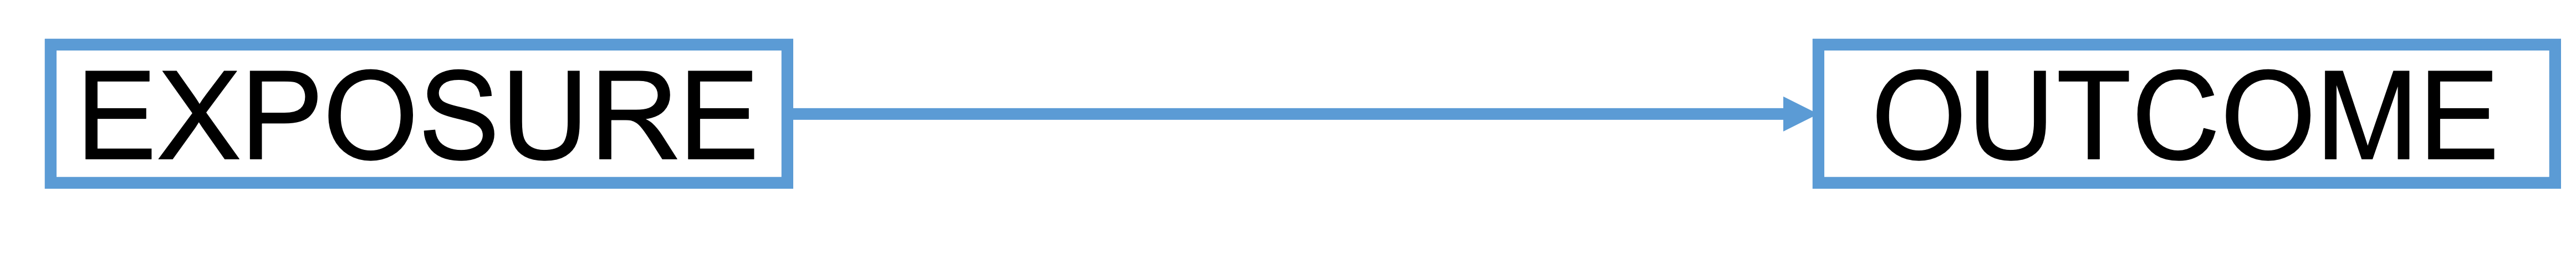
\includegraphics[width=0.75\linewidth]{img/dag1} \caption{Voorbeeld van DAG}\label{fig:dag1}
\end{figure}

Wanneer we het principe van de DAG gaan toepassen op basis van de studieresultaten die werden weergegeven in figuur \ref{fig:dag3}, krijgen we een DAG zoals weergegeven in figuur \ref{fig:dag2}. Het is belangrijk om te vermelden dat we ons ook bij een meervoudig regressiemodel, focussen op één van de opgenomen factoren (in dit geval de leeftijd). Het meervoudige regressiemodel is weergegeven in de rechterkolom van figuur \ref{fig:dag3}. Dit is aangegeven in de titel van de tabel dor het woord \textbf{multivariate}. We merken dat er drie factoren werden opgenomen, namelijk leeftijd, het al dan niet hebben van lage rugpijn en kwaliteit van leven (SF-36).

\begin{figure}
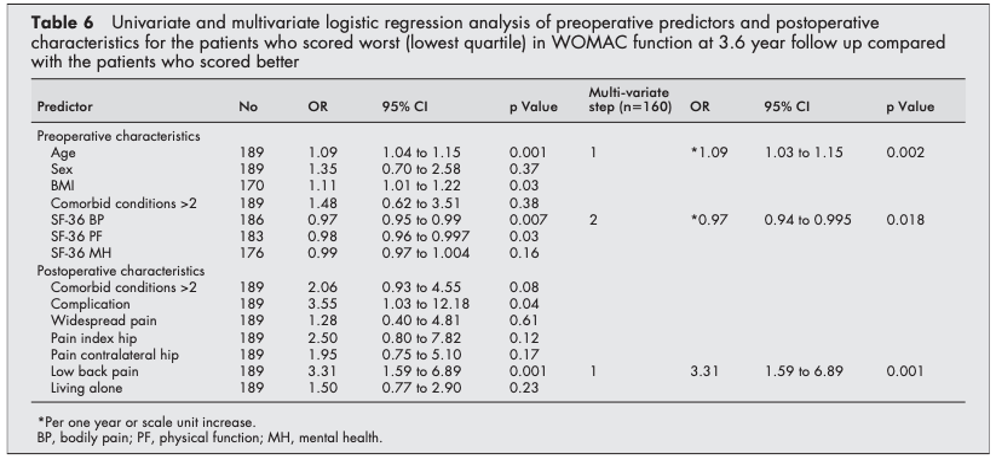
\includegraphics[width=0.75\linewidth]{img/dag3} \caption{Studie naar WOMAC}\label{fig:dag3}
\end{figure}

Binnen de DAG zoals weergegeven in figuur \ref{fig:dag2}, werd er gefocust op de relatie tussen { de leeftijd en WOMAC score }. Verder werd deze relatie binnen het meervoudige regressiemodel gecorrigeerd voor { het hebben van lage rugpijn } en { kwaliteit van leven }. De relatie tussen leeftijd en WOMAC wordt m.a.w. gecorrigeerd voor andere covariaten (soms ook benoemd als confounding of vervuilende variabelen). We kunnen deze oefening herhalen voor elk van de relaties binnen het meervoudige regressiemodel.

\begin{figure}
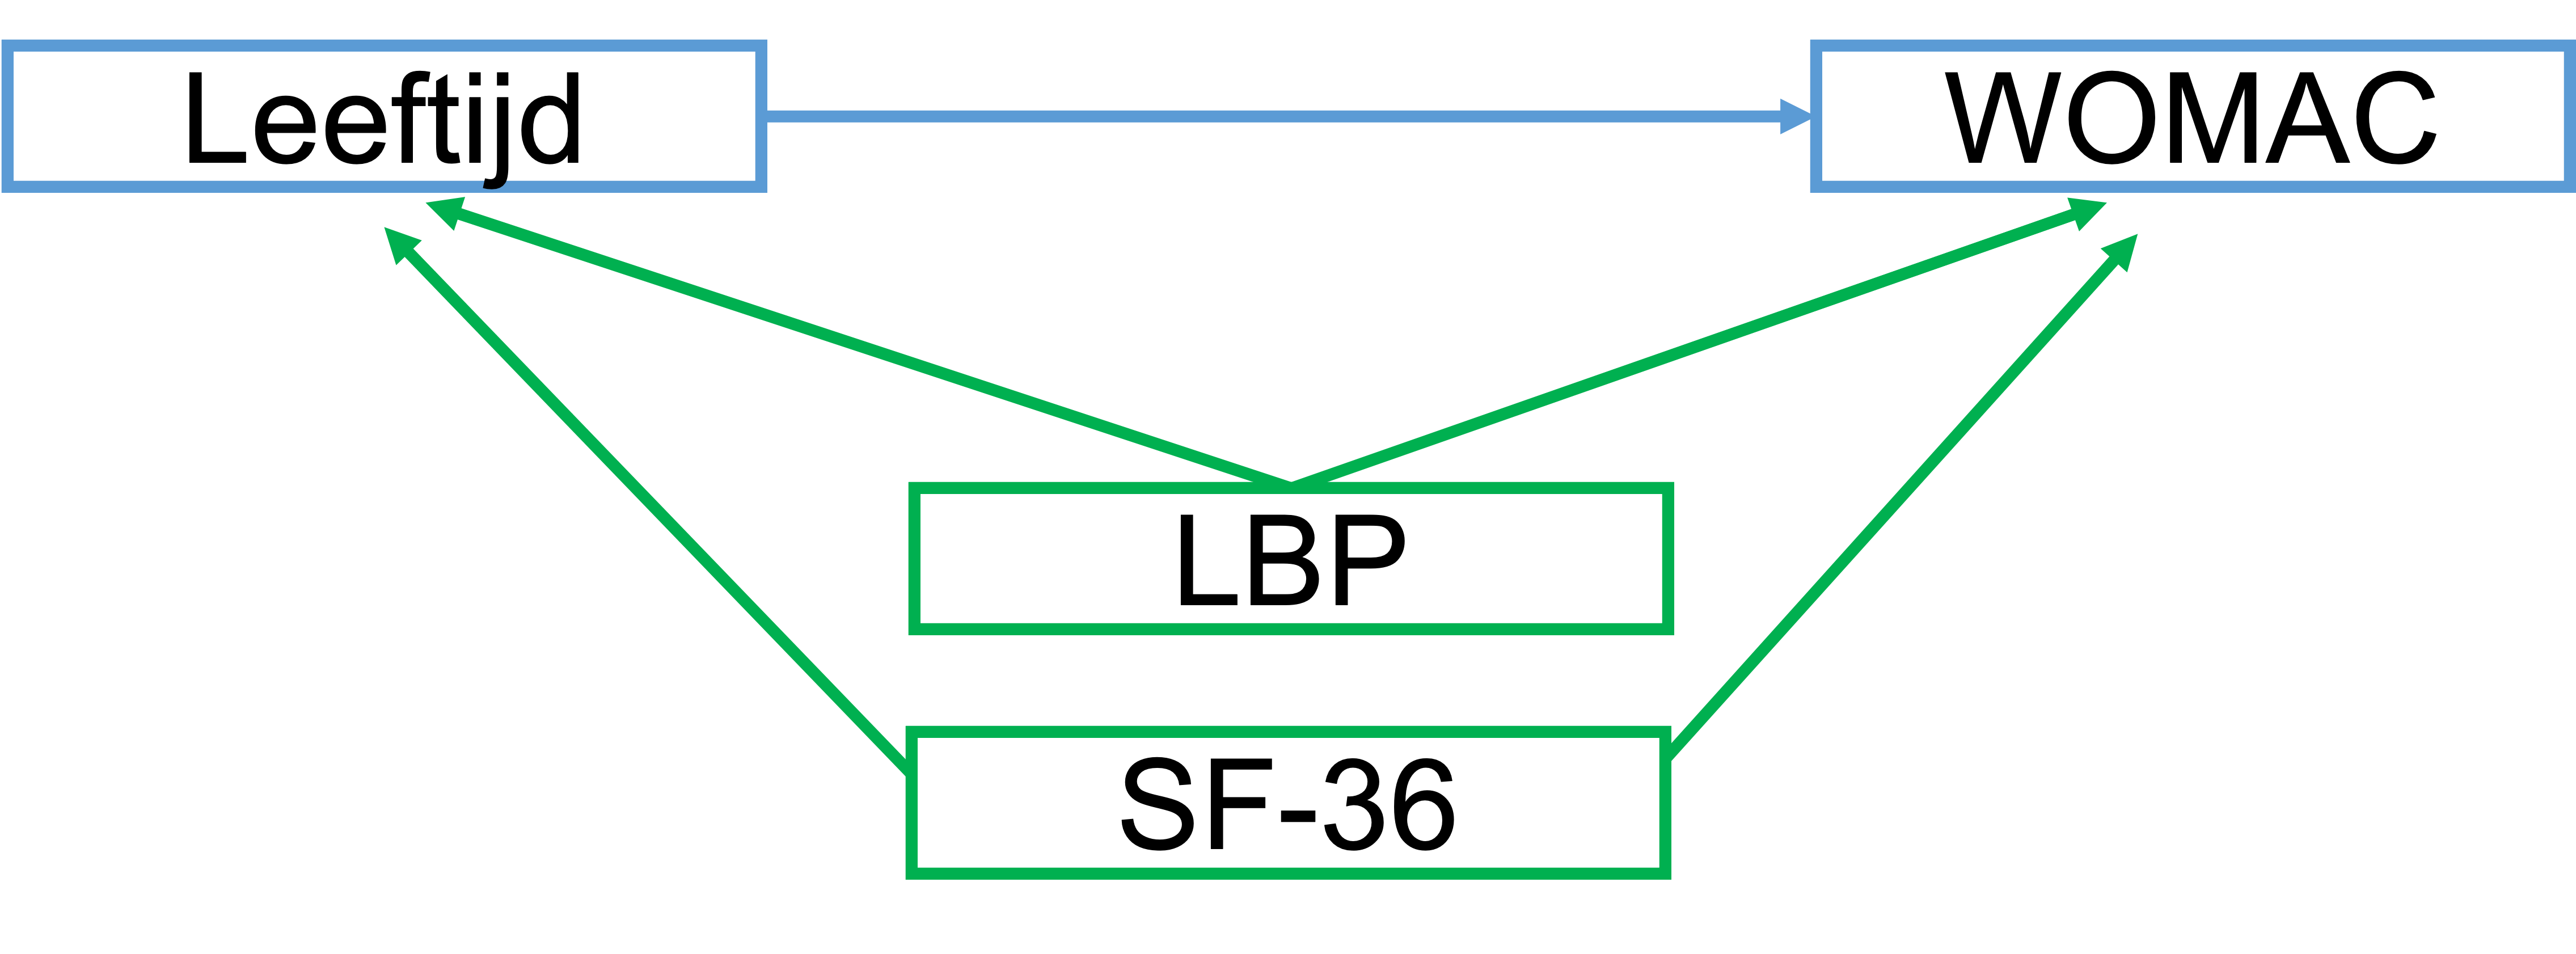
\includegraphics[width=0.75\linewidth]{img/dag2} \caption{DAG voor WOMAC-studie}\label{fig:dag2}
\end{figure}

\hypertarget{terminologie}{%
\section*{Terminologie}\label{terminologie}}


Vooraleer gebruik te maken van zo'n DAGs is het belangrijk om op de hoogte te zijn van de terminologie. In de eerste plaats is het belangrijk een onderscheid te maken tussen een \textbf{collider} en een \textbf{confounder}. Een \textbf{collider} ontstaan wanneer in werkelijkheid 2 factoren de onderliggende oorzaak zijn van een andere factor zoals weergegeven in figuur \ref{fig:dag4}. Wanneer we in ons model zouden corrigeren voor een \textbf{collider}, dan ontstaat er net bias.

\begin{figure}
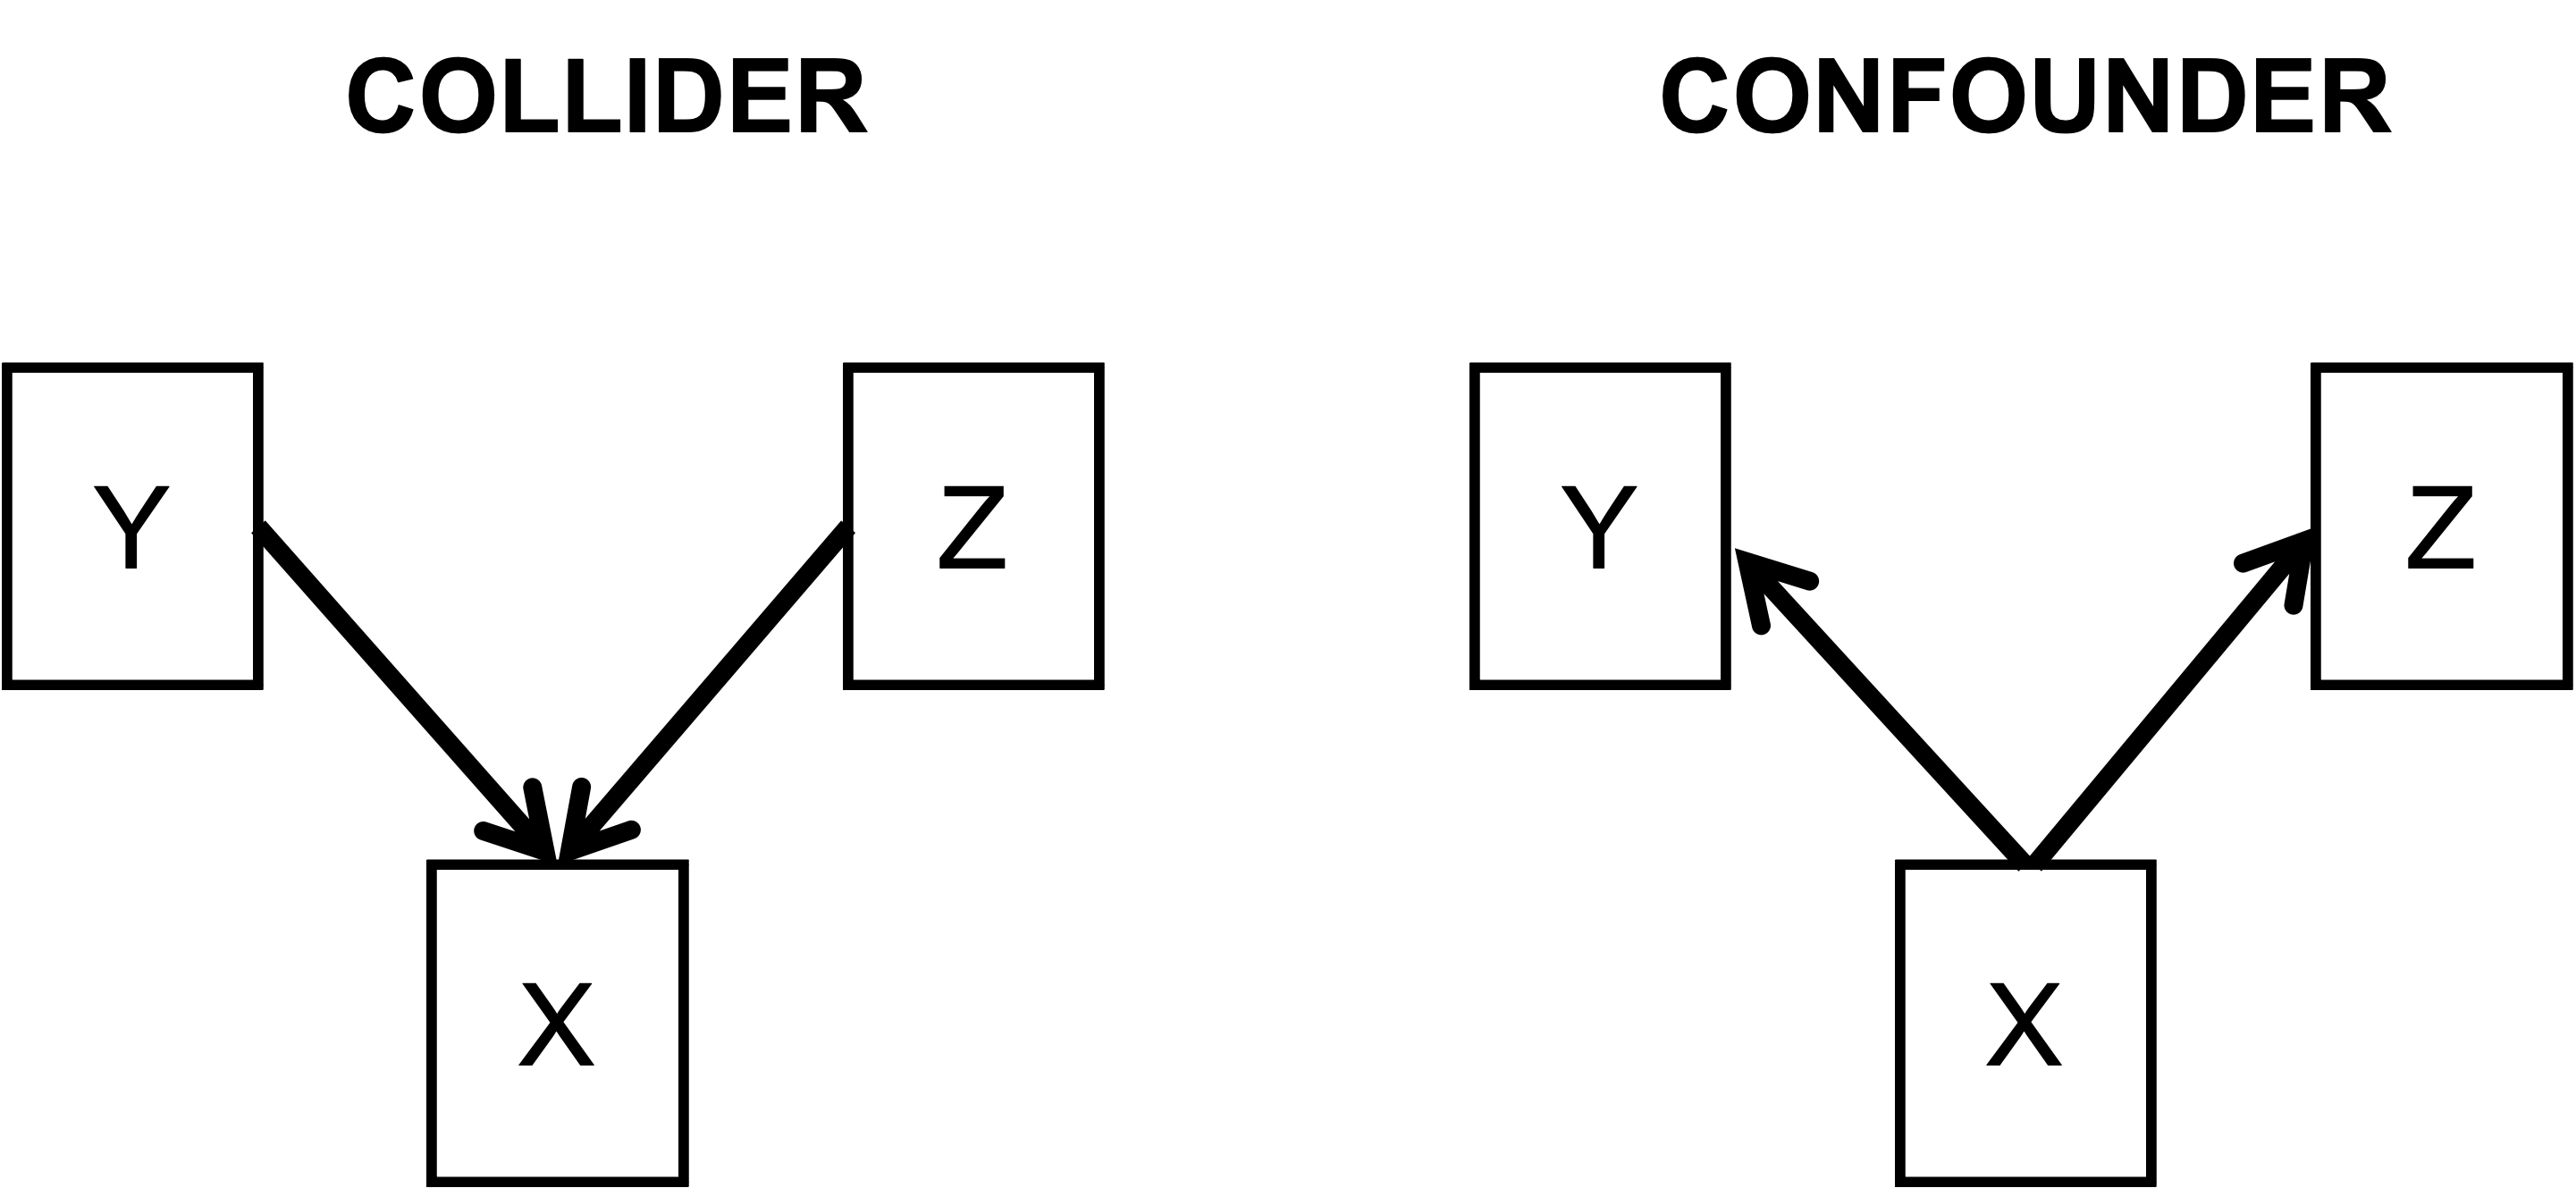
\includegraphics[width=0.75\linewidth]{img/dag4} \caption{Voorbeeld van DAG}\label{fig:dag4}
\end{figure}

Een concreet voorbeeld van zo'n \textbf{collider} bias is de obesitas paradox. In deze paradox lijkt het alsof obesitas zorgt voor een verlaagde mortaliteit bij patiënten met een cardiovasculaire aandoening. Wanneer we dus obesitas samen met een cardiovasculaire aandoening in één model, ontstaat er collider bias. Het is namelijk zo dat binnen de groep van patiënten met zo'n aandoening, dat deze patiënten - wanneer ze opgenomen worden in het ziekenhuis - langer lijken te overleven. Wanneer we echter kijken binnen de volledige populatie, is het duidelijk dat obesitas leidt tot een verhoogde sterfte. Mensen met obesitas hebben misschien wel meer reserves, waardoor hun overlevingstijd langer wordt wanneer we enkel kijken naar de mensen die leiden aan andere aandoeningen. \textbf{Belangrijk} hierbij is te weten dat het opnemen van covariaten dus niet steeds leidt tot het corrigeren van een relatie.

\begin{figure}
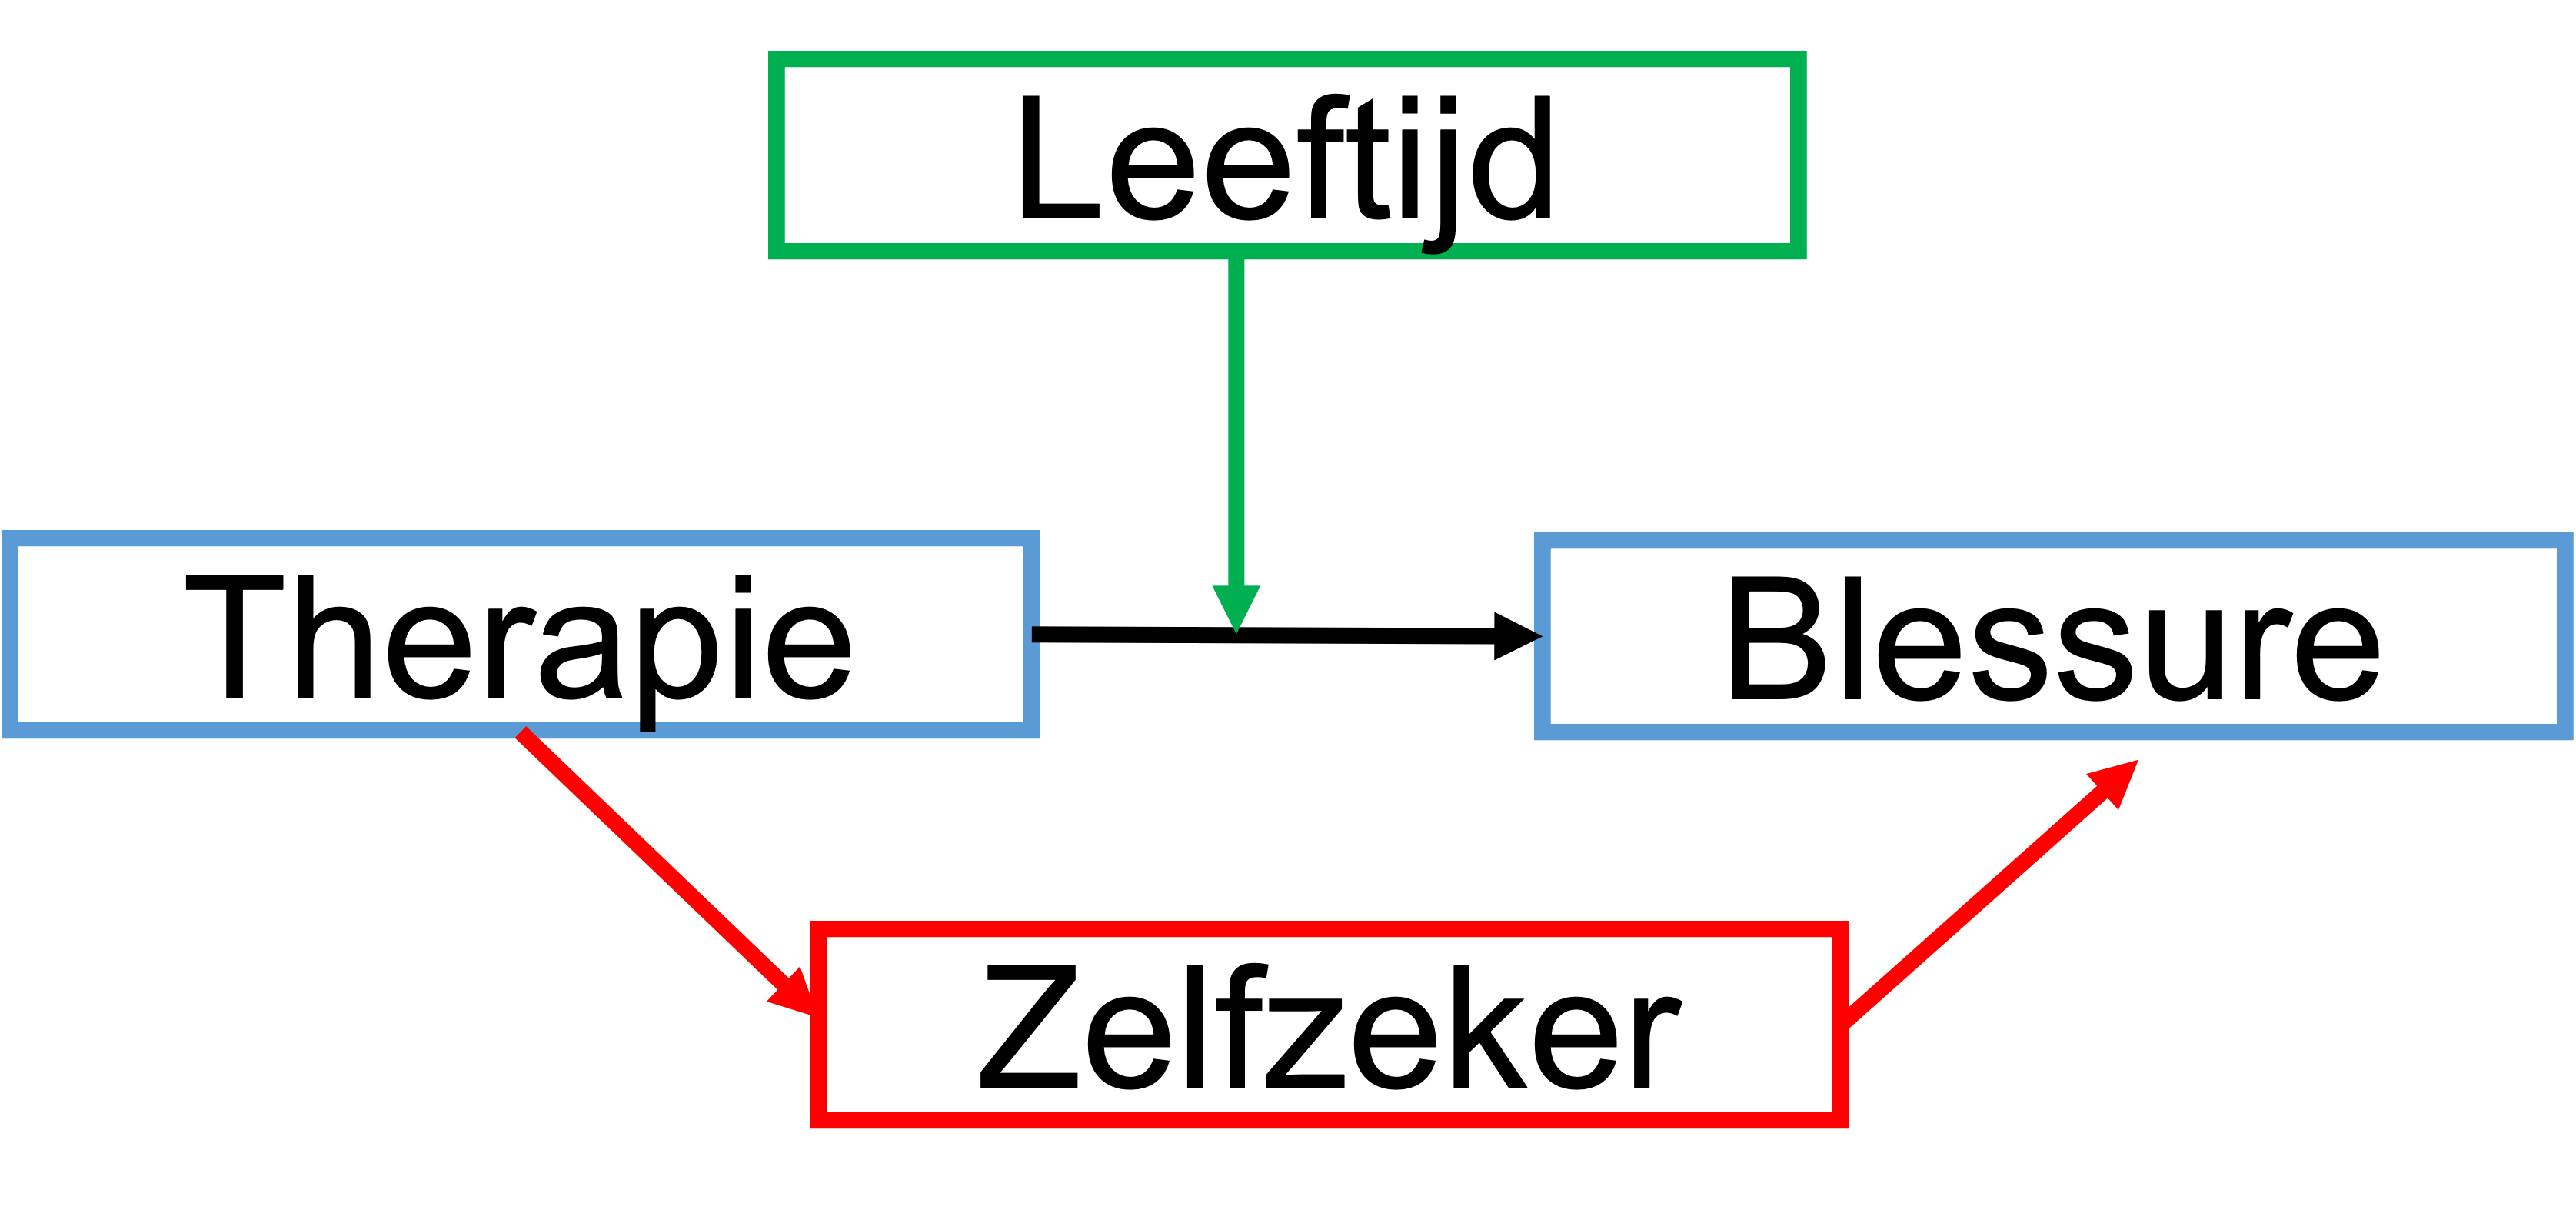
\includegraphics[width=0.75\linewidth]{img/dag5} \caption{Terminologie van een DAG}\label{fig:dag5}
\end{figure}

Binnen de DAG die weergegeven is in figuur @ref(fig: dag5) worden de verschillende relatie weergegeven:

\begin{itemize}
\tightlist
\item
  {Directe effect}: deze geeft het directe effect weer van het geven van een therapie op het oplopen van blessures.
\item
  {Moderatie}: een modererende factor is een factor die een invloed heeft op de relatie tussen twee factoren.
\item
  {Mediatie}: een mediërende factor is een factor die onrechtstreeks een invloed weergeeft tussen twee factoren. Deze worden ook indirecte effecten genoemd.
\end{itemize}

In het voorbeeld, wordt het directe effect weergegeven door een direct effect van de therapie op het al dan niet oplopen van blessures. De mediator in dit voorbeeld is zelfzeker zijn. De therapie kan immers ervoor zorgen dat de sporter zijn zelfzekerheid veranderd (toeneemt of afneemt) wat ook een effect kan hebben op het al dan niet oplopen van blessures. Tot slot is er de leeftijd als moderator. Het is immers zo dat mensen met een oudere leeftijd misschien minder effect hebben van de therapie in vergelijking met jongeren. De leeftijd heeft dus een invloed op het effect van de therapie. Deze modererende effecten worden in een model vaak geschat op basis van een interactie-effect.

\hypertarget{toepassingen-dag}{%
\section*{Toepassingen DAG}\label{toepassingen-dag}}


In een gerandomiseerde studie vonden de onderzoekers een positief effect van kinesitherapie op kwaliteit van leven bij patiënten na een knie-prothese. Binnen deze studie werd er gevonden dat de effectiviteit veel hoger lag bij jongere patiënten ten opzichte van oudere patiënten.

Hoe kunnen we de rol van leeftijd definiëren? \emph{Leeftijd} is in dit geval een moderator.

In een gerandomiseerde studie vonden de onderzoekers een positief effect van kinesitherapie op kwaliteit van leven bij patiënten na een knie-prothese. Binnen deze studie werd er gevonden dat de effectiviteit veel hoger lag bij jongere patiënten ten opzichte van oudere patiënten.

Moeten we corrigeren voor geslacht in deze studie wanneer we weten dat geslacht een mogelijke confounder is? \emph{Eigenlijk niet}, aangezien de studie gerandomiseerd is. Randomisatie wil zeggen dat de therapie enkel gebaseerd is op toeval en er geen factoren zijn die van invloed kunnen zijn op de therapie.

In een niet-gerandomiserde studie vonden de onderzoekers een positief effect van kinesitherapie op kwaliteit van leven bij patiënten na een knie-prothese. Binnen deze studie werd er gevonden dat de effectiviteit veel hoger lag bij jongere patiënten ten opzichte van oudere patiënten. Belangrijke confounders zijn geslacht en mate kan kinesiofobie.

Hoe zou een DAG eruit zien? \emph{Zie figuur \ref{fig:dag6}}

\begin{figure}
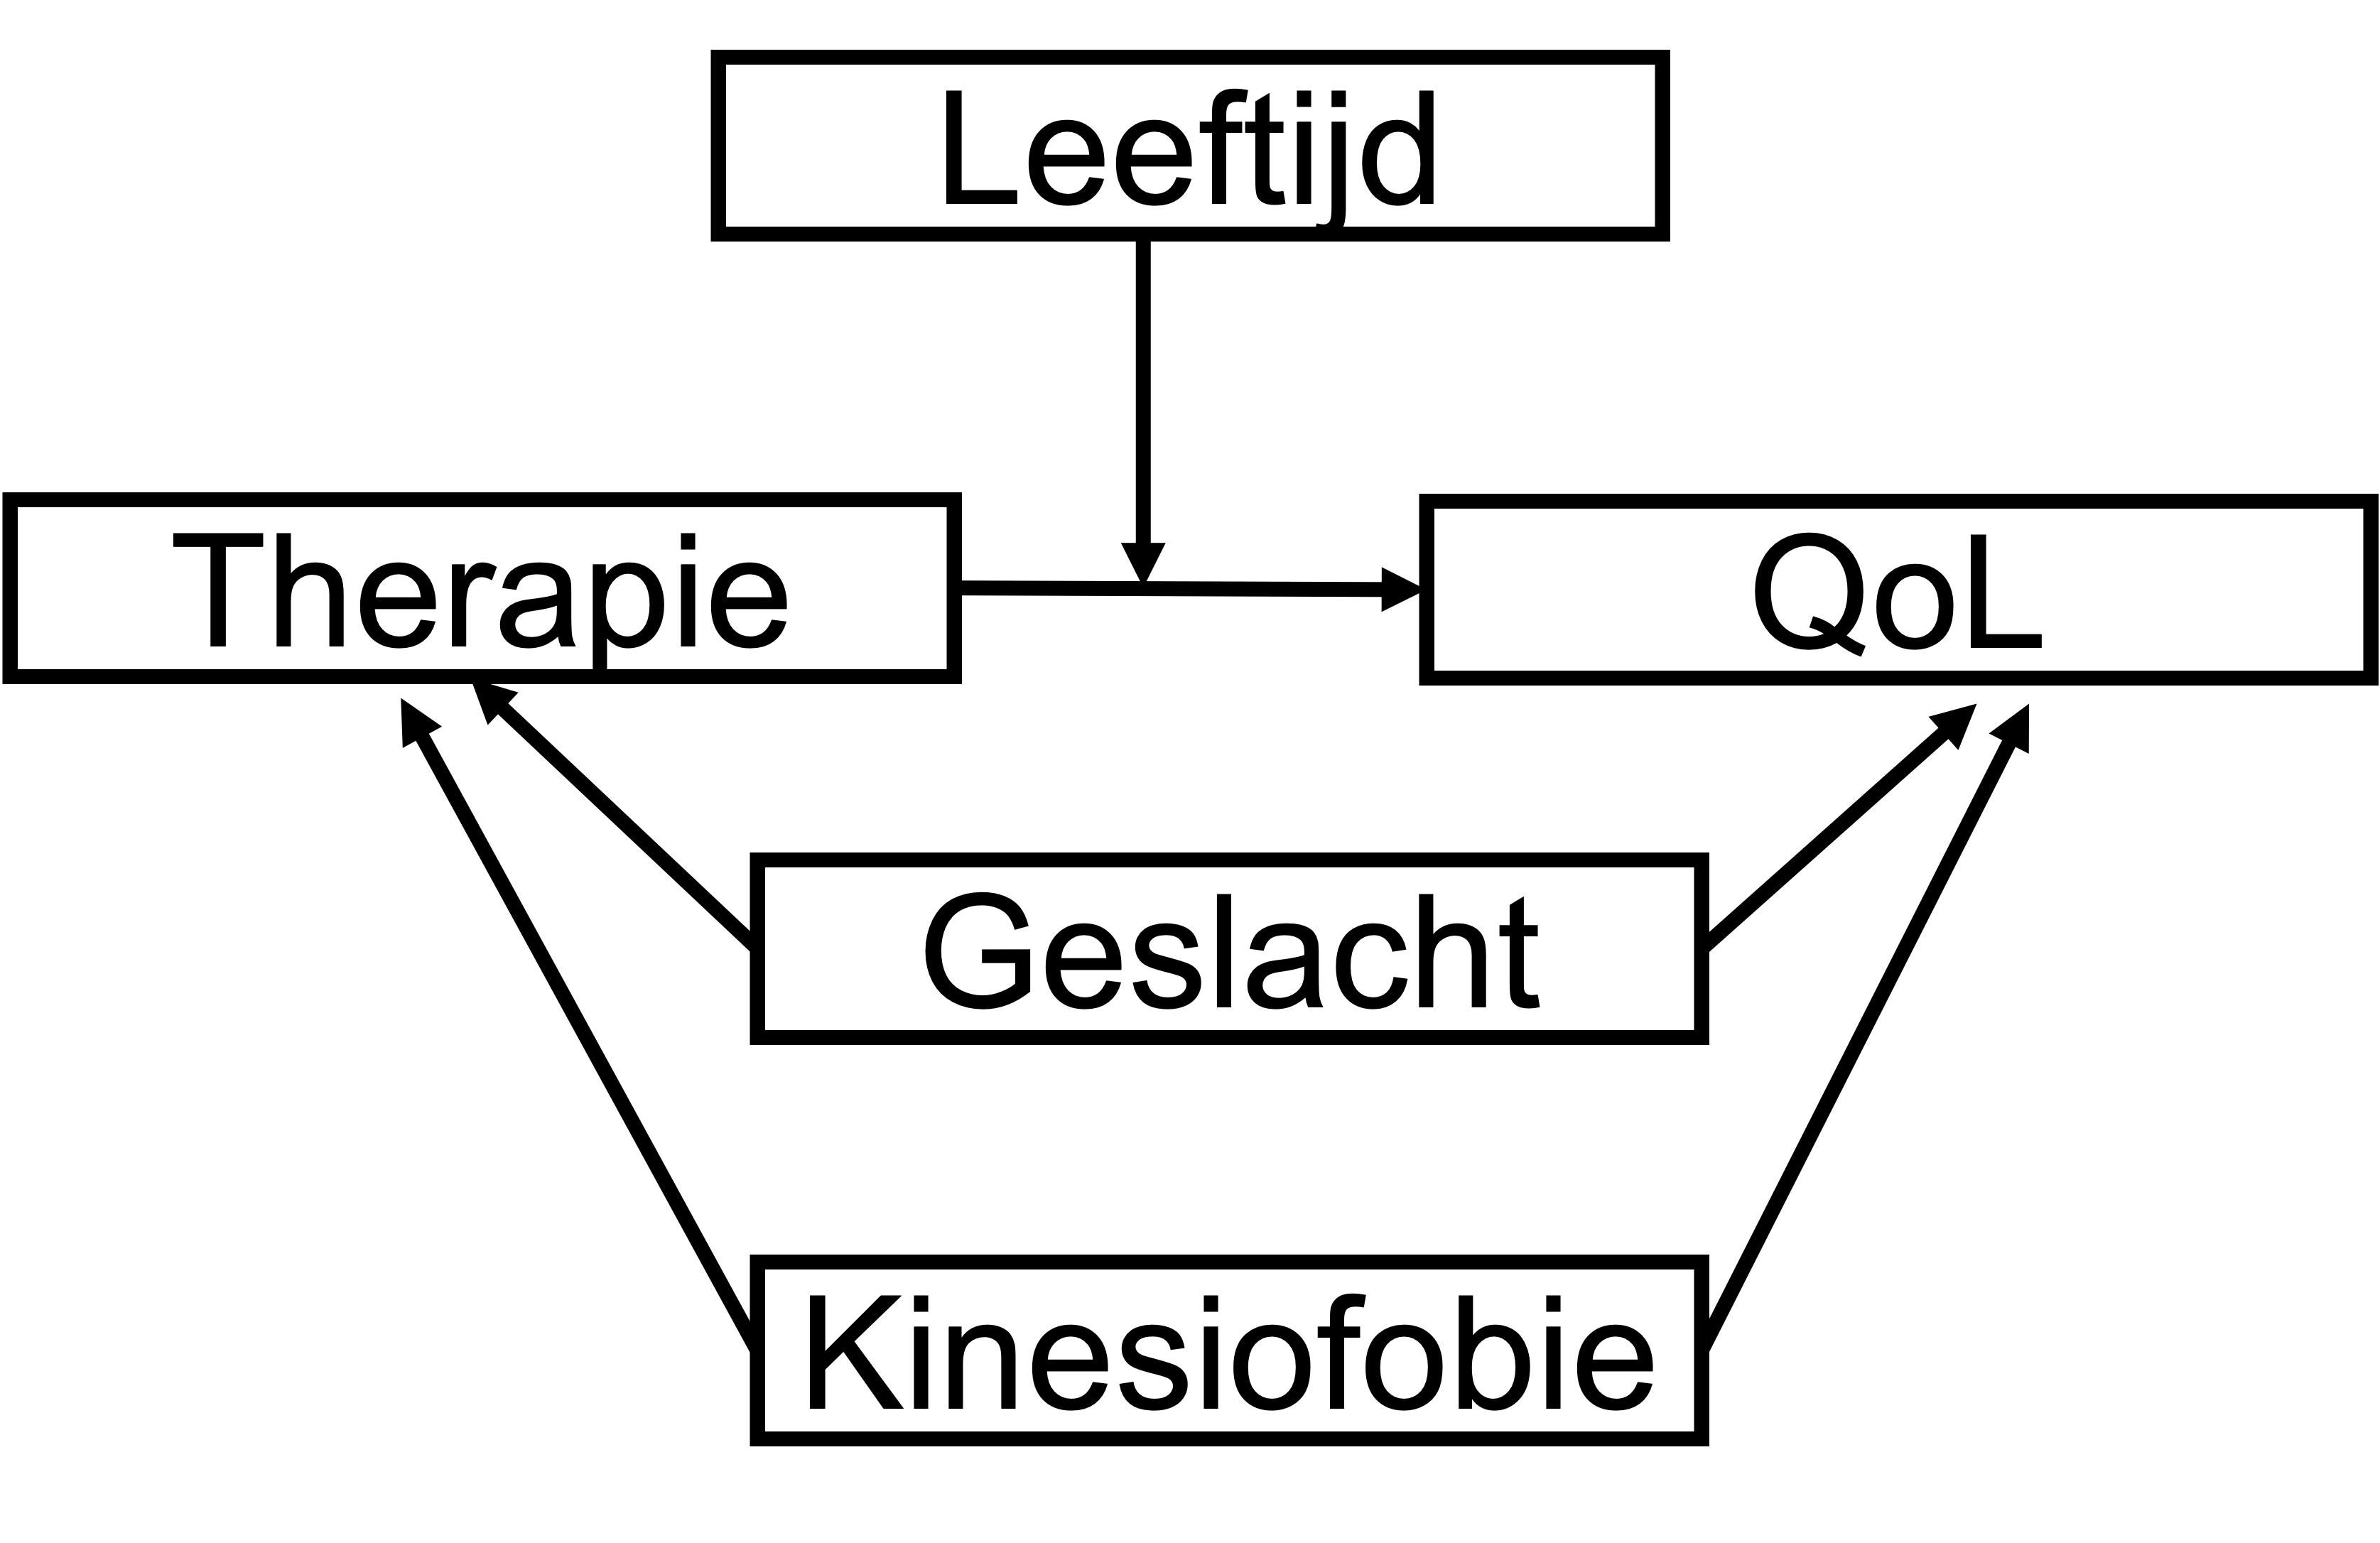
\includegraphics[width=0.75\linewidth]{img/dag6} \caption{DAG}\label{fig:dag6}
\end{figure}

\hypertarget{meervoudige-regressie}{%
\section*{Meervoudige regressie}\label{meervoudige-regressie}}


Een meervoudig lineair regressiemodel wordt weergegeven aan de hand van \(Y = \beta_0 + \beta_1X_1 + \beta_2X_2+...+\epsilon\). Binnen deze regressievergelijking kunnen we confounder opnemen en kunnen we ook interactie-effecten (moderatie) opnemen, maar geen mediatie.

\hypertarget{confounder}{%
\subsection*{Confounder}\label{confounder}}


Een voorbeeld van de interpretatie van een regressiemodel wanneer we confounder opnemen is als volgt:

Meervoudige regressie: opnemen van meerdere factoren \textgreater\textgreater{} correctie van het effect voor de andere factoren.

\(Tevredenheid = \beta_0 + \beta_1 \times leeftijd + \beta_2 \times geslacht(man)\)

\begin{itemize}
\tightlist
\item
  \(\beta_1\) = inschatting van het effect van leeftijd op tevredenheid gecorrigeerd voor geslacht.
\item
  \(\beta_2\) = inschatting van het effect van geslacht op tevredenheid gecorrigeerd voor leeftijd.
\end{itemize}

\hypertarget{moderatie}{%
\subsection*{Moderatie}\label{moderatie}}


Bij een moderatie-analyse wordt er gebruik gemaakt van interacties. Een interactie wordt als volgt weergegeven in een regressievergelijking:

\(Y = \beta_0 + \beta_1 \times X_1 + \beta_2 \times X_2 + \beta_3 \times X_1 \times X_2 + \epsilon\)

\(\beta_3\) geeft in deze formule de interactie weer tussen \(X_1\) en \(X_2\). De interpretatie van \(\beta_3\) is echter moeilijk op basis van bovenstaande formule. WAnneer we deze formule herschrijven als

\(Y = \beta_0 + \beta_2 \times X_2 + (\beta_1 + \beta_3 \times X_1) \times X_2 + \epsilon\),

kunnen we heft effect van deze \(\beta_3\) beter evalueren. De associatie tussen \(Y\) en \(X_2\) wordt nu weergegeven door \((\beta_1 + \beta_3 \times X_1)\), waarbij de associatie:

\begin{itemize}
\tightlist
\item
  \(\beta_1 + \beta_3\) is wanneer \(X_1 = 1\)
\item
  \(\beta_1\) is wanneer \(X_1 = 0\)
\end{itemize}

Stel dat \(Y = tevredenheid\), \(X_1 = leeftijd\) en \(X_2 = geslacht\). Wanneer er bij mannen een toename zou zijn in tevredenheid bij een stijgende leeftijd en bij vrouwen een afname in tevredenheid bij een stijgende leeftijd, dan is er een interactie-effect, waarbij \(\beta_3\) significant zal zijn.

Een visuele weergave van een interactie-effect is terug te vinden in figuur \ref{fig:int1}. Zwart geeft de associatie weer voor vrouwen, terwijl lichtgrijs de assocaitie weergeeft voor mannen.

\begin{figure}
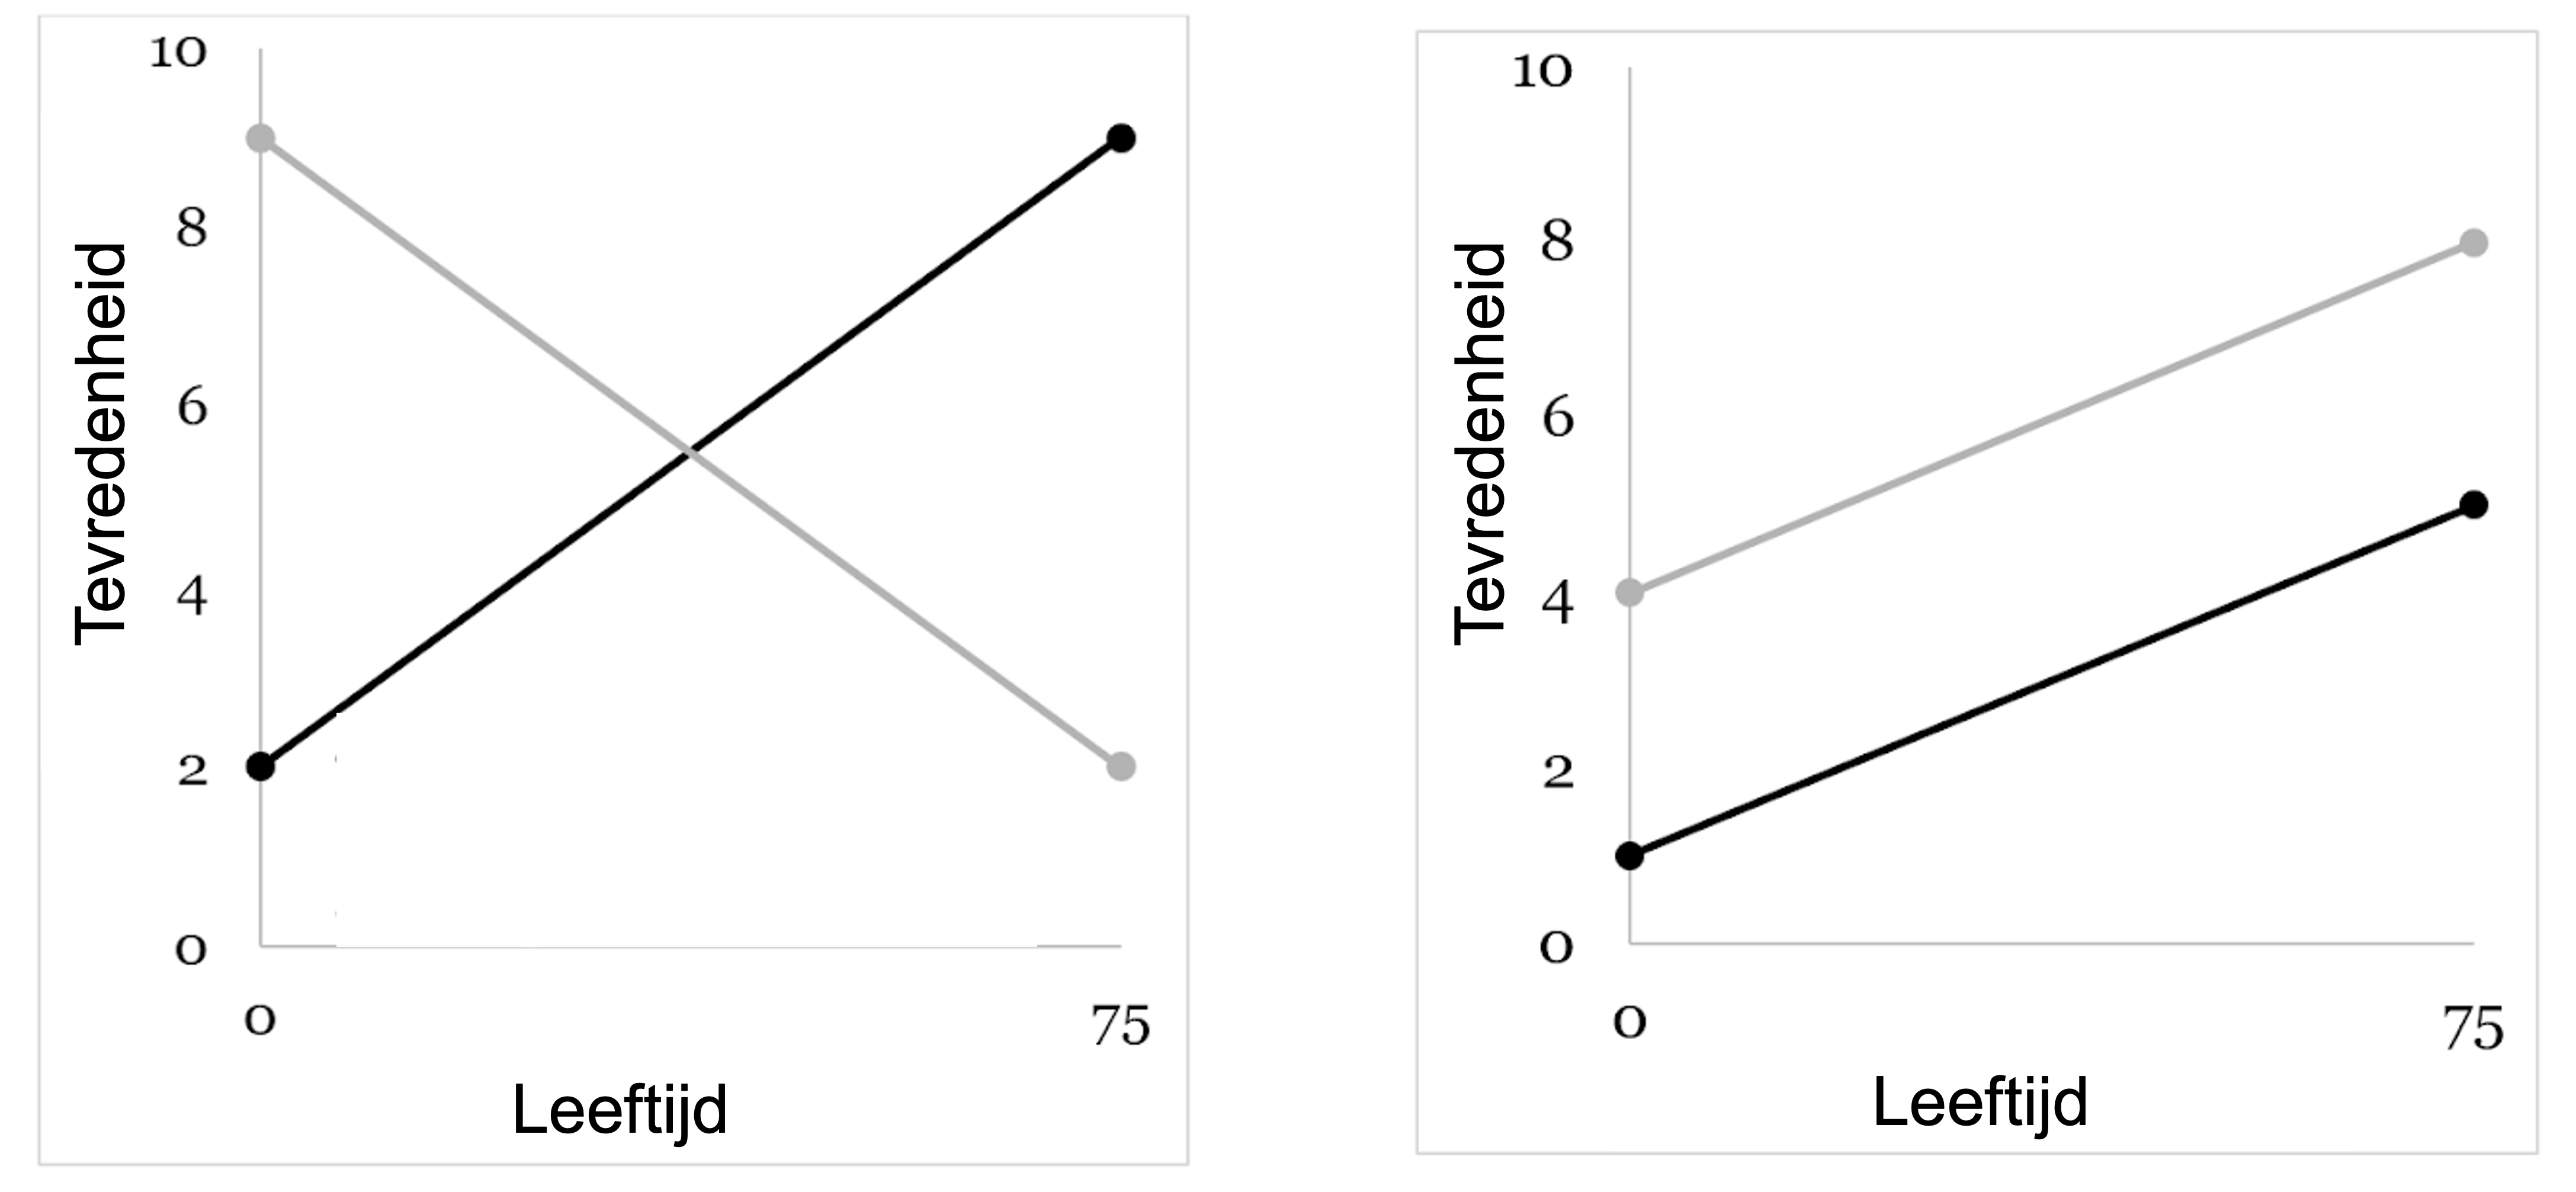
\includegraphics[width=0.75\linewidth]{img/interactie1} \caption{DAG}\label{fig:int1}
\end{figure}

We kunnen intreactie of moderatie-effecten gebruiken voor alle combinaties van variabelen:

\begin{itemize}
\tightlist
\item
  categrosch x categorisch
\item
  categorisch x continu
\item
  continu x continu
\end{itemize}

\hypertarget{selectie-van-het-meest-passende-regressiemodel}{%
\section*{Selectie van het meest passende regressiemodel}\label{selectie-van-het-meest-passende-regressiemodel}}


Lineaire regressie: * \(R^2\) (determinatiecoëfficiënt) moet zo hoog mogelijk zijn * Geweten confounders * Significantie van de variabelen in het model

Logistische regressie: * Naglekerke's \(R^2\) (determinatiecoëfficiënt) moet zo hoog mogelijk zijn * Geweten confounders * Significantie van de variabelen in het model * Zo hoog mogelijk: Acc, Se of Sp.

\mainmatter

\hypertarget{exam}{%
\chapter{Voorbeeldexamen}\label{exam}}

Om dit voorbeeld examen te kunnen maken dien je te beschikken over een SPSS (.sav) dataset. Om deze dataset te downloaden kan je op volgende knop duwen:

\hypertarget{inleiding-3}{%
\subsection*{Inleiding}\label{inleiding-3}}


Dit voorbeeldexamen geeft een reële indruk van de verwachtingen op het examen met betrekking tot jullie kennis en vaardigheden binnen SPSS. Aan de hand van deze vragen, zouden jullie in staat moeten zijn om alle vragen binnen dit voorbeeld examen op te lossen. Zoals jullie zien, zal het examen bestaan uit drie delen: (1) een praktisch deel waar jullie aan de slag kunnen gaan met SPSS en (2) een praktisch deel met fragmenten uit een artikel dat jullie dienen te interpreteren en (3) een laatste deel met enkele korte theoretische vragen over de geziene stof. Als alles goed gaat, zouden jullie in staat moeten zijn om dit voorbeeld examen binnen het uur op te lossen.

\hypertarget{deel-i}{%
\subsection*{DEEL I}\label{deel-i}}


Neem de dataset SPSS\_DATA\_REVAKI.sav (die je hierboven kan downloaden) en open deze in SPSS. Probeer hierna alle vragen op een correcte manier te beantwoorden. Alle info over deze dataset vinden jullie binnen het variable-frame van SPSS.

Maak een lineair regressiemodel waarbij de afhankelijke variabelen de CRP-waarden in het bloed is en de onafhankelijke variabelen diabetes (REF = geen diabetes), leeftijd (jaren) en geslacht (REF = man). Beantwoordt hierna volgende vragen. Voor alle duidelijkheid, de referentiecategorie (REF) is de categorie die geassocieerd moet worden met waarde 0.

\begin{exercise}
Selecteer de meest gepaste R² van het model en schrijf deze neer.
\end{exercise}

\begin{exercise}
Hoeveel observaties zitten er in het model?
\end{exercise}

\begin{exercise}
Kan je tot twee cijfers na de komma weergeven wat de associatie is tussen CRP en leeftijd (per 10 jaar)?
\end{exercise}

\begin{exercise}
Noteer hieronder de variabelen die significant zijn (van sterkste associatie naar zwakste associatie in absolute eenheden).
\end{exercise}

Maak een logistisch regressiemodel waarbij de afhankelijke variabele de status van de patiënt is (waarbij we als uitkomst kijken naar tranferred patiënten). Als onafhankelijke variabelen kunnen jullie gebruik maken van leeftijd, geslacht (REF = vrouw), obesitas, hoge bloed druk en cardiovasculaire aandoeningen (hierbij is bij alle comorbiditeiten ``niet aanwezig'' de REF). Beantwoord hierna volgende vragen.

\begin{exercise}
Wat is de OR voor cardiovasculair risico?
\end{exercise}

\begin{exercise}
Hoeveel \% is extra correct geclassificeerd als we het model met variabelen beschouwen t.o.v. het model zonder variabelen?
\end{exercise}

\begin{exercise}
Wat is de p-waarde voor het model?
\end{exercise}

\begin{exercise}
Wat is het 95\% betrouwbaarheidsinterval rond de OR voor geslacht?
\end{exercise}

\hypertarget{deel-ii}{%
\subsection*{DEEL II}\label{deel-ii}}


Bekijk aandachtig de knipsel uit het artikel Bodin, J., Ha, C., Le Manac'h, A. P., Sérazin, C., Descatha, A., Leclerc, A., \ldots{} \& Roquelaure, Y. (2012). Risk factors for incidence of rotator cuff syndrome in a large working population. Scandinavian journal of work, environment \& health, 436-446. Beantwoordt op basis van deze knipsels de vragen zo correct mogelijk. Er is steeds maar één juist antwoord.

\begin{figure}
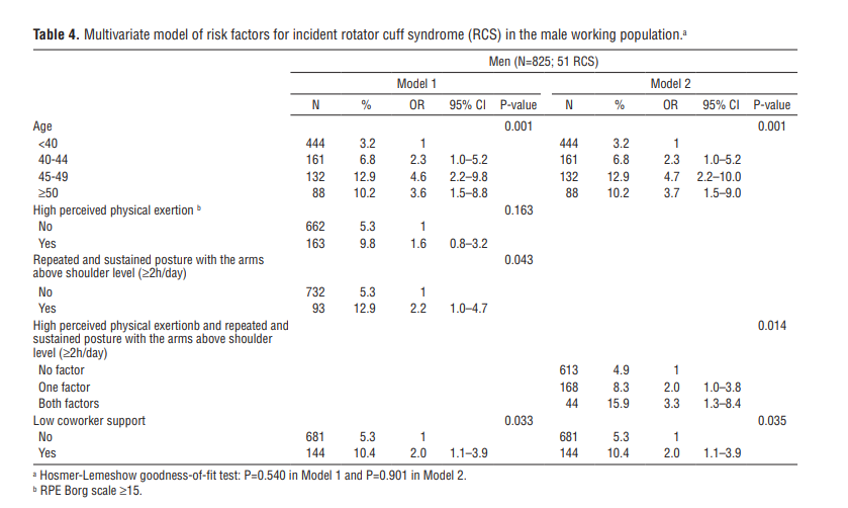
\includegraphics[width=0.9\linewidth]{img/exam_1} \caption{Bodin et al. (2012).}\label{fig:exam1}
\end{figure}

\begin{exercise}
Op basis van bovenstaande tabel zien we (onderaan) dat de Hosmer-Lemeshow test niet significant is. Wat kunnen we hieruit afleiden?

\emph{De model-fit is adequaat en zowel model 1 als model 2 zijn voldoende representatief. }De model-fit is inadequaat en de data en het model vertonen sterke discrepanties. \emph{De residuen zijn normaal verdeeld en alle voorwaarden van het model zijn voldaan. }De residuen zijn niet normaal verdeeld en niet alle voorwaarden van het model zijn voldaan.
\end{exercise}

\begin{exercise}
Multivariate model in de titel wil zeggen dat\ldots{}

\emph{Er rekening werd gehouden met andere mogelijke verstorende (confouding) variabelen. }De OR apart zijn berekend voor elk model en er dus mogelijks confounding kan zijn van de resultaten. \emph{Er rekening werd gehouden met meerdere afhankelijke variabelen in het model. }Geen van bovenstaande.
\end{exercise}

\begin{exercise}
Waarom is bij de leeftijdscategorie van \textless40 een OR van 1 weergegeven en geen 95\% CI berekend?

\emph{Deze categorie is de referentiecategorie waarmee we de andere categorieën dienen te vergelijken. }Dit wil zeggen dat de categorie \textless{} 40 jaar niet significant geassocieerd is met verhoogd of verlaagd risico. \emph{In deze categorie zaten er onvoldoende observaties om een uitspraak te kunnen doen. }Geen van bovenstaande.
\end{exercise}

\begin{exercise}
In bovenstaand model 2 is er voor de factor ``High perceived physical exertionb and repeated and sustained posture with the arms above shoulder level (more or equal then 2h/day)''.

\emph{Een significant verhoogd risico wanneer ``both factors'' aanwezig zijn t.o.v. ``one factor''. }Zijn de odds voor rotator cuff syndrome (RCS) 3.3 keer hoger in de groep waarbij ``both factors'' positief zijn t.o.v. ``no factor'' \emph{Er geen significant risico gevonden voor deze factor aangezien de p-waarde niet kleiner is dan 0.01. }Geen van bovenstaande.
\end{exercise}

\hypertarget{deel-iii}{%
\subsection*{DEEL III}\label{deel-iii}}


Probeer onderstaande theoretische vragen zo correct mogelijk te beantwoorden. Er is steeds maar één juist antwoord.

\begin{exercise}
Om een zo correct mogelijk model te bouwen met een lineaire regressie-analyse is het belangrijk dat:

\emph{Er een lineair verband bestaat tussen de onafhankelijke en afhankelijke uitkomstmaten. }De residuen niet normaal verdeeld zijn en een gelijke variantie hebben. \emph{De VIF-waarde kleiner is dan 1, zodat multicollineariteit zoveel mogelijk uitgesloten kan worden. }Geen van bovenstaande.
\end{exercise}

\begin{exercise}
Vul op een zo correct mogelijke manier volgende tabel aan. Geef aan welk cijfer je verwacht in de verschillende vakjes (tot 3 cijfers na de komma). Het gaan om een lineair regressiemodel met 4 ONafhankelijke variabelen.

\begin{figure}
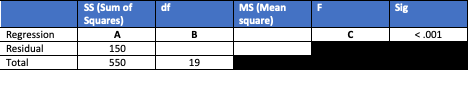
\includegraphics[width=0.9\linewidth]{img/exam_2} \caption{Invulexamen}\label{fig:exam2}
\end{figure}

Vul hierna de waarden in voor A, B en C.
\end{exercise}

\end{document}
